\documentclass[11pt]{article}

\usepackage{deauthor,times,graphicx}
\usepackage{color,colortbl}
% \usepackage[dvipsnames]{xcolor}
% \usepackage{hyperref}
\usepackage{amsmath}
\usepackage{amssymb}
\let\proof\relax
\let\endproof\relax
\usepackage{amsthm}
\usepackage{cleveref}
\usepackage{wrapfig}
\usepackage{url}
\usepackage{stmaryrd,amssymb}
\usepackage{listings}
\usepackage{algorithm}
% \usepackage[noend]{algorithmic}
\usepackage{fancybox}


%%%%%%%%%%%%%%%%%%%%%%%%%%%%%%%%%%%%%%%%
% Theorems, Definitions, Examples
%%%%%%%%%%%%%%%%%%%%%%%%%%%%%%%%%%%%%%%%
\newtheorem{theo}{Theorem}
\numberwithin{theo}{section}
\newtheorem{lem}[theo]{Lemma}
\newtheorem{propo}[theo]{Proposition}
\newtheorem{coll}[theo]{Corollary}
\newtheorem{exam}{Example}
\numberwithin{exam}{section}
\newtheorem{defi}{Definition}
\numberwithin{defi}{section}


%%%%%%%%%%%%%%%%%%%%%%%%%%%%%%%%%%%%%%%%%%%%%%%%%%%%%%%%%%%%%%%%%%%%%%%%%%%%%%%%
\usepackage{todonotes}
\newcommand{\BG}[1]{\todo[inline]{\textbf{Boris:} #1}}
\newcommand{\OK}[1]{\todo[inline]{\textbf{Oliver:} #1}}
\newcommand{\JF}[1]{\todo[inline]{\textbf{Juliana:} #1}}
\newcommand{\MB}[1]{\todo[inline]{\textbf{Mike:} #1}}

\newcommand{\jfedit}[1]{\textcolor{red} {#1}}


%%%%%%%%%%%%%%%%%%%%%%%%%%%%%%%%%%%%%%%%%%%%%%%%%%%%%%%%%%%%%%%%%%%%%%%%%%%%%%%%
% OUR SETUP
\newcommand{\mypara}[1]{\medskip\noindent\textbf{{#1}.}}

\ifdefined\thead
\else
  \newcommand{\thead}[1]{\textbf{#1}}
\fi
\newcommand{\rowcaveat}{\textbf{\textcolor{red}{$\ast$}}}
\newcommand{\pdb}{\mathcal{D}}

%%%%%%%%%%%%%%%%%%%%%%%%%%%%%%%%%%%%%%%%%%%%%%%%%%%%%%%%%%%%%%%%%%%%%%%%%%%%%%%%
% DOCUMENT
\begin{document}

%%%%%%%%%%%%%%%%%%%%%%%%%%%%%%%%%%%%%%%%%%%%%%%%%%%%%%%%%%%%%%%%%%%%%%%%%%%%%%%%
% LST DEFS

%%%%%%%%%%%%%%%%%%%%%%%%%%%%%%%%%%%%%%%%
% Colors
%%%%%%%%%%%%%%%%%%%%%%%%%%%%%%%%%%%%%%%%
\definecolor{lstpurple}{rgb}{0.5,0,0.5}
\definecolor{lstred}{rgb}{1,0,0}
\definecolor{lstreddark}{rgb}{0.7,0,0}
\definecolor{lstredl}{rgb}{0.64,0.08,0.08}
\definecolor{lstmildblue}{rgb}{0.66,0.72,0.78}
\definecolor{lstblue}{rgb}{0,0,1}
\definecolor{lstmildgreen}{rgb}{0.42,0.53,0.39}
\definecolor{lstgreen}{rgb}{0,0.5,0}
\definecolor{lstorangedark}{rgb}{0.6,0.3,0}
\definecolor{lstorange}{rgb}{0.75,0.52,0.005}
\definecolor{lstorangelight}{rgb}{0.89,0.81,0.67}
\definecolor{lstbeige}{rgb}{0.90,0.86,0.45}


% Declare bold typewriter font with Computer Modern
\DeclareFontShape{OT1}{cmtt}{bx}{n}{<5><6><7><8><9><10><10.95><12><14.4><17.28><20.74><24.88>cmttb10}{}

%%%%%%%%%% SQL + proveannce listing settings
\lstdefinestyle{psql}
{
tabsize=2,
basicstyle=\small\upshape\ttfamily,
language=SQL,
morekeywords={PROVENANCE,BASERELATION,INFLUENCE,COPY,ON,TRANSPROV,TRANSSQL,TRANSXML,CONTRIBUTION,COMPLETE,TRANSITIVE,NONTRANSITIVE,EXPLAIN,SQLTEXT,GRAPH,IS,ANNOT,THIS,XSLT,MAPPROV,cxpath,OF,TRANSACTION,SERIALIZABLE,COMMITTED,INSERT,INTO,WITH,SCN,UPDATED,PARTITION,BY,PRECEDING,FOLLOWING,CURRENT,ROW,ROWS,RANGE,GROUPING,SETS,CUBE,ROLL,UP},
extendedchars=false,
keywordstyle=\bfseries,
mathescape=true,
escapechar=@,
sensitive=true
}


%%%%%%%%%% SQL + proveannce listing settings - colorful version
\lstdefinestyle{psqlcolor}
{
tabsize=2,
basicstyle=\small\upshape\ttfamily,
language=SQL,
morekeywords={PROVENANCE,BASERELATION,INFLUENCE,COPY,ON,TRANSPROV,TRANSSQL,TRANSXML,CONTRIBUTION,COMPLETE,TRANSITIVE,NONTRANSITIVE,EXPLAIN,SQLTEXT,GRAPH,IS,ANNOT,THIS,XSLT,MAPPROV,OF,TRANSACTION,SERIALIZABLE,COMMITTED,INSERT,INTO,WITH,SCN,UPDATED},
extendedchars=false,
keywordstyle=\bfseries\color{lstpurple},
deletekeywords={count,min,max,avg,sum},
keywords=[2]{count,min,max,avg,sum,first,last,lead,lag,cxpath},
keywordstyle=[2]\color{lstblue},
stringstyle=\color{lstreddark},
commentstyle=\color{lstgreen},
mathescape=true,
escapechar=@,
sensitive=true
}


%%%%%%%%%% DATALOG style
\lstdefinestyle{datalog}
{
basicstyle=\footnotesize\upshape\ttfamily,
language=prolog
}




%%%%%%%%%% listings settings for pseudo code
\lstdefinestyle{pseudocode}
{
  tabsize=3,
  basicstyle=\small,
  language=c,
  morekeywords={if,else,foreach,case,return,in,or},
  extendedchars=true,
  mathescape=true,
  literate={:=}{{$\gets$}}1 {<=}{{$\leq$}}1 {!=}{{$\neq$}}1 {append}{{$\listconcat$}}1 {calP}{{$\cal P$}}{2},
  keywordstyle=\color{lstpurple},
  escapechar=&,
  numbers=left,
  numberstyle=\color{lstgreen}\small\bfseries,
  stepnumber=1,
  numbersep=5pt,
}

% \definecolor{pynotebookcellbg}{RGB}{247,247,247}
\definecolor{pynotebookcellbg}{gray}{0.95}

\lstdefinestyle{pynotebook}
{
  tabsize=3,
  basicstyle=\small\upshape\ttfamily,
  language=python,
  extendedchars=true,
  mathescape=true,
  morekeywords={show,read_csv,read_geojson,groupby,spatial_join,geocode,count},
  keywordstyle=\color{Blue},
  stringstyle=\itshape\color{Sepia},
  identifierstyle=\bfseries\color{OliveGreen},
  escapechar=&,
  numbers=left,
  numberstyle=\tiny\bfseries\ttfamily\color[gray]{0.7},
  stepnumber=1,
  numbersep=5pt,
  frame=single,
  frameround=tttt,
  backgroundcolor=\color{pynotebookcellbg}
}

\lstset{style=psqlcolor}

%%%%%%%%%%%%%%%%%%%%%%%%%%%%%%%%%%%%%%%%%%%%%%%%%%%%%%%%%%%%%%%%%%%%%%%%%%%%%%%%

\newcommand{\tinysection}[1]{
  \medskip \noindent \textbf{#1}.
}

%%%%%%%%%%%%%%%%%%%%%%%%%%%%%%%%%%%%%%%%%%%%%%%%%%%%%%%%%%%%%%%%%%%%%%%%%%%%%%%%
% TITLE AND AUTHORS
\title{The Right Tool for the Job: Data-Centric Workflows in Vizier}
%\title{It's a Notebook, It's a Spreadsheet, \ldots It's Vizier!}

\author{Oliver Kennedy,$^{\star}$~~Boris Glavic,$^{\diamond}$~~Juliana Freire,$^{\dagger}$~~and~~Michael Brachmann$\,^{\star}$\\
$^{\star}$~University at Buffalo, USA\\
$^{\diamond}$~Illinois Institute of Technology, USA\\
$^{\dagger}$~New York University, USA
}

\maketitle

\graphicspath{{submissions/workflow-vizier-glavic/}}

%%%%%%%%%%%%%%%%%%%%%%%%%%%%%%%%%%%%%%%%%%%%%%%%%%%%%%%%%%%%%%%%%%%%%%%%%%%%%%%%
% ABSTRACT
\begin{abstract}
  Data scientists use a wide variety of systems with a wide variety of
  user interfaces such as spreadsheets and notebooks for their data
  exploration, discovery, preprocessing, and analysis
  tasks. % For instance, spreadsheet interfaces are used for manual curation and simple types of analysis; notebook interfaces are used for data preprocessing, analysis, and visualization; and big data platforms, workflow systems, and database systems are used for more advanced querying and for deploying data analysis pipelines that were prototyped using notebooks.
  While this wide selection of tools offers data scientists the
  freedom to pick the right tool for each task, each of these tools
  has limitations (e.g., the lack of
  reproducibility % and automatic refresh of outdated results in
  of
  notebooks), % or the limited support of spreadsheets to specify batch data transformations),
  data needs to be translated between tool-specific formats, and
  common functionality such as versioning, provenance, and dealing
  with data errors often has to be implemented for each
  system. We argue that rather than alternating between task-specific
  tools, a superior approach is to build multiple user-interfaces on top
  of a single incremental workflow / dataflow platform with built-in
  support for versioning, provenance, error \& tracking, and data
  cleaning. We discuss Vizier, a notebook system that implements this
  approach, introduce the challenges that arose in building such a
  system, % , and compare the approach against state-of-the-art systems. Furthermore, we
  and highlight how our work on Vizier lead to novel research in
  uncertain data management and incremental execution of workflows.
\end{abstract}
%%%%%%%%%%%%%%%%%%%%%%%%%%%%%%%%%%%%%%%%%%%%%%%%%%%%%%%%%%%%%%%%%%%%%%%%%%%%%%%%


%%%%%%%%%%%%%%%%%%%%%%%%%%%%%%%%%%%%%%%%%%%%%%%%%%%%%%%%%%%%%%%%%%%%%%%%%%%%%%%%
\section{Introduction}
\label{sec:intro}

Federated Learning (FL) is a distributed machine learning (ML) paradigm that trains a model across a number of participating entities holding local data samples.
% , without exchanging them. 
In this work, we focus on \emph{cross-device} FL that harnesses a large number (up to hundreds of millions) of edge devices with disparate characteristics such as availability, compute, memory, or connectivity
resources~\citep{kairouz2019advances}. %that harnesses potential
% Current applications of FL are designed to scale up to client populations of hundreds of millions or even billions. 
Two challenges to the success of cross-device FL are privacy and scalability. 
FL was originally motivated for improving privacy since data points remain on client devices. 
% and only small model updates were shared to a co-ordinating server.
However, as with other forms of ML, information about training data can be extracted via membership inference or reconstruction attacks on a trained model \citep{carlini2021membership,carlini2020extracting}, or leaked through local updates~\citep{MelisSCS19,geiping2020inverting}. 
Consequently, Secure Aggregation (\SecAgg) protocols were introduced to prevent the server from directly observing individual client updates, which is a major vector for information leakage~\citep{bonavitz2019federated,huba2021papaya}. 
Additional mitigations such as  Differential Privacy (DP) may be required to offer further protection 
against attacks~\citep{dwork2006calibrating,abadi2016deep}, as discussed in Section~\ref{sec:discussion}.
% , as discussed in Section~\ref{sec:discussion}.
%As an additional layer of protection against statistical inference attacks, SecAgg is usually paired with Differential Privacy (DP) \citep{dwork2006calibrating}. To realize the full promise of FL as a privacy-enhancing technology, we need both SecAgg and Differential Privacy.

Ensuring scalability to populations of heterogeneous clients is the second challenge for FL.
% There are many aspects for FL scalability, such as ensuring that model updates can be calculated efficiently 
% by devices with various capabilities and intermittent availability~\citep{bonavitz2019federated}.
% Here, we focus on the communication bottleneck as the primary concern.
Indeed, wall-clock training times are highly correlated with increasing model and batch sizes~\citep{huba2021papaya}, even with recent efforts such as FedBuff~\citep{nguyen2021federated},
% With increasing model and batch sizes, the wall-clock training time increases accordingly~\citep{huba2021papaya}. 
% Despite efforts such as buffered asynchronous aggregation~\cite{nguyen2021federated}, 
and communication overhead between the server and clients dominates model convergence time.
% cross-device FL remains bottlenecked by communication latency between the server and the clients. 
% \karthik{should we mention this paper in a different way? Fedbuff paper doesn't explicitly call out latency as an issue, nor do we run experiments to on async fl ourselves}  \ashkan{I also think the transition can be smoother: first we focus on scalability and billions. Then we say communication is the bottleneck} 
Consequently, compression techniques were used to reduce the communication bandwidth while maintaining model accuracy.
However, a fundamental problem has been largely overlooked in the literature: in their native form, standard compression methods such as scalar quantization and pruning are not compatible with \SecAgg. 
This makes it challenging to ensure both security and communication efficiency.
% at the same time.
% the default method to provide security for client update, 
% presenting an unpleasant dichotomy between security or efficiency. 


% Second, this is the most restricted direction, since upload bandwidth remains more restricted than download. 
% In the US, fixed-line broadband speeds typically achieve a ratio of $3\times$ to $20\times$ more download bandwidth than upload
% bottlenecks remain, and so we seek to reduce the message size of clients by \textit{compression}. 
% Compression has been widely proposed in various ML scenarios, in the form of pruning (removing model parameters) and quantization (reducing fidelity of parameter representation). 
% Indeed, these techniques have been successfully used in FL settings with appreciable improvements in communication while maintaining model accuracy. 
% However, there is a fundamental problem which has been largely overlooked in the literature: in their native form, these compression methods are not compatible with SecAgg, the default method to provide security for client updates. 
% This presents an unpleasant dichotomy: we can have security or efficiency, but not both. 
%
%
% In this paper, we resolve this gap by showing how to modify FL compression techniques to make them security-friendly. We focus on compressing \emph{uplink} updates from clients to the server for two reasons. 
% First, uplink communications are subject to Secure Aggregation protocols to ensure a high security bar, while downlink updates broadcasted by the server are deemed public. 
% Second, upload bandwidth is generally more restricted than download. For instance, according to the most recent FCC report, the ratio of download to upload speeds for DSL/cable providers\footnote{Fixed-line broadband is most relevant since FL is typically restricted to using unmetered connections, usually over Wi-Fi~\citep{huba2021papaya}.} in the US ranges between 3$\times$ to 20$\times$~\citep{fcc-broadband}.
% % This requires some meticulous changes to coordinate clients to use the same global (non-private) hyperparameters, and show that this coordination does not damage model quality. 
% % For the strongest compression methods, we step outside of the SecAgg primitive and propose a new secure primitive, Secure Indexing, which enables the best compression ratios without sacrificing utility. 
% Finally, efficient and secure uplink communication brings several benefits beyond speeding up convergence: 
% lowering communication cost reduces selection bias due to undersampling clients with limited connectivity, improving fairness and inclusivity metrics. 
% It also shrinks the carbon footprint of FL, whose fraction attributable to communication can reach 95\%~\citep{qiu2021first}.
%
%In this paper, w
We address this gap by adapting compression techniques to make them compatible with \SecAgg. We focus on compressing \emph{uplink} updates from clients to the server for three reasons. 
First, uplink communication is more sensitive and so is subject to a high security bar, whereas downlink updates broadcast by the server are deemed public. 
Second, upload bandwidth is generally more restricted than download bandwidth. For instance, according to 
a recent FCC report, 
%the most recent \modif{FCC\footnote{\modif{US Federal Communications Commission.}} report}, 
the ratio of download to upload speeds for DSL and cable providers\footnote{FL is typically restricted to using unmetered connections, usually over Wi-Fi~\citep{huba2021papaya}.} in the US ranges between 3$\times$ to~20$\times$~\citep{fcc-broadband}.
% Fixed-line broadband is most relevant since
% This requires some meticulous changes to coordinate clients to use the same global (non-private) hyperparameters, and show that this coordination does not damage model quality. 
% For the strongest compression methods, we step outside of the SecAgg primitive and propose a new secure primitive, Secure Indexing, which enables the best compression ratios without sacrificing utility. 
Efficient uplink communication brings several benefits beyond speeding up convergence: 
lowering communication cost reduces selection bias due to under-sampling clients with limited connectivity, improving fairness and inclusiveness. 
It shrinks the carbon footprint of FL, the fraction of which attributable to communication can reach 95\%~\citep{qiu2021first}.
In summary, we present the following contributions: 
\begin{itemize}
    \item We highlight the fundamental mismatch between two critical components of the FL stack: \SecAgg protocols and uplink compression mechanisms.
    
    \item We formulate solutions by imposing a linearity constraint on the decompression operator, as illustrated in Figure~\ref{fig:secagg_summary} in the case of TEE-based \SecAgg.
    
    \item We adapt the popular scalar quantization and (random) pruning compression methods for compatibility with the FL stack that require no changes to the \SecAgg protocol.
    
    \item For extreme uplink compression without compromising security, we propose Secure Indexing (\SecInd), a variant of \SecAgg that supports product quantization. %and admits a secure implementation.
\end{itemize}

\begin{figure*}[t]
    \centering
    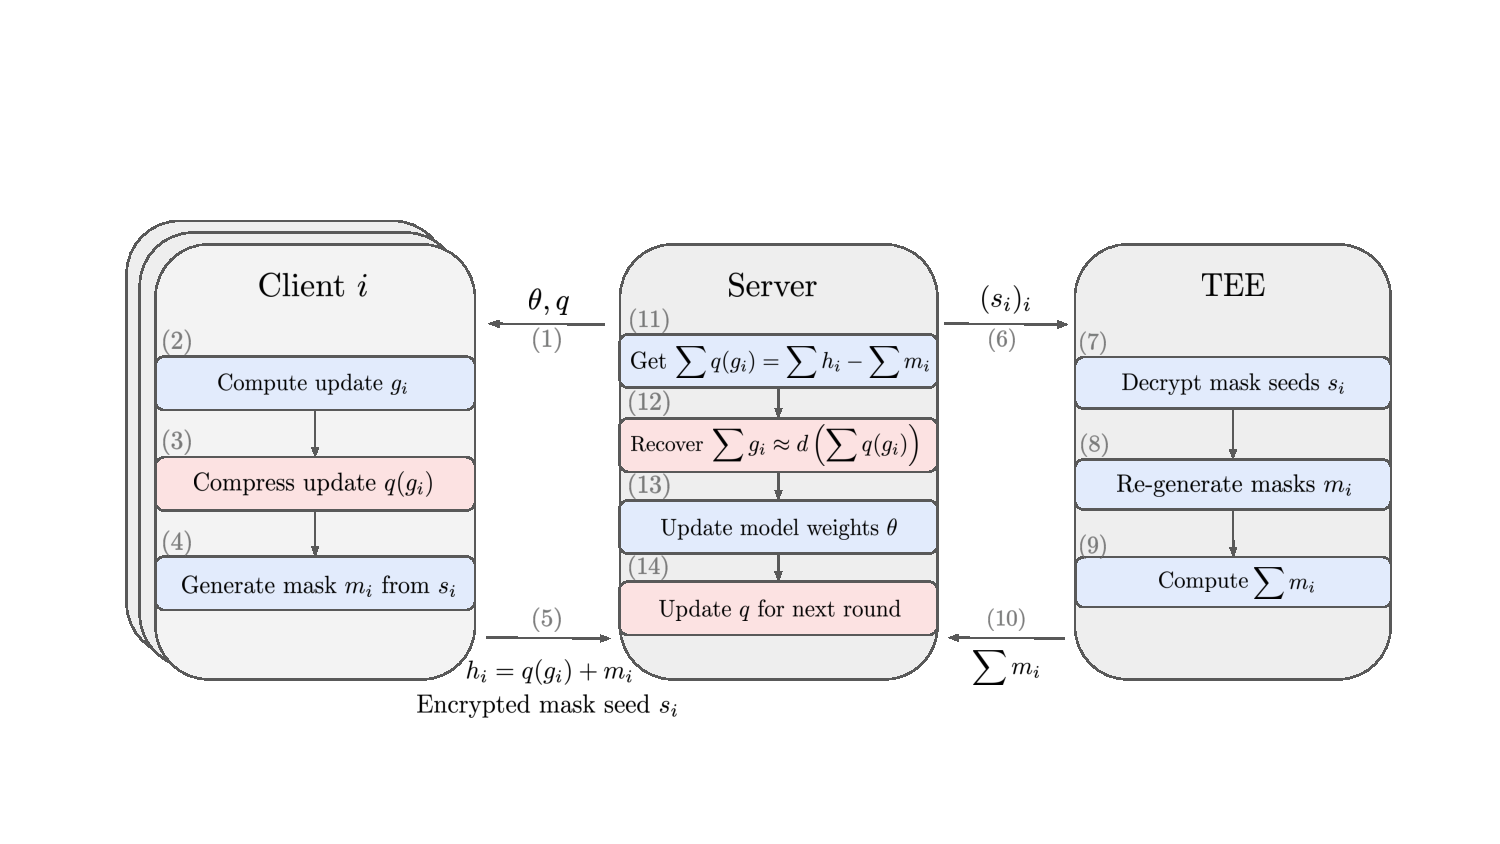
\includegraphics[width=0.8\textwidth]{figs/secagg_summary_new.pdf}
    %\vspace{-5mm}
    \caption{\label{fig:secagg_summary}
    Summary of the proposed approach for one FL round, where we omit the round dependency and \modif{Differential Privacy (DP)} for clarity. Blue boxes denote standard steps and red boxes denote additional steps for uplink compression. Client $i$ computes local model update $g_i$, compresses it with the compression operator $q$, and encrypts it by adding a random mask $m_i$ in the compressed domain, hence reducing the uplink bandwidth (steps 2--4). The server recovers the aggregate in the compressed domain by leveraging any \SecAgg protocol \modif{(steps 7--13, with a TEE-based \SecAgg, see Section~\ref{subsec:secagg})}. Since the decompression operator $d$ is linear, the server can convert the aggregate back to the non-compressed domain, up to compression error (step 12). As with the model weights $\theta$, the compression operator $q$ are also periodically updated and broadcast by the server (step 14). 
    In Section~\ref{sec:method}, we apply the proposed method to scalar quantization and pruning without impacting \SecAgg and propose Secure Indexing, a variant of \SecAgg for extreme uplink compression with product quantization. See Section~\ref{subsec:secagg} for details about \SecAgg and Section~\ref{sec:discussion} for a discussion on~DP.
    }
    \vspace{-3mm}
\end{figure*}



% Our focus in this paper is on 

%Second, scaling cross-device (synchronous) FL to millions of clients with various capabilities and intermittent availability \citep{bonavitz2019federated} suffers from diminishing returns: the wall-clock training time plateaus as the number of clients keeps increasing~\citep{huba2021papaya}. Even though this challenge can be addressed by leveraging the buffered asynchronous aggregation technique proposed by \cite{nguyen2021federated}, compatible with DP and SecAgg, the asynchronous protocol remains bottlenecked by communication latency between the server and the clients.


%Considering the above privacy and scalability goals, we focus on enabling efficient FL communications while keeping a high privacy bar. In addition to the primary objective of speeding up convergence, reducing communication costs brings other significant benefits. Lowering communication requirements addresses selection bias due to undersampling clients with limited connectivity, improving fairness and inclusivity metrics. Better communication efficiency shrinks the carbon footprint of FL, whose fraction attributable to communication can reach 95\%~\citep{qiu2021first}. %Finally, training larger model in FL would be a possibility, when the communication cost is reduced, because local memory or compute requirements can be addressed by modifying the local training loop, for instance with gradient checkpointing \citep{chen2016training}. However, some form of compression would be required to enable efficient communication.


%First, compressing model updates from the client to the server presents several challenges due to compatibility with SecAgg and is an area suitable for further research. 
%Second, upload bandwidth is generally more restricted than download. For instance, according to the most recent FCC report, the ratio of download to upload speeds for DSL/cable providers in the US ranges between 3$\times$ to 20$\times$~\citep{fcc-broadband}. We consider broadband speeds here because devices participate in the FL training while connected to fixed broadband, usually through Wi-Fi~\citep{huba2021papaya}.




% Hence, FL provides the ability to leverage data from massive client populations while ensuring the security and privacy of the client data.
% Go further: compatibility with DP / compression as a mitigation techniques of attacks
% Model and gradient compression intrinsically different.
%  Why not having the secure enclave perform the aggregation?
% \section{Requirements for a Multi-modal Data Science Platform}
\label{sec:requ-holist-data}

In this section we outline the requirements of a multi-modal data science platform and then introduce Vizier as a solution fulfilling these requirements. We start by discussing existing modalities that are widely used to interact with data in data science and their advantages and disadvantages. Converging on a set of modalities we deem to be essential, we then cover several cross-cutting concerns such as reproducibility and dealing with errors that are important no matter what modality is used to interact with data.

%%%%%%%%%%%%%%%%%%%%%%%%%%%%%%%%%%%%%%%%%%%%%%%%%%%%%%%%%%%%%%%%%%%%%%%%%%%%%%%%
\subsection{Modalities for Interacting with Data}
\label{sec:modal-inter-with}

Data scientists often employ several tools during the life-cycle of building a data pipelines. During data discovery, search engines (e.g., open data repositories) and dataset discovery tools (e.g., metadata management tools for data lakes) are used to identify data internal to an organization, data available for purchase, or openly available data that could be used to fulfill the goal the data scientist has in mind. The next step is typically to profile the data and understand its semantics and fitness for the task at hand. At this stage, data visualization is used, either in the form of specialized visualization systems or by employing visualization libraries written in, e.g., Python. This is often done from within notebook environments like Jupyter which can show visualizations inline with the users code. Afterwards, data is curated and integrated. Spreadsheets are often used for manual inspection of smaller datasets, repair of one-off errors, and to calculate basic statistics. Task-specific data cleaning systems or libraries written in a general purpose programming language are employed to (partially) automate this process. The cleaned and integrated data is then used in data analysis (e.g., building and evaluating machine learning models, running analytical queries, \ldots) and the final results of the analysis are visualized. Building a data pipeline is often an iterative process where the user revisits previous steps in the pipeline to deal with errors and to refine the processing.

%%%%%%%%%%%%%%%%%%%%%%%%%%%%%%%%%%%%%%%%%%%%%%%%%%%%%%%%%%%%%%%%%%%%%%%%%%%%%%%%
\subsubsection{Notebooks for Interactive Pipeline Development with Immediate Feedback}
\label{sec:noteb-inter-pipel}
%
Notebook systems like Jupyter and Apache Zeppelin to name just a few have become the quasi-standard for developing data science pipelines. One major advantage of notebooks is their highly interactive nature: users can run pieces of code and immediately observe their results. This makes it easy to debug steps in the pipeline and aids iterative development of pipelines. The outputs recorded in a notebook serve as a documentation of the data preparation and analysis process. Furthermore, most notebook system allow support documentation (typically written in a markup language such as markdown) to be interleaved with code. Even notebook interfaces have become prevalent, most existing implementations are suffer from poor reproducibility, do not support iterative development well, and are not suited well for large and complex pipelines. A recent study~\cite{PM19} on Jupyter notebooks collected from github observed that only 4\% of these notebooks are reproducibly in the sense that they can be rerun without errors and produce the same result as recorded in the notebook. We have argued in \cite{BS20, DG22} that these shortcomings are not inherent to the notebook model, but rather are the result of the architecture of notebook systems which use a long running kernel (e.g., a Python interpreter) and when the user runs a cell in a notebook send the cell's code to the kernel for execution. The kernels state, however, is hidden from the user and except for cell outputs is not encoded in the notebook itself. This leads to unreproducible behavior where the results recorded in the notebook no longer agree with a serial (top-down) execution of the notebook's cells. Furthermore, this can lead to stale results, if the user forgets to rerun cells whose code does dependent on the code in a cell that has been changed. Given the many benefits of and broad use of notebooks, support for a notebook interface is a must for any data science platform. We argue that by providing a notebook interface on top of a specialized workflow engine we can avoid the pitfalls of notebook systems which are thin wrappers around a kernel (Python interpreter). Specifically, we want a solution that supports a notebook interface (\textbf{requirement (N)} which fulfills the following conditions:
\begin{itemize}
\item \textbf{(N1) Serial Execution Semantics:} At any point in time, the results for the cells of the notebook agree with the results produced by a serial execution of the notebook.
\item \textbf{(N2) No Stale Outputs:} The outputs of each cell in the notebook should correctly reflect the current version of the notebook's code.
\item \textbf{(N3) Reproducibility:} The execution of a pipeline (notebook) does not depend on any hidden state. That is, as long as the code in the notebook is deterministic, rerunning a pipeline produces the same output as the original execution.
\end{itemize}

Note that any system that guarantees serial execution of notebooks as defined above, automatically guarantees that there are no stale outputs and that the execution of a notebook is reproducible.


%%%%%%%%%%%%%%%%%%%%%%%%%%%%%%%%%%%%%%%%%%%%%%%%%%%%%%%%%%%%%%%%%%%%%%%%%%%%%%%%
\subsubsection{Spreadsheets for Manual Curation and Exploration}
\label{sec:spre-manu-curat}
%
While notebooks are suited well for programmatic transformation and exploration of data, spreadsheet interfaces enable manual exploration and one-off transformations and fixes~\cite{FG16}. For instance, a user may search for and correct a few mistyped attributes values through a spreadsheet interface. Spreadsheets are also suited well for testing simple data transformations on a few rows using formulas and then once the transformation is satisfactory apply the transformation to a large number of rows by applying the same formula to many rows. Many spreadsheet systems have support for tracking changes made to the spreadsheet, but lack mechanisms to navigate the version history of a spreadsheet and to create branches, e.g., to try out a crazy idea without breaking a deployed version of a data science pipeline. As observed elsewhere~\cite{bendre-19-fhs}, spreadsheet systems do not typically scale to large datasets. While it is anyways infeasible to manually clean and curate large datasets, developing manual fixes on a sample / subset of a large dataset and then deploying the fixes to the dataset can be quite effective. Most spreadsheet systems use a data model that is incompatible with other structured data models such as the relational data model or data frames (which are essentially relations with row indexes) in that (i) columns do not have to be declared but are used by inserting a value into one cell of a column, (ii) the values of a column do not need to belong to a single datatype (e.g., some cells in a column may store strings while others are integers), and (iii) some operations  change the row and column positions rather than their content (e.g., inserting a row, changes the positions of all following rows). To support spreadsheets as a modality (\textbf{requirement (S)}, data science platforms should:
\begin{itemize}
\item \textbf{(S1) Translating between Relations and Spreadsheets:} It should be possible to manipulate standard relations through a spreadsheet view as well as process spreadsheets in other modalities.
\item \textbf{(S2) Supporting Spreadsheet Operations over Relations:} It should be possible to apply spreadsheet operations such as inserting / deleting rows / columns.
\item \textbf{(S3) Scalability:} It should be possible access large datasets through a spreadsheet interface.
\end{itemize}

%%%%%%%%%%%%%%%%%%%%%%%%%%%%%%%%%%%%%%%%%%%%%%%%%%%%%%%%%%%%%%%%%%%%%%%%%%%%%%%%
\subsubsection{Profiling and Interactive Visualizations}
\label{sec:inter-visu}
%
Data profiling and visualization are important tools for data scientists to explore data, understands its semantics, and identify problems with the data.
Data science platforms should support visualizations (\textbf{requirement (V)}). For example, a typical task in the initial data exploration phase of constructing a pipeline is to analyze and visualize the data distributions of columns in a dataset, e.g., by computing histograms for individual columns or by calculating the number of null values per column. Another common approach is to visualize correlations between columns. Both the spreadsheet and notebook modalities discussed so far, do support creation of plots and other data visualizations. Visualization recommendation~\cite{lee-21-l, hu-19-v} guide the user in exploring visualizations that help them to understand their data. A data science platform should support out-of-the-box visualizations  for common tasks (\textbf{requirement (V1)}, e.g., accessing data distributions as histograms as well as provide access to more general visualization tools (\textbf{requirement (V2)} to enable creation of custom visualization of, e.g., analysis results.

%%%%%%%%%%%%%%%%%%%%%%%%%%%%%%%%%%%%%%%%%%%%%%%%%%%%%%%%%%%%%%%%%%%%%%%%%%%%%%%%
\subsubsection{Semi-automated Data Cleaning, Curation, and Integration}
\label{sec:semi-automated-data}
%
As has been observed repeatedly in the past~\cite{nyt:wrangling}, data scientists spend the majority of their time in data discovery, preparation, and curation. Data cleaning, integration, and curation are complex tasks that are time consuming and error-prone. While full automation of these tasks is typically not an option, a plethora of semi-automated tools (e.g., constraint-based data cleaning~\cite{ilyas-15-tcrd}, schema matching~\cite{RB01}, and data integration~\cite{HR06}) which rely on heuristics and often involve the user in curation decisions have been proposed and exist in the form of stand-alone tools and libraries available for languages such as Python. Data science platforms should enable users to use such tools and algorithms in their data science pipelines (\textbf{requirement (C)}. Most approaches for automating data wrangling rely on heuristics to clean data. This is due to the fact that typically insufficient information is available to determine what the correct repair for a dataset is. For instance, when repairing a primary key constraint by tuple deletion~\cite{ilyas-15-tcrd}, one has to retain at most one tuple from each group of tuples with the same primary key value, however, we typically lack information to decide which tuple is the correct one to keep. Thus, data repair algorithms instead use heuristics such as preferring tuples with values that are common in the dataset or optimizing a global metric~\cite{RC17}. Data science platforms should track changes made based on heuristics and how they affect downstream operations as well as provide the user with an overview of what other choices did exist and how different choices would have affected the user's analysis results (\textbf{requirement (U)}):
\begin{itemize}
\item \textbf{(C) (Semi-)automated Data Curation and Integration:} Data science platforms should empower users to access (automated) data curation, cleaning, and integration techniques.
\item \textbf{(U) Tracking the Impact of Uncertain Choices:}  The impact of heuristic choices should be tracked through the operations in a data pipeline to aide the user in understanding how these choices have affected their analysis results and how the results would be affected if another alternative would have been chosen during data cleaning.
\end{itemize}

In summary, all modalities we have discussed so far have in common that they provide ways for the user to interact with data by applying transformations that create new data artifacts or update existing data artifacts and by viewing artifacts through user interfaces. For instance, plotting a histogram of the value distribution of an attribute in a csv file involves several transformations: (i) load the CSV file into a suitable in-memory data structure (e.g., a Pandas dataframe); (ii) aggregate the data to create a histogram; (iii) transform the histogram into a plot. We argue that it is feasible to build multiple modalities as ``views'' on top of a single dataflow platform. This approach has the advantage that the user does not have to to manually transform data between different formats expected by systems implementing the different modalities. Even more important, critical orthogonal functionality  such as versioning (that we will discuss next) has to only be implemented once.

%%%%%%%%%%%%%%%%%%%%%%%%%%%%%%%%%%%%%%%%%%%%%%%%%%%%%%%%%%%%%%%%%%%%%%%%%%%%%%%%
\subsection{Cross-cutting Concerns}
\label{sec:cross-cutt-conc}

Independent of which modality is used to interact with the data, there are important cross-cutting concerns such as reproducibility, supporting the user in iterative development of their data pipelines, dealing with data errors and uncertainty, and how to document data which need to be addressed. Some of the issues with implementing these cross-cutting functionality for specific modalities was already discussing in \Cref{sec:modal-inter-with}, but here we

\begin{itemize}
\item \textbf{(R) Reproducibility and Versioning:} Developing a data science pipeline typically requires several rounds of iterative development and refinement and may involve more than one developer. Keeping track of versions of the pipeline (and the associated results) in a version control manner is critical for aiding users in their development process (e.g., roll back to a past working version of the pipeline or test an experimental idea in a separate branch). However, we argue that unlike in version control systems where the user decides which versions of their code are persisted, for data science platforms it is beneficial if by default all past versions are retained (\textbf{requirement (R1)}). That is there should be no difference between the state kept for supporting undo as well as state kept for versioning. Furthermore, for reproducibility, unless the user's code contains non-deterministic operations, repeated executions of a pipeline should return the same result. Since we want to support interactive modalities like spreadsheets, modifications made through such modalities (e.g., manual edits of cell values or inserting and deleting rows in a spreadsheet) have to be translated into steps in the pipeline (\textbf{requirement (R2)}).
\item \textbf{(I) Supporting Iterative Refinement of Pipelines:} Data pipelines are typically constructed in an iterative fashion by adding additional steps and revisiting prior steps in the pipeline. For example, if an analysis returns unexpected results, the user may backtrack and modify steps in the pipeline which clean the data that is used in the analysis. A data science platform should support users in this process by (i) providing an overview of the structure of the pipeline to help the user to navigate between different parts of the pipeline (\textbf{requirement (O)}), (ii) by providing coarse-grained provenance to help the user identify which steps affected the data used by a pipeline step (\textbf{requirement (P)}), and (iii) ensure that outputs of pipeline steps are always up to date when upstream steps are modified. Note that the last requirement is the ``no stale outputs'' requirement (\textbf{requirement (N2)}) we have already discussed in \Cref{sec:noteb-inter-pipel}.
\item \textbf{(D) Documenting Data and Operations:} One advantage of notebook style interfaces is that they allow code and data to be documented using a markup language. For instance, a user may use this feature to document some insights into the semantics of their data or to explain why they selected a particular cleaning or learning technique. However, documentation in notebooks is associated with steps in the pipeline (cells in the notebook) rather than with pieces of data. While this type of documentation should be support (\textbf{requirement (D1)}), data documentation serves a wide range of purposes such as documenting data semantics (e.g., the year for a column storing dates as a month and day of the month), encoding information of how data was collected and processed, and recording information about issues with the data (e.g., a heart rate measurement is outside of the physically possible range). In \cite{kumari:2021:cidr:datasense} we argued that documentation pertaining to data is mission critical should be associated with the data (\textbf{requirement (D2)}) and should persist through operations (\textbf{requirement (D3)}). For instance, if the user annotated some values in a dataset with a note explaining that these values are suspicious, then aggregated summaries derived from the data should also be associated with these notes.
\item \textbf{(E) Dealing with Errors and Uncertainty:} Uncertainty and errors are prevalent in many application domains due to sensor, outliers~\cite{HA04}, and data entry errors, heuristics applied during data curation, integration~\cite{AS10, FK11b}, and cleaning~\cite{YM15, BS10a}, and misinterpretation of data semantics. Data science platforms should help users in identifying errors, should provide access to semi-automated (heuristic) methods for cleaning and curating data such as the data repair techniques~\cite{B19, ilyas-15-tcrd}. Furthermore, the platform should help the user to determine how choices made during cleaning (whether by a human or an algorithm) affect the results of analyzing the data.
\end{itemize}

In this section we have outlined a set of requirements, both to support specific modalities of interacting with data as well as general requirements that any system for building data science pipelines should support.


%%% Local Variables:
%%% mode: latex
%%% TeX-master: "../2022_IEEE_DEB_Vizier"
%%% End:

%!TEX root=../2022_IEEE_DEB_Vizier.tex

% %%%%%%%%%%%%%%%%%%%%%%%%%%%%%%%%%%%%%%%%
% \begin{figure}[t]
%   \centering
%   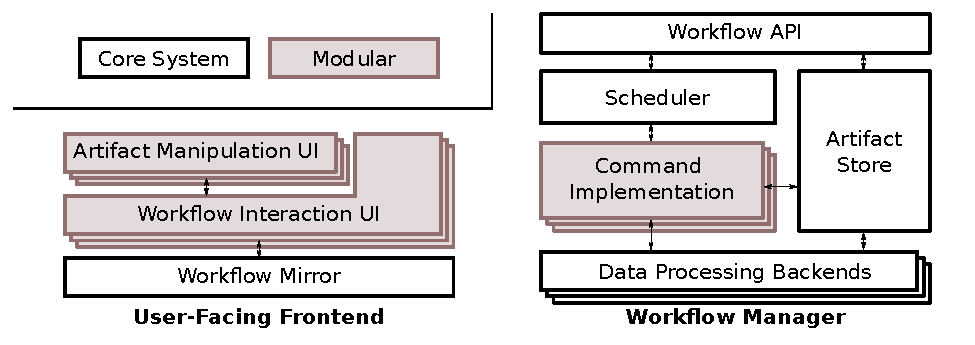
\includegraphics[width=0.7\textwidth]{graphics/systemarch}\\[-5mm]
%   \caption{Vizier's architecture, comprised of a user-facing frontend component and a backend component.}\label{fig:vizier-architecture}
% \end{figure}
% %%%%%%%%%%%%%%%%%%%%%%%%%%%%%%%%%%%%%%%%

%%%%%%%%%%%%%%%%%%%%%%%%%%%%%%%%%%%%%%%%%%%%%%%%%%%%%%%%%%%%%%%%%%%%%%%%%%%%%%%%
\pagebreak[4]
\subsection{Solution Overview}
\label{sec:solution-overview}

%%%%%%%%%%%%%%%%%%%%%%%%%%%%%%%%%%%%%%%%
\begin{wrapfigure}[12]{r}[0pt]{12cm}
  \centering
  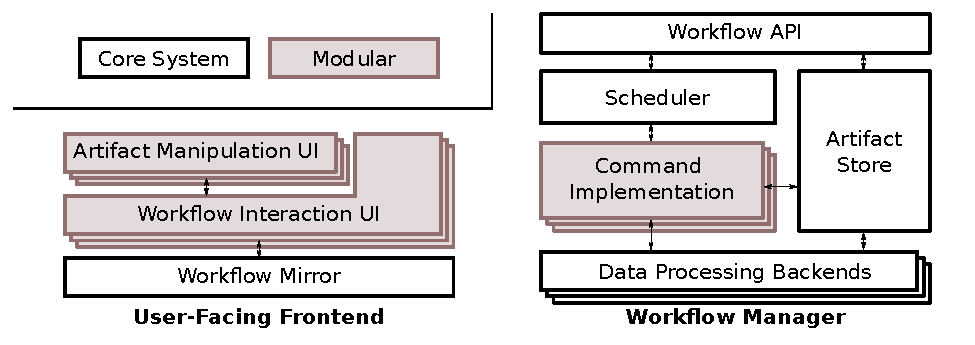
\includegraphics[width=0.7\textwidth]{graphics/systemarch}\\[-5mm]
  \caption{Vizier's architecture, comprised of a user-facing frontend component and a backend component.}\label{fig:vizier-architecture}
\end{wrapfigure}
%%%%%%%%%%%%%%%%%%%%%%%%%%%%%%%%%%%%%%%%
An overview of Vizier's architecture is shown in \Cref{fig:vizier-architecture}.
Addressing requirement \textbf{W1}, the central abstraction in Vizier is a workflow: a linear sequence of steps. % taken by the user in pursuit of a specific objective.
Unlike classical workflow systems, Vizier does not require users to explicitly declare information flow between steps.
Rather Vizier borrows the model employed in popular computational notebooks like Jupyter, where inter-cell communication occurs through a global state (artifacts) passed sequentially through steps.
Following notebook conventions, we refer to these steps as \emph{cells}, and the global state as a \emph{scope}, a map from artifact name to the version of the artifact valid at this point in the workflow. Vizier stores artifacts in common formats through a versioned \textbf{Artifact Store} (\Cref{sec:data-artifacts}), addressing requirement \textbf{A2}.
In \Cref{sec:vizier-workflows}, we formalize Vizier's workflow model, and show how we satisfy requirement \textbf{W3} by instrumenting how each cell interacts with the scope, allowing us to determine what artifact versions are valid.

Vizier's workflow semantics, paired with the versioned artifact store and workflow versioning (\Cref{sec:vizier-history}) addresses requirement \textbf{W2}. % as notebooks have a natural concept of logical order (the order of cells in the notebook) that can be adjusted over time.
% Adding workflow versioning  is sufficient to fully address the requirement.
In contrast, classical notebooks like Jupyter or Zeppelin rely on the global state of an interpreter for inter-cell communication.
Reverting this state to an earlier revision is challenging~\cite{zelnicki:2017:nodebook}, limiting their ability to satisfy requirement \textbf{W3}.
Vizier instead relies on its versioning system, allowing its \textbf{Scheduler} to automatically detect and re-evaluate stale cells (\Cref{sec:vizier-scheduler}).
To address requirement \textbf{A3}, we designed a light-weight uncertain data model that is implemented in Vizier in the form of \textit{caveats}, annotations on data that indicate uncertain values and rows  (\Cref{sec:data-docum-error}).

Addressing requirement \textbf{A1} requires modularity in both Vizier's front- and back-end components.
First, the user's interactions with a workflow and artifacts, whether through a scripting language, graphical interaction, or any other modality, need to be captured for replay (simultaneously addressing requirement \textbf{A4}). In Vizier this is achieved by requiring that every update to an artifact made through a particular modality has to be reflected as an operation in the workflow, i.e., a data update is translated into a workflow update.
Vizier manages a collection of \textbf{Command Implementations} that implement the logic behind these artifact transformations (\Cref{sec:multimodality}).
To streamline the implementation of commands, Vizier's data formats and transformations are built over standard \textbf{Data Processing Backends} like Apache Spark.
% For example, Vizier supports fine-grained provenance over datasets by encoding them as Spark data frames.

The frontend is implemented over a \textbf{Workflow Mirror} that uses websockets to reflect a live view of the workflow the user is editing.
Vizier automatically derives a default \textbf{Artifact Manipulation User Interface} for its notebook interface from each command's parameter schemas. This interface suffices for many templated commands, but the frontend can be further extended to provide a more customized experience, for example for Spreadsheet-style direct manipulation of data (\Cref{sec:spreadsheets}).
As illustrated in \Cref{fig:screenshot}, the frontend displays three \textbf{Workflow Interaction User Interfaces} by default: (i) A direct display of the workflow as a notebook, (ii) a table of contents summary of the notebook, including highlighting from documentation, and (iii) a list of artifacts derived by the notebook.
Several of these components, including the notebook and the artifact list provide access to direct manipulation interfaces.
Additional views currently implemented in Vizier include: (iv) A caveat view (\Cref{sec:data-docum-error}) that shows and tracks potential errors in the workflow and data, (v) a history view that shows the evolution of the workflow over time, and (vi) a data provenance subway diagram view.

%%%%%%%%%%%%%%%%%%%%%%%%%%%%%%%%%%%%%%%%%%%%%%%%%%%%%%%%%%%%%%%%%%%%%%%%%%%%%%%%
\begin{figure}
  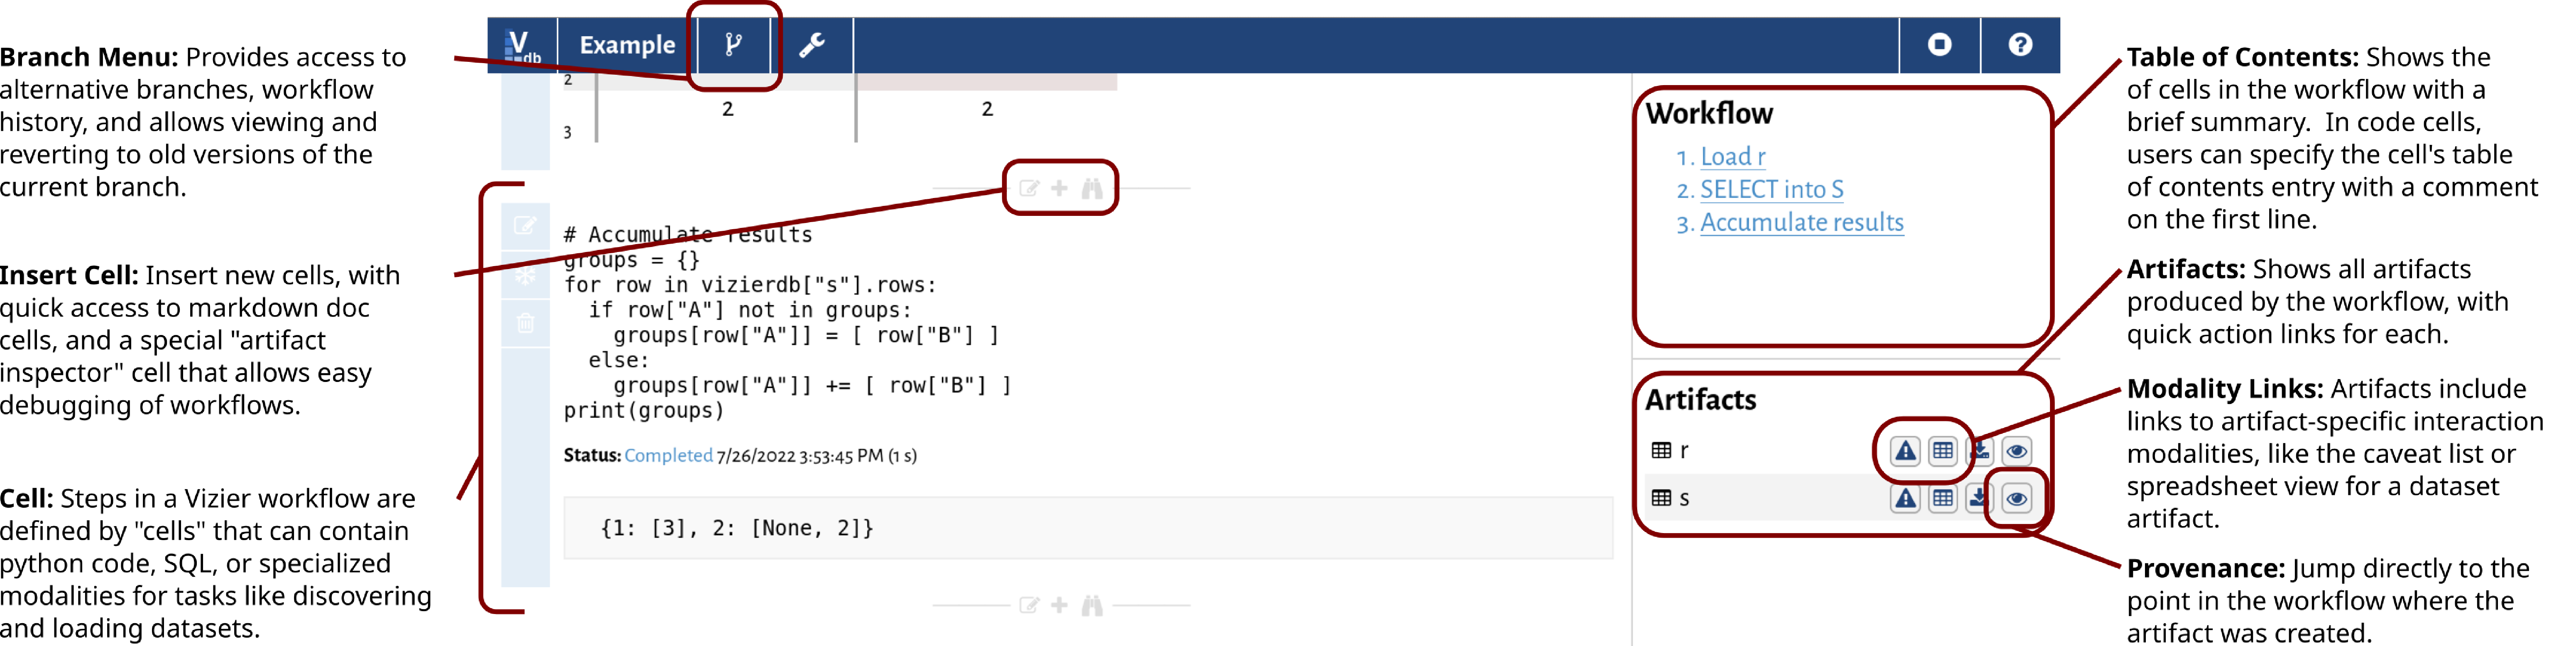
\includegraphics[width=\textwidth]{graphics/screenshot.pdf} 
  \caption{The Vizier User Interface}
  \label{fig:screenshot}
\end{figure}
%%%%%%%%%%%%%%%%%%%%%%%%%%%%%%%%%%%%%%%%%%%%%%%%%%%%%%%%%%%%%%%%%%%%%%%%%%%%%%%%

%%% Local Variables:
%%% mode: latex
%%% TeX-master: "../2022_IEEE_DEB_Vizier"
%%% End:

%!TEX root=../2022_IEEE_DEB_Vizier.tex
%%%%%%%%%%%%%%%%%%%%%%%%%%%%%%%%%%%%%%%%%%%%%%%%%%%%%%%%%%%%%%%%%%%%%%%%%%%%%%%%
\section{Versioned Data Artifact Store}
\label{sec:data-artifacts}

Steps in Vizier workflows create, read, and update \textit{``data artifacts''} or artifacts for short.
To maximize interoperability between cells, Vizier establishes standards for how these artifacts are serialized, which we now discuss. Versions of artifacts are immutable. 
An update to an artifact creates a new object representing the updated artifact. Immutability greatly simplifies handling of state in Vizier and enables us to share artifact versions across multiple revisions of a workflow.

\mypara{Dataset Artifacts}
Tabular data is represented by Vizier as a Spark dataframe~\cite{AX15}, a logical encoding of how a dataset is derived from source data.
The choice to store datasets through a logical representation (specifying the computation instead of its result) is driven largely by the need for managing annotations (requirement \textbf{A3} which is implemented by rewriting the computation to handle annotations), but also results in lower space consumption.
% Because data frames are not serializable, Vizier instead stores dataframe constructors: standardized logic for instantiating a data frame, e.g. by transforming or applying other artifacts.

% Vizier's dataframe constructors are a close analog of SparkML's \texttt{Pipeline}s, which provide a serializable representation of data frame transformation logic.
% Although Vizier provides a pipeline data frame constructor, Pipelines are strictly a representation of transformations, normally requiring glue code to apply the pipeline to an independently loaded dataset;
% Constructors completely capture the logic needed to instantiate a dataframe.

\mypara{Parameter Artifacts}
A parameter artifact can be any primitive value of any data type supported by Apache Spark; We note that this includes simple nested collections like Arrays and Maps.
This type of artifact provides a way to parameterize scripts and other system components, particularly for non-technical users.
% Vizier provides a ``Set Parameter'' command that allows users to specify parameters;
and parameter artifacts are used to pass simple data (e.g., simple constants in Python) between cells.

In addition to these two artifact types, Vizier also supports plots (stored in the vegalite~ \cite{DBLP:journals/tvcg/SatyanarayanMWH17} format), blobs and uninterpreted files, and language-specific constructs, e.g., Python function definitions. For lack of space, we do not further  discuss these other artifact types.

% \mypara{Chart Artifacts}
% Although Vizier provides means for plot generation (e.g., Bokeh, Matplotlib) through messages emitted by a cell, a standardized vegalite~\cite{DBLP:journals/tvcg/SatyanarayanMWH17} artifact format allows multiple cells to collaboratively edit a plot.
% For example, a ``Chart'' command makes it easy for users to quickly visualize a dataset, and then a Spark or Python cell can refine the resulting visualization by tweaking labels, adding markers, or adjusting colors.

% \mypara{Blob and File Artifacts}
% As a fallback to other data formats, Vizier allows cells to export state through a simple blob format.
% For example, Python falls back to encoding global state in `pickle' format, which is stored as a simple blob.
% The blob store is encoded as an in-memory array; If the artifact is large enough to warrant disk IO (e.g., a large model), requires a directory structure (e.g., parquet files), or is otherwise tied to the filesystem, Vizier provide a file artifact format.
% File artifacts are stored in a unique location tied to the artifact identifier.

% \mypara{Function Artifacts}
% Symbols representing language-specific constructs like functions, classes, and imported modules are encoded as raw code.
% Each artifact stores condains code that defines a single symbol under a specific name.
% At time of writing, support for function artifacts requires explicit cross-platform implementation support, although efforts are under way to provide a standardized cross-language interface.




%%% Local Variables:
%%% mode: latex
%%% TeX-master: "../2022_IEEE_DEB_Vizier"
%%% End:

% %!TEX root=../2022_IEEE_DEB_Vizier.tex
\section{Microkernel Notebooks}
As we outline above, a typical computational notebook relies on a kernel, a long-lived interpreter for a scripting language for a scripting language like python that retains the notebook's intermediate state.
When a cell is executed by the user, its contents are evaluated by the long running interpreter; the interpreter's state changes, and any output produced by the cell (e.g., console logs, charts, or maps) is displayed alongside the cell.
This behavior is independent of the order in which the cell appears in the notebook: The user may return to an earlier cell and modify it, but this cell is simply run against the current state of the interpreter.

Although this design allows users to revise cells in the notebook without being forced to re-run all of the notebooks code from scratch, it does pose several problems.
Most notably that it forces users to reason about the internal state of the kernel, for example by manually adopting a single static assignment variable allocation pattern.
Second, it also requires users to manually keep track of how different notebook cells relate to one-another; When a cell is modified, other cells that depend on it may also need revision.
Finally, in this design, persistence (e.g., of the results of a slow-running computation) must be managed entirely by the user.
Moreover, it is up to the user to manually manage this state to ensure consistent versioning, and portability.

One class of systems including Vizier~\cite{BS20,BB19} and Nodebook address these challenges by checkpointing global notebook state in between cell executions and restoring it when a cell is re-executed.
Thus, the cell is always evaluated on the state version emitted by the preceding cell, and changes to the state can be identified so that subsequent cells that depend on modified outputs can be re-evaluated.
This model 


\begin{itemize}
	\item Standard API for interacting with notebook state facilitates multi-modality
	\begin{itemize}
		\item No $N^2$ problem like for jupyter kernels
		\item Not just notebooks
	\end{itemize}
	\item Typed API allows fine-grained provenance
	\begin{itemize}
		\item Reproducibility
		\item Automatic refresh
		\item No hidden (mystical) dependencies
	\end{itemize}
	\item Challenges:
	\begin{itemize}
		\item Communicating state between kernels
		\item 2-dimensional version model (cell-order vs historical-order <- better name for this exists)
		\item Input/output changes in history vs Operation changes in history
		\begin{itemize}
			\item Vizier: Module vs Cell vs Result
			\item The Vizier execution state-model
		\end{itemize}
		\item Scheduling / Deciding state
	\end{itemize}
\end{itemize}

%%% Local Variables:
%%% mode: latex
%%% TeX-master: "../2022_IEEE_DEB_Vizier"
%%% End:

%!TEX root=../2022_IEEE_DEB_Vizier.tex
\section{Workflow Provenance Model and Runtime}
\label{sec:vizier-workflows}

In this section, we outline Vizier's workflow and versioning model, how we determine which cells of a workflow need to be re-executed if a cell is changed, and introduce the parallel scheduler of the system.

% multi-tiered, two-dimensional provenance model.
% We first relate the model to both classical workflow provenance and modern computational notebooks, then discuss how Vizier's model incorporates a temporal dimension, and finally discuss state invalidation and re-evaluation.

\newcommand{\notebook}{\mathcal N}
\newcommand{\workflow}{\mathcal W}
\newcommand{\artifact}{a}
\newcommand{\nbcell}{c}
\newcommand{\outputval}{o}
\newcommand{\readset}{\vec r}
\newcommand{\writeset}{\vec w}
\newcommand{\globalscope}{\mathcal G}
\newcommand{\outputdomain}{\mathcal O}
\newcommand{\valuedomain}{\mathcal D}
\newcommand{\undefinedval}{\bot}
\newcommand{\unknownval}{\circledcirc}
\newcommand{\keyset}{\texttt{keys}}
\newcommand{\changeset}{\Delta}
\newcommand{\variabledomain}{\Sigma}
\newcommand{\diff}[2]{\Delta(#1, #2)}
\newcommand{\evalnb}[1]{\llbracket #1 \rrbracket}

\begin{figure}
  \centering
  \begin{minipage}{0.9\textwidth}
  \begin{lstlisting}[style=pynotebook]
data = read_csv("social_data.csv")
show(data)
  \end{lstlisting}

  \begin{lstlisting}[style=pynotebook]
data["latlon"] = geocode(data["address"])
show(data)
  \end{lstlisting}

  \begin{lstlisting}[style=pynotebook]
censusblocks = read_geojson("blocks.json")
show(censusblocks)
  \end{lstlisting}

  \begin{lstlisting}[style=pynotebook]
data = spatial_join(data, censusblocks, ["latlon", "geometry"])
count_per_block = data.groupby("block_id").count()
show(count_per_block)
  \end{lstlisting}
  \end{minipage}\\[-4mm]
  \caption{A simplified example notebook}
  \label{fig:exampleNotebook}
\end{figure}

%%%%%%%%%%%%%%%%%%%%%%%%%%%%%%%%%%%%%%%%%%%%%%%%%%%%%%%%%%%%%%%%%%%%%%%%%%%%
%%%%%%%%%%%%%%%%%%%%%%%%%%%%%%%%%%%%%%%%%%%%%%%%%%%%%%%%%%%%%%%%%%%%%%%%%%%%
\subsection{Workflow Model}
\label{sec:vizier:eval}

A workflow in Vizier is a sequence of workflow steps (cells) that can read and write artifacts. 
Artifacts are versioned at the granularity of cells. 
A cell writing an artifact $\artifact$ causes a new version of $\artifact$ to be created. 
We will discuss the APIs Vizier exposes to the data interaction modalities for accessing artifacts in \Cref{sec:multimodality}. 
The semantics of a Vizier workflow is the serial execution of the cells of the workflow, where the latest version of each artifact is passed as input to the cell that will be executed next. 
Thus, as long as the cells themselves are deterministic, the artifact versions created by the execution of a workflow are uniquely determined by the workflow itself.

%%%%%%%%%%%%%%%%%%%%%%%%%%%%%%%%%%%%%%%%%%%%%%%%%%%%%%%%%%%%%%%%%%%%%%%%%%%%%%%%
\begin{exam}
  \label{ex:introduction}
  \Cref{fig:exampleNotebook} shows a notebook with a simplified data ingestion, cleaning, and analysis task.
  The notebook loads the dataset (cell 1), geocodes listed street addresses (cell 2), loads a collection of census blocks (cell 3), and computes summary statistics for each census block (cell 4).
  We use this  notebook to illustrate a key challenge of traditional  notebook architectures.
  %
  The user modifies cell 2 to switch to a different geocoder, potentially requiring re-evaluation of the notebook.
  In this specific notebook, the user had the foresight to write in an idempotent style, making it unnecessary to re-run cell 1 to recover the state needed to run cell 2 correctly.
  It is also unnecessary to re-run cell 3, as it does not depend on the output of cell 2.
  However, in traditional notebooks like Jupyter the burden of deciding which cells to re-evaluate rests on the user, creating added overhead and increasing the chance of errors.
\end{exam}
%%%%%%%%%%%%%%%%%%%%%%%%%%%%%%%%%%%%%%%%%%%%%%%%%%%%%%%%%%%%%%%%%%%%%%%%%%%%%%%%

Formally, a Vizier workflow is a sequence $\notebook = \{ \nbcell_1, \ldots, \nbcell_N \}$ of cells. 
The versions of artifacts valid after execution of cell $\nbcell_i$ are modeled as a global scope $\globalscope$ that maps artifact names to artifact versions or the distinguished symbol $\undefinedval$, which indicates that no version of the artifact has been produced yet.  
A cell $\nbcell$ is a function that takes a scope $\globalscope$ as input and produces an updated scope $\globalscope'$: $\nbcell (\globalscope) = \globalscope'$. 
We use $\readset_{\globalscope,i}$ to denote the names of artifacts accessed by cell $\nbcell_i$ applied to $\globalscope_i$. 
The scope parameter is necessary, because a cell may dynamically decide which artifacts to read based on the content of other artifacts.
%
The result $\evalnb{\notebook}$ of  evaluating workflow $\notebook = \{ \nbcell_1, \ldots, \nbcell_N \}$ is defined as the scope $\globalscope_n$ produced by starting with an empty scope $\globalscope_0$ (where all artifact names are mapped to $\undefinedval$), and by computing $\globalscope_{i} = \nbcell_{i}(\globalscope_{i-1})$.








% Cell evaluation in Vizier happens in notebook-order.

% Each cell is (conceptually) evaluated on the scope emitted by the preceding cell.
% Like the workflow systems that inspired it, Vizier retains inter-cell snapshots of scope to preserve notebook-order evaluation semantics while still allowing users to backtrack.


% Denote by $\globalscope$ a global scope that we will formalize shortly;

% We model a cell $\nbcell (\globalscope) = (\globalscope', \readset, \outputval)$ as a deterministic function applied to a global scope that returns a new global scope $\globalscope'$, a read set $\readset$, and an opaque output object $\outputval$ in $\outputdomain$.
% Evaluating the notebook $\evalnb{\notebook} = (\globalscope_N, [\outputval_1, \ldots, \outputval_N)$ produces a final scope $\globalscope_N$ and a sequence of outputs $\outputval_1, \ldots, \outputval_N$ through straightforward composition, starting with an empty scope $\globalscope_0$.
% %  formalized as:
% % $$(\globalscope_i, \readset_i, \outputval_i) = \nbcell_i(\globalscope_{i-1})$$
% % In the above,

%%%%%%%%%%%%%%%%%%%%%%%%%%%%%%%%%%%%%%%%
\begin{wrapfigure}[8]{r}[0pt]{11cm}
  \centering
  \vspace{-4mm}
  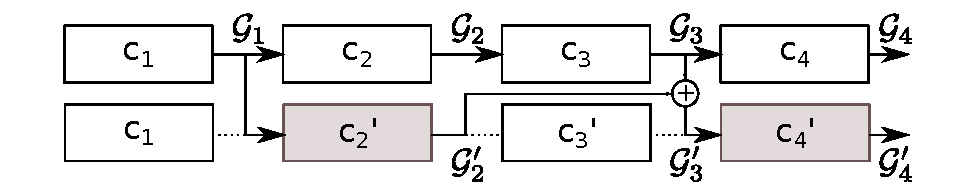
\includegraphics[width=10.5cm]{graphics/eval.pdf}\\[-5mm]
  \caption{Evaluation logic for the example notebook in \Cref{fig:exampleNotebook}.  Edges are labeled with global scope versions.  Cells that are (re-)evaluated are highlighted, dotted lines represent simulated state flow.}
  \label{fig:exampleEval}
\end{wrapfigure}
%%%%%%%%%%%%%%%%%%%%%%%%%%%%%%%%%%%%%%%%
If workflow $\notebook$ is modified by replacing a cell $\nbcell_i$ with a cell $\nbcell_i'$ (denoted as $\notebook[\nbcell_i \backslash \nbcell_i']$), we need to obtain the updated scope $\evalnb{\notebook[\nbcell_i \backslash \nbcell_i']}$. Of course this can be achieved by evaluating $\notebook[\nbcell_i \backslash \nbcell_i']$.
% In lieu of naively re-evaluating the notebook from scratch,
However, to improve performance,  Vizier attempts to update the output of $\evalnb{\notebook}$ by only re-evaluating a subset of the cells.
First, observe that $\globalscope_1, \ldots, \globalscope_{i-1}$ are independent of $\nbcell_i$; and remain unchanged if $\nbcell_i$ is modified.
It is still necessary to have $\globalscope_{i-1}$ to evaluate $\nbcell_i'$; so Vizier caches all intermediate global scopes after evaluating each workflow revision.

% \begin{figure}
%   \centering
%   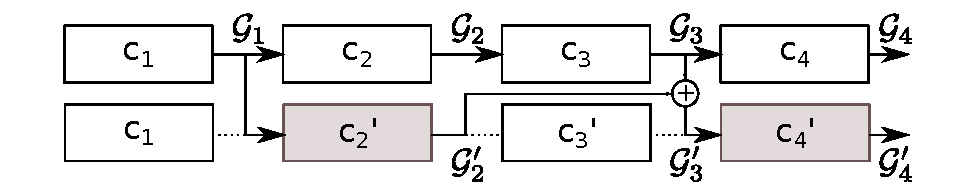
\includegraphics[width=0.7\textwidth]{graphics/eval.pdf}
%   \caption{Evaluation logic for the example notebook in \Cref{fig:exampleNotebook}.  Edges are labeled with global scope versions.  Cells that are (re-)evaluated are highlighted, dotted lines represent simulated state flow.}
%   \label{fig:exampleEval}
% \end{figure}

Naively, we have to still re-evaluate $\nbcell_{i+1}, \ldots, \nbcell_{N}$ using the new scope produced by $\nbcell_i'$. Let us denote the scopes produced by this evaluation as
$\globalscope_{i+1}', \ldots, \globalscope_{n}$.
% $\outputval_{i+1}', \ldots, \outputval_{N}'$.
Vizier uses the readsets $\readset_{\globalscope, i+1}, \ldots, \readset_{\globalscope, N}$, to identify cells $\nbcell_{j}$ for which the same output (artifact versions written by the cell) in $\evalnb{\notebook[\nbcell_i \backslash \nbcell_i']}$ is guaranteed. 
Denote by $\changeset(\globalscope, \globalscope') = \{ k |  \globalscope(k) \neq \globalscope'(k)\}$ the names of artifacts that differ between $\globalscope$ and $\globalscope'$. 
We have to re-execute cell $\nbcell_{i+1}$ if an artifact read by $\nbcell_{i+1}$ has changed, which is the case if $\changeset(\globalscope_i, \globalscope_i') \cap \readset_{\globalscope,i+1} \neq \emptyset$. If $\nbcell_{i+1}$ needs to be re-executed, then we set $\globalscope_{i+1}' = \nbcell_{i+1}(\globalscope_{i}')$. Otherwise, we generate $\globalscope_{i+1}$ by merging the changes made by $\nbcell_{i+1}$ in $\notebook$ to $\globalscope_{i}$ into $\globalscope_{i}'$. That is, for all artifacts $k$ we set
$\globalscope_{i+1}'(k) =   \globalscope_{i+1}(k)$ if $k \in \changeset(\globalscope_i, \globalscope_{i+1})$
and $\globalscope_{i+1}'(k) = \globalscope_{i}'(k)$ otherwise.
% begin{cases}
%   \globalscope_{i+1}(k) &\;\;\;\text{\textbf{if}}\,k \in \changeset(\globalscope_i, \globalscope_{i+1})\\
%   \globalscope_{i}'(k) &\;\;\;\text{\textbf{otherwise}}\\
% \end{cases}$$
 The same approach is applied to decide whether to evaluate or skip the remaining cells in $\notebook[\nbcell_i \backslash {\nbcell_i}']$.


% We formalize a global scope $\globalscope = \{ k_1 \rightarrow v_1, k_2 \rightarrow v_2, \ldots \}$ as a total mapping from an infinite alphabet of variable names $k \in \variabledomain$ to a set of domain values $v \in \valuedomain \cup \{\undefinedval\}$.
% The distinguished symbol $\undefinedval$ denotes an ``undefined'' value, and we assume that finitely many elements of $\variabledomain$ are mapped to non-$\undefinedval$ values (i.e., that $\globalscope$ has finite support).
% Denote by $\keyset(\globalscope) = \{ k | (k \rightarrow v) \in \writeset \wedge v \neq \undefinedval\}$ the keys of the finite support of $\globalscope$.
% Denote by $\changeset(\globalscope, \globalscope') = \{ k |  \globalscope(k) \neq \globalscope'\}$ the change set between $\globalscope$ and $\globalscope'$.

% Given the newly computed $\globalscope_i'$, we want to know if $\nbcell_{i+1}$ needs to be evaluated as well;
% If $\nbcell_{i+1}(\globalscope_i') = (\globalscope_{i+1}', \readset_{i+1}', \outputval_{i+1}')$, we can avoid re-evaluating $\nbcell_{i+1}$ if we can prove that $\outputval_{i+1} = \outputval_{i+1}'$.
% Under the assumption that $\nbcell_{i+1}$ is deterministic with respect to inputs $\readset_{i+1}$, we can guarantee that $\outputval_{i+1} = \outputval_{i+1}'$ when $\readset_{i+1} \cap \changeset(\globalscope_{i}, \globalscope_{i}')$ is empty.
% If we do not need to re-evaluate $\nbcell_{i+1}$, we can reconstruct its output by considering how the original evaluation affected the scope: the write set $\writeset_{i+1} = \changeset(\globalscope_{i}, \globalscope_{i+1})$.
% Concretely $\outputval_{i+1}' = \outputval_{i+1}$, $\readset_{i+1}' = \readset_{i+1}$ and
% $$\globalscope_{i+1}'(k) = \begin{cases}
% \globalscope_{i+1}(k) \textbf{ if } k \in \writeset_{i+1}\\
% \globalscope_{i}'(k) \textbf{ otherwise}
% \end{cases}$$
% \noindent The remaining cells of the notebook are processed in a like manner.

 %%%%%%%%%%%%%%%%%%%%%%%%%%%%%%%%%%%%%%%%%%%%%%%%%%%%%%%%%%%%%%%%%%%%%%%%%%%%%%%%
\begin{exam}
  \Cref{fig:exampleEval} continues the running example from \Cref{ex:introduction}.
  The user has replaced the initial version of cell $\nbcell_2$ with an updated version ${\nbcell_2}'$.
  The global scope produced by preceding cells ($\globalscope_1$) may be re-used unchanged to evaluate ${\nbcell_2}'$, producing scope $\globalscope_2'$.
  $\changeset(\globalscope_2, \globalscope_2')$ is the \lstinline{data} artifact, but the readset of $\nbcell_3$ is empty, and so this cell does not need to be re-evaluated.
  Instead $\globalscope_3'$ is derived by merging variables the cell previously changed (i.e., $\changeset(\globalscope_2, \globalscope_3)$) into the current global scope.
  Finally, Vizier identifies that an element of $\readset_{\globalscope,4}$ (the \lstinline{data} variable) has changed between $\globalscope_3$ and $\globalscope_3'$, necessitating a re-evaluation of cell 4.
\end{exam}
 %%%%%%%%%%%%%%%%%%%%%%%%%%%%%%%%%%%%%%%%%%%%%%%%%%%%%%%%%%%%%%%%%%%%%%%%%%%%%%%%

% \mypara{Frozen Cells}
% Vizier allows users to ``freeze'' cells, temporarily replacing them with no-op commands, but preserving all user-interface elements (including cell outputs), and allowing the cell to be easily re-inserted into the notebook.
% This allows users to quickly disable cells with transient purposes (e.g., sampling cells), or avoid triggering expensive computations while working on an earlier part of the notebook.

% \begin{figure}
%   \centering
%   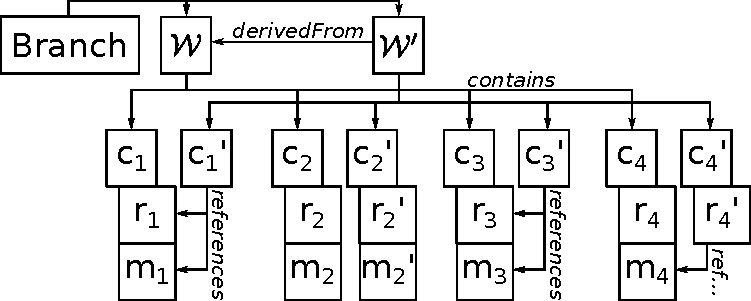
\includegraphics[width=0.45\textwidth]{graphics/history.pdf}\\[-3mm]
%   \caption{History for the running example, assuming cell B was changed as in \Cref{fig:exampleEval}.}
%   \label{fig:exampleHistory}
% \end{figure}

%%%%%%%%%%%%%%%%%%%%%%%%%%%%%%%%%%%%%%%%%%%%%%%%%%%%%%%%%%%%%%%%%%%%%%%%%%%%
%%%%%%%%%%%%%%%%%%%%%%%%%%%%%%%%%%%%%%%%%%%%%%%%%%%%%%%%%%%%%%%%%%%%%%%%%%%%
\subsection{Versioning Workflows}
\label{sec:vizier-history}

%%%%%%%%%%%%%%%%%%%%%%%%%%%%%%%%%%%%%%%%
\begin{wrapfigure}[10]{r}[0pt]{8cm}
  \centering
  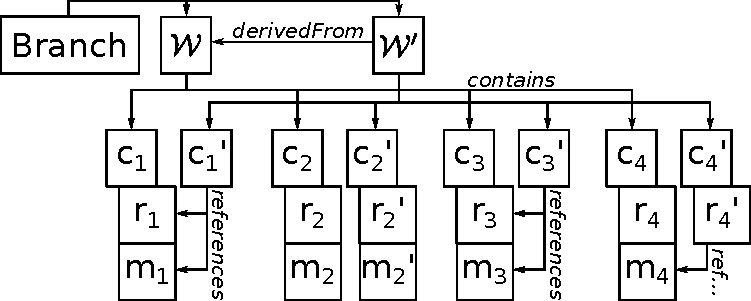
\includegraphics[width=0.45\textwidth]{graphics/history.pdf}\\[-3mm]
  \caption{History for the running example, assuming cell 2 was changed as in \Cref{fig:exampleEval}.}
  \label{fig:exampleHistory}
\end{wrapfigure}
%%%%%%%%%%%%%%%%%%%%%%%%%%%%%%%%%%%%%%%%
Vizier maintains a branching history of the evolution of the notebook.
% We use the term workflow ($\workflow = c_1, \ldots, c_N$) to denote a single state of the notebook.
A cell is further subdivided into (i) \textbf{cell metadata} ($c_i$) that is unique to the workflow (e.g., timestamps and execution status), (ii) \textbf{results} ($r_i$) of executing the cell, and (iii) a \textbf{module} ($m_i$) describing the command executed in the cell.
The latter two components (results and modules) may be shared across workflows.
% In other words, a single cell object acts as a many-to-many-to-many (i.e., 3-ary) relationship between workflow, module, and result entities.
A module object describes the command to be evaluated in a cell.  
This includes its type (e.g., Python or Scala script; SQL query; or one of the graphical widgets), as well as any parameters to the command (e.g., the script itself, or the artifact name to materialize query results as). 
A results object stores references to versions of artifacts in the artifact store created by the execution of the cell. 
We do not materialize the full global scope after each cell, but rather only the changes made to the global scope by the cell (i.e., the cell's write set). 
Any global scope $\globalscope_i$ can be reconstructed from the preceding write sets.

% A results object consists of three items: (i) Messages output by the cell (i.e., $\outputval$), (ii) The cell's readset as a list of name/artifact pairs, and (iii) The cell's writeset as a list of name/artifact pairs.
% Deletion is encoded by writing the distinguished value \texttt{null} to a name.
% As a performance optimization, name/artifact pairs do not embed the artifact literal, but rather a unique artifact identifier.
% This allows for efficient equivalence testing, while avoiding duplication; For example, a ``copy artifact" instruction only needs to clone the artifact identifier under a new name, and not the entire artifact.

% \mypara{Global scope}
% Note that the organizational structure used to persist history information differs from the global scope model used to reason about cell re-use.
% However, the two representations are equivalent.
% Denote by $m_1 \circ m_2$ the right-preferenced composition of \emph{partial} maps $m_1$ and $m_2$ as follows:
% $$m_1 \circ m_2 = \{ k\rightarrow v | (k \rightarrow v) \in m_1 \wedge \not\exists v' \text{ s.t. } (k \rightarrow v') \in m_2 \} \cup m_2$$
% Any global scope $\globalscope_N$ can be recovered by composing the preceding writesets: $\globalscope_N = \globalscope_0 \circ \writeset_1 \circ \ldots \circ \writeset_N$


\begin{exam}
 \Cref{fig:exampleHistory} continues our running example, which in our new terminology is a single branch comprised of two workflows $\workflow_1$ and $\workflow_2$.
  Both notebooks are comprised of four cell objects each.
  Cells 1, 3, and 4 were unchanged between workflows, and so the corresponding cell objects for $\workflow_2$ reference the same module description object as the corresponding cell for $\workflow_1$, while the module descriptions referenced by $\nbcell_2$ and ${\nbcell_2}'$ differ.
  Cells 1 and 3 do not need to be re-evaluated, and so can share their result objects, while Cells 2 and 4 both require re-evaluation and create new result objects.
\end{exam}

%%%%%%%%%%%%%%%%%%%%%%%%%%%%%%%%%%%%%%%%%%%%%%%%%%%%%%%%%%%%%%%%%%%%%%%%%%%%%%%%
\mypara{Workflow and Branch History}
Similar to version control systems like git, each workflow version in Vizier stores a reference to the workflow version it was derived from.
% The difference between workflow versions can be computed by comparing the sequence of modules referenced by the workflow's cells; but simple summary information including the type of change (insert, delete, update) and the affected module (if appropriate) is cached with the workflow object.
A branch is an append-only sequence of workflow versions. % with associated metadata (e.g., a branch name).
The branch contains a reference to the most recent workflow version in the branch. % prior versions are tracked through the series of derived-from references in the workflows themselves.
A new branch may be created from any existing workflow version, including a historical one.

%%%%%%%%%%%%%%%%%%%%%%%%%%%%%%%%%%%%%%%%%%%%%%%%%%%%%%%%%%%%%%%%%%%%%%%%%%%%
%%%%%%%%%%%%%%%%%%%%%%%%%%%%%%%%%%%%%%%%%%%%%%%%%%%%%%%%%%%%%%%%%%%%%%%%%%%%
\subsection{Parallel Scheduler}\label{sec:vizier-scheduler}

The evaluation model presented in \Cref{sec:vizier:eval} relies exclusively on \textit{dynamic provenance}, where Vizier is informed about the readset and writeset of a cell at runtime when the cell accesses artifacts through Vizier's API.
% that assist in determining whether a cell needs to be re-evaluated.
However, dynamic provenance is not always sufficient.
For example, Vizier evaluates cells in parallel where possible, but dynamic provenance is not available until the cell has already been evaluated.
Static provenance, which can derive a cell's read and write sets through static dataflow analysis of its source code, can be computed upfront.
However, static dataflow analysis is of necessity an approximation for some cell types; language features like control flow and dynamic code evaluation can lead to over- (or under-) estimates of the cell's read and write sets. % , especially with respect to a specific global scope.
Vizier uses a novel approach which refines static provenance at runtime using dynamic provenance~\cite{DG22}.

Fundamentally, Vizier's scheduler needs to assign each cell in a running workflow to one of four lifecycle stages: (i) \textbf{DONE} when the cell has a valid result object, (ii) \textbf{PENDING} when the cell depends (directly or transitively) on a cell that does not have a result object, and (iii) \textbf{RUNNING} when the cell's dependencies have a valid result object but the cell itself does not.
We further distinguish as (iv) \textbf{STALE} those cells in the \textbf{PENDING} stage for which we can conclusively determine that re-evaluation is required.
% Lifecycle stage transitions are monotonic.

To manage lifecycle transitions, Vizier's scheduler relies on a combination of static and dynamic provenance~\cite{DG22}.
It uses static provenance to generate an over-approximation on the read and write dependencies of a cell\footnote{As we argue in~\cite{DG22}, to deal with languages that support dynamic code evaluation such as Python, it would be necessary to allow under-approximations of read and write sets (missed data dependencies) and compensate for them at runtime. However, this not implemented in Vizier yet; attempts to dynamically read variables not in the maximal readset are flagged as errors.}.
  % Vizier does not presently support purely dynamic dependencies through e.g., dynamic code evaluation.  A read or write access on a variable not discovered through static analysis triggers an execution error.}.
Accordingly, the scheduler tracks an over-approximation of the read and writesets at each step of the workflow, and refines them when the execution of cell finishes and we know its precise read and write set. 
This approximation is used by Vizier's scheduler to omit cells from re-execution or schedule them for parallel execution if we can determine that it is safe to do so based on these over-approximations.

% Approximate global scopes generalize our prior definition of a global scope by extending the value domain to include the value $\unknownval$, denoting an unresolved value (i.e. variables in an approximate global scope are drawn from $\valuedomain \cup \{\undefinedval, \unknownval\}$).
% Like a regular global scope, an approximate global scope is derived by concatenating writesets ($\globalscope_i = \globalscope_{i-1} \circ \writeset_i$).
% However, if the cell is in a lifecycle stage other than \textbf{DONE}, its previous writeset is not valid.
% Instead, Vizier uses static analysis to derive an upper bound on the writeset $\writeset_{\max} \subseteq \variabledomain$, the maximal set of variables that the cell is allowed to write to.
% When the cell's writeset is not (or may not be) valid, the approximate global scope is instead updated by making each element of $\writeset_{\max}$ an unknown:
% $\globalscope_{i} = \globalscope_{i-1} \circ \{ k \rightarrow \unknownval | k \in \writeset_{\max, i} \}$

% \Cref{alg:lifecycleStage} explains how Vizier derives the lifecycle stage of a cell from the global scope emitted by the preceding cell, the cell's readset (if it exists), and the bound on the readset derived from static analysis.
% The first consideration is whether the cell's prior result object is still valid.
% If there is no prior result object (e.g., because the cell is newly inserted), or if the prior result object is definitely invalid (i.e., because a previously read value was definitely overwritten by a re-evaluated cell), the cell must be re-evaluated.
% What remains is whether the cell can be immediately evaluated (all variables in the upper bound on the readset are defined), or not.

% \begin{algorithm}
% \caption{\lstinline{lifecycle_stage}($\globalscope$, $\readset$, $\readset_{\max}$)}
% \label{alg:lifecycleStage}
% \begin{algorithmic}
%   \REQUIRE{$\globalscope$: The approximate global scope from the prior cell.}
%   \REQUIRE{$\readset$: Either a partial map from $\variabledomain$ to $\valuedomain$ denoting the actual read set if one exists, or $\unknownval$ if the cell is new.}
%   \REQUIRE{$\readset_{\max}$: A set over $\variabledomain$, denoting the statically derived upper bound on the cell's read set.}
%   \ENSURE{$\ell$: The current lifecycle stage of the cell.}
%   \IF{$\readset = \unknownval$ or there exists a $(k \rightarrow v) \in \readset$ such that $\globalscope(k) \neq \unknownval$ and $\globalscope(k) \neq v$}
%     \IF{there exists a $k \in \readset_{\max}$ such that $\globalscope(k) = \unknownval$}
%       \STATE $\ell = \textbf{STALE}$
%         \COMMENT{The cell needs to be re-evaluated, but is missing a dependency}
%     \ELSE
%       \STATE $\ell = \textbf{RUNNING}$
%         \COMMENT{The cell needs to be re-evaluated, and is ready to run}

%     \ENDIF
%   \ELSIF{there exists a $(k \rightarrow v) \in \readset$ where $\globalscope(k) = \unknownval$}
%     \STATE $\ell = \textbf{PENDING}$
%       \COMMENT{The cell may not need re-evaluation, but we don't know yet.}
%   \ELSE
%     \STATE $\ell = \textbf{DONE}$
%       \COMMENT{We can guarantee that the cell does not need re-evaluation.}
%   \ENDIF
% \end{algorithmic}
% \end{algorithm}

% When a cell transitions into the \textbf{RUNNING} state, the scheduler starts the corresponding cell.
% When the cell finishes, it has a state that matches the preceding global state, and transitions into the \textbf{DONE} state.

%%% Local Variables:
%%% mode: latex
%%% TeX-master: "../2022_IEEE_DEB_Vizier"
%%% End:
% %!TEX root=../2022_IEEE_DEB_Vizier.tex
\section{Microkernel Notebooks}
As we outline above, a typical computational notebook relies on a kernel, a long-lived interpreter for a scripting language for a scripting language like python that retains the notebook's intermediate state.
When a cell is executed by the user, its contents are evaluated by the long running interpreter; the interpreter's state changes, and any output produced by the cell (e.g., console logs, charts, or maps) is displayed alongside the cell.
This behavior is independent of the order in which the cell appears in the notebook: The user may return to an earlier cell and modify it, but this cell is simply run against the current state of the interpreter.

Although this design allows users to revise cells in the notebook without being forced to re-run all of the notebooks code from scratch, it does pose several problems.
Most notably that it forces users to reason about the internal state of the kernel, for example by manually adopting a single static assignment variable allocation pattern.
Second, it also requires users to manually keep track of how different notebook cells relate to one-another; When a cell is modified, other cells that depend on it may also need revision.
Finally, in this design, persistence (e.g., of the results of a slow-running computation) must be managed entirely by the user.
Moreover, it is up to the user to manually manage this state to ensure consistent versioning, and portability.

One class of systems including Vizier~\cite{BS20,BB19} and Nodebook address these challenges by checkpointing global notebook state in between cell executions and restoring it when a cell is re-executed.
Thus, the cell is always evaluated on the state version emitted by the preceding cell, and changes to the state can be identified so that subsequent cells that depend on modified outputs can be re-evaluated.
This model 


\begin{itemize}
	\item Standard API for interacting with notebook state facilitates multi-modality
	\begin{itemize}
		\item No $N^2$ problem like for jupyter kernels
		\item Not just notebooks
	\end{itemize}
	\item Typed API allows fine-grained provenance
	\begin{itemize}
		\item Reproducibility
		\item Automatic refresh
		\item No hidden (mystical) dependencies
	\end{itemize}
	\item Challenges:
	\begin{itemize}
		\item Communicating state between kernels
		\item 2-dimensional version model (cell-order vs historical-order <- better name for this exists)
		\item Input/output changes in history vs Operation changes in history
		\begin{itemize}
			\item Vizier: Module vs Cell vs Result
			\item The Vizier execution state-model
		\end{itemize}
		\item Scheduling / Deciding state
	\end{itemize}
\end{itemize}

%%% Local Variables:
%%% mode: latex
%%% TeX-master: "../2022_IEEE_DEB_Vizier"
%%% End:

%!TEX root=../2022_IEEE_DEB_Vizier.tex

\section{Multimodality}
\label{sec:multimodality}

As noted in \Cref{sec:vizier-history}, cells in Vizier implement a variety of different modalities, including scripting languages (e.g., Python, Scala), query languages (e.g., SQL), as well as graphical widgets for data ingestion, transformation, and curation (e.g., Load Dataset, Pivot Table, Repair Key).
We refer to the evaluation logic for each modality as \emph{cell command}.
Each cell in a Vizier workflow identifies the command that should run to evaluate the cell, along with a set of arguments to that command.
For example, the SQL cell (\texttt{sql.query}) takes two arguments: the text of a SQL query, and an optional name to materialize the result table as. In this section, we discuss how these modalities are implemented as cell types in Vizier. % and how they are presented in Vizier's notebook view.

A command is defined by the following methods:
(i) \textbf{schema}: Returns a schema for the arguments the command accepts;
(ii) \textbf{summary(arguments)}: Returns a textual description of the behavior of the command when parameterized by the provided arguments;
(iii) \textbf{dependencies(arguments)}: Returns the over-approximation of the set of names of artifacts read (resp., written) by the cell as parameterized by the provided arguments, or indicates that either or both bounds can not be computed; and
(iv) \textbf{evaluate(arguments, context)}: Evaluates the cell on the command, parameterized by the provided arguments and a context object.

The context object on which commands are evaluated provides a read/write interface to the global scope and a way to emit messages to be displayed alongside the cell in the notebook view.
As we discuss in \Cref{sec:vizier-workflows}, the global scope maps artifact names to artifact versions.
Artifacts are not persisted directly as part of the global scope, but rather are references to our write-only artifact store.\footnote{As mentioned before, artifact versions are immutable in Vizier which simplifies version management. We leave optimizations that selectively violate this policy and update artifacts or store deltas instead of creating full updated versions of artifacts to future work.}
When a cell implementation writes an artifact through the context, the artifact version is serialized and written into the artifact store.
The artifact store assigns the artifact (version) a unique identifier, which is then saved into the scope.
Similarly, to read an artifact, a cell implementation first reads the artifact identifier out of the scope, and then accesses the corresponding artifact version from the store.


%\subsection{Language APIs}
% \mypara{Language APIs}
Cells implementing runtimes for general-purpose languages need to provide users of those languages with a way to interact with the global notebook state.
This entails (i) providing a mechanism to reference the scope and import artifacts within a language-specific format, and (ii) predicting how the user-provided code will interact with the state to bound provenance.

\mypara{Python}
%
Python cells are evaluated in an independent interpreter to avoid concurrency bottlenecks from the global interpreter lock (GIL).
Thus, a key challenge is minimizing the volume of state transferred into and out of each interpreter.
Global scope is lazily loaded by populating the global state with a set of proxy objects, one for each artifact in the scope. % We discuss this based on the example of Python and SQL cells.
%
% When a variable is accessed, the proxy object is ``hydrated'' from the artifact store; From that point on, the proxy object routes all function invocations, property accesses, and operator overload invocations to the hydrated artifact.
% Several small values, including primitive constants and module references, are not compatible with proxy objects, but are small enough to allow them to be hydrated in all cells with negiligible performance cost.
%
Access to the Vizier context for messaging and artifact access occurs through a control bus that, by default, operates over the python process' standard input and output streams.
% Python's normal standard output and error streams are overridden and any output over these channels is converted into control messages; Standard input is disabled for the user-provided script.
Vizier defines a special `show' command within the module to produce structured messages (analogous to placing an item on the last line of a Jupyter cell).
The show command includes support for most Vizier-defined types, matplotlib and bokeh plots, and provides fallbacks using the Jupyter-standard \texttt{\_repr\_html\_} method, or direct stringification as a final resort.
% Vizier also discourages direct file IO by overriding the \texttt{open} command to print a warning message.
%
For predictive dependency tracking, and to identify variables that are modified, Vizier relies on Python's \texttt{ast} module, which provides an introspective compilation and code analysis framework.
Vizier performs lightweight dependency analysis~\cite{DG22} to bound the cell's read and write dependencies.

% identify variables accessed or modified by the cell's code.
% This analysis is used both to bound the read and write dependencies, as well as to determine which variables are exported into the global scope at the end of the cell.
% The AST module is also used to extract code for exported function, module, and class symbols.

\mypara{SQL}
%
SQL cells are parsed and evaluated by Apache Spark.
% Spark provides a convenient global catalog, allowing access to named functions, tables, and other values.
% However, because the specific assignment of names to values varies depending on position in the notebook, relying on the global catalog is not thread-safe.
% Instead,
Vizier intercepts the parsed SQL query AST and manually injects references to the corresponding artifacts --- either datasets or python functions --- where needed.
Spark-provided view name decorators make it possible for the injected views to retain their names from the query, avoiding incomprehensible error messages.
The same injection logic is also used to statically identify exact read and write dependencies.

% Spark has native support for Python User-Defined Functions, but this support is geared towards users accessing spark through its python frontend (\texttt{pyspark}).
% Crucially, it relies on a customized serialization format (\texttt{cloud-pickle}) that is not portable across versions of the serialization library or python.
% When Vizier identifies a reference to a python-defined UDF in a SQL query, it spins up a python interpreter, serializes the UDF, and caches it for subsequent use.

% \mypara{Scala}
% Scala cells are run directly within the Vizier JVM through the Scala reflection toolbox.
% % This feature of Scala allows scala code to be compiled and evaluated at runtime; including support for access to global state.
% % The evaluated code does not have access to local variables; Vizier works around this by passing state in through a thread-local global variable.
% % Like Python cells, Vizier overrides the \texttt{print} and \texttt{println} methods to produce messages rather than standard out.
% At present, access to global state in a scala cell occurs manually; A \texttt{vizierdb} object is created to allow cells to interact with the global scope, or to display more elaborate messages than text allows.
% Similarly, at time of writing, dependency analysis is not yet supported.


%%% Local Variables:
%%% mode: latex
%%% TeX-master: "../2022_IEEE_DEB_Vizier"
%%% End:

% 
\section{The Notebook Modality}\label{sec:notebook-modality}



%%% Local Variables:
%%% mode: latex
%%% TeX-master: "../2022_IEEE_DEB_Vizier"
%%% End:

%!TEX root=../2022_IEEE_DEB_Vizier.tex
\section{Interactive Spreadsheets}
\label{sec:spreadsheets}

A key feature of Vizier is support for direct interaction with artifacts~\cite{BS20}, most notably a spreadsheet-like interface for interacting with Spark Data Frames.
Spreadsheets provide a data exploration experience that is distinct from notebooks.
Users are limited to a single dataset, but have significantly more flexibility when exploring the data.
For example, it is common on small datasets (e.g., under 1000 rows) for users to complete preliminary data cleaning tasks like outlier detection, data integration, repair of typos and outliers, and even some limited computation (e.g., deriving new fields) in a spreadsheet prior to working with the data further (e.g., in a notebook).
Another common use case is manual data entry; The user may enter the entire dataset, or may generate a data entry template (e.g., with a script) and import the resulting file into another tool.

% In both cases, the relationship to the original dataset, and any consequent provenance information is lost.
Vizier's spreadsheet interface is intended to provide a view over a subset of the notebook, allowing users to interact with the dataset in the appropriate modality, while simultaneously preserving workflow provenance  through interactions.
% Furthermore, our goal is to present the spreadsheet as a View over a subset of the notebook.
As the user interacts with the spreadsheet, their edits are reflected in the notebook as new cells.
As the user edits the notebook, their edits are likewise reflected in the spreadsheet --- If the source data frame is updated in the notebook, Vizier attempts to re-apply the user's edits to the updated data.

\mypara{Track Changes as a View}
%
To support bi-directional interaction between spreadsheet and notebook views, Vizier implements a series of specialized cell types that mimic SQL DDL and DML operations, allowing for inserting, deleting, or reordering columns and rows, or for updating individual cell values.
We refer to the operations described by these cell types collectively as the Vizual language~\cite{FG16,BS20}.

Vizual is based on the principle that the user's interactions with a database  can be modeled as views over an original version of the data.
As prior work has shown, a view defined over a table can mimic the effects of any DDL~\cite{DBLP:journals/pvldb/CurinoMZ08} or DML~\cite{DBLP:journals/pvldb/NiuALFZGKLG17} operation applied to the table.
Analogously, each Vizual cell in the notebook uses Spark's standard data frame manipulation language to apply a successive transformation to the dataset that mimics the user's interaction.
To ensure that the spreadsheet remains responsive, a shim layer tentatively injects predicted updates to the user's interactions until the effects of the user's edit are fully applied~(e.g., as \cite{DBLP:conf/icde/GuptaDGUW09}).

In SQL DML, update operations specify target rows by a predicate.
By contrast, operations in a spreadsheet explicitly target specific rows of data, requiring Vizier to assign unique identifiers to each record to encode their order in the spreadsheet\footnote{We assume that the number of columns will remain manageable and reference them purely by name}.
To allow Vizual operations to be replayed as source data changes, these identifiers should remain stable through data transformations.
For derived data, Vizier uses a row identity model similar to GProM's~\cite{DBLP:journals/debu/ArabFGLNZ17} encoding of provenance.
Derived rows, such as those produced by declaratively specified table updates, are identified by an appropriate combination of input tuple identifiers. For example, rows in the output of a join are identified by combining identifiers from the source rows that produced them into a single identifier, and rows in the output of a projection or selection use the identifier of the source row that produced them.
% as follows:
% (i) Rows in the output of a projection or selection use the identifier of the source row that produced them;
% (ii) Rows in the output of a \texttt{UNION ALL} are identified by merging the identifier of the source row with an identifier marking which side of the union the row came from (note that this change renders the \texttt{UNION} operator non-commutative).
% (iii) Rows in the output of a cross product or join are identified by combining identifiers from the source rows that produced them into a single identifier; and (iv) Rows in the output of an aggregate are identified by each row's group-by attribute values.

The remaining challenge is assigning row identifiers to source data, which we want to remain stable through changes to the source data so that spreadsheet operations can be replayed.
Ideally, the data would include a unique identifier that we can leverage; but this is not always the case.
Storing the data in a revision control system~\cite{DBLP:conf/cidr/BhardwajBCDEMP15,DBLP:journals/pvldb/HuangXLEP17}, is not always a viable option~\cite{DBLP:conf/sigmod/AlagiannisBBIA12}.
A more heavyweight approach is to link records across revisions of a dataset~\cite{DBLP:conf/sigmod/YilmazWXNEP18}, but this adds non-negligible overhead to common-case data revisions.
Vizier presently supports persistent identifiers through append- or edit-only revisions by assigning each record a unique identifier based on its position, and a hash of its contents.
This approach has the benefit of being lightweight (it can be applied in a single pass), and resilient.
In contrast to simply using a hash-based identifier, the approach supports duplicate records.
Conversely, solely using a position-based identifier could lead to spreadsheet operations being applied to the wrong row in case of insertions.
%
While techniques for creating identifiers that are stable under updates has been studied extensively for XML databases (e.g., ORDPATH~\cite{DBLP:conf/sigmod/ONeilOPCSW04}) and recently also for spreadsheet views of relational databases~\cite{DBLP:journals/pvldb/BendreSZZCP15}, the main challenge we face in Vizier is how to retain row identity when a new version of a dataset is loaded into Vizier, as opposed to keeping identity consistent once the data is already in the system.
% In this scenario we only have access to two (identifier-free) snapshots of the dataset and no further information on how they relate to each other.

%% Local Variables:
%%% mode: latex
%%% TeX-master: "../2022_IEEE_DEB_Vizier"
%%% End:

%!TEX root=../2022_IEEE_DEB_Vizier.tex

%%%%%%%%%%%%%%%%%%%%%%%%%%%%%%%%%%%%%%%%%%%%%%%%%%%%%%%%%%%%%%%%%%%%%%%%%%%%%%%%
\section{Data Documentation, Error, and Uncertainty Management with Caveats}
\label{sec:data-docum-error}

Like notebook systems, Vizier enables users to document their workflow through markdown cells which do not manipulate artifacts, but simply serve as documentation. 
However, some documentation is specific to individual artifacts, or their component parts (e.g., rows, or columns); 
We would like such documentation to accompany the data as it is transformed~\cite{kumari:2021:cidr:datasense}.
Like other annotation management systems including Mondrian~\cite{GK05} and DBNotes~\cite{bhagwat-05-anmsrd},
Vizier empowers users to annotate data with textual comments. 
However, in contrast to these systems, in Vizier these annotations also have a precise semantics: they encode uncertainty about an attribute value of a row or the existence of a row. 
This is important, because uncertainty arises naturally in most data science pipelines (e.g., because of errors in the data or because of heuristic choices during data cleaning) and if data analysis ignores the uncertainty in the data, it can lead to analysis results that cannot be trusted.
To address this issue, caveats are propagated through operations on dataset artifacts in Vizier using an efficient uncertain query semantics we have developed~\cite{FH19, FH21}. 
Thus, caveats on values and rows in the result of an analysis conducted using Vizier encode information about how data cleaning and curation operations on the data used in the analysis affect the analysis result. 
Furthermore, Vizier's implementation of data cleaning operations introduce caveats to encode information about other possible repairs.

%%%%%%%%%%%%%%%%%%%%%%%%%%%%%%%%%%%%%%%%%%%%%%%%%%%%%%%%%%%%%%%%%%%%%%%%%%%%%%%%
\subsection{Incomplete Databases}
\label{sec:incomplete-databases}

Formally, caveats in Vizier are based on an approximation of incomplete databases. An incomplete database $\pdb = \{D_1, \ldots, D_n\}$ is a set of deterministic databases called possible worlds that encode alternative possibilities for the state of the real world: one possible world corresponds to the actual state of the real world, but we do not know which. 
As an example, consider an analyst that has to find the names of important customers (e.g., who ordered products totaling more than \$500). 
An example instance is shown in \Cref{fig:example-customer-database}. 
A common method for primary key repair is to group rows by their PK values and select one row from each group to be retained. 
However, typically we have insufficient information to know which row is the correct choice and will have to rely on heuristics (e.g., selecting the most recently updated row if this information is available). 
Incomplete databases can be used to model this uncertainty: we create an incomplete database whose worlds are all the repairs of the database violating the constraint~\cite{DBLP:journals/vldb/BeskalesIGG14}.
\Cref{fig:example-customer-database} shows two (out of 4) possible repairs for this dataset.

%%%%%%%%%%%%%%%%%%%%%%%%%%%%%%%%%%%%%%%%
\begin{figure}[t]
  \centering

  \begin{minipage}[b]{0.31\linewidth}
\centering
    \textbf{Customer Relation}\\[3mm]
    %%%%%%%%%%%%%%%%%%%%%%%%%%%%%%%%%%%%%%%%
    \begin{tabular}{c|c|c}
      \thead{cid} & \thead{name} & \thead{total} \\     \hline
      1         & Peter          Petersen        & 1000 \\
      1         & Peter          Petersen        & 950  \\
      2         & Bob            Smith           & 300  \\
      3         & Alice          Smith           & 400  \\
      3         & Alice          Smith           & 600  \\
    \end{tabular}
    %%%%%%%%%%%%%%%%%%%%%%%%%%%%%%%%%%%%%%%%
  \end{minipage}
%
  \begin{minipage}[b]{0.31\linewidth}
\centering
    \textbf{Possible       World           (Repair) $D_1$}\\[3mm]
    %%%%%%%%%%%%%%%%%%%%%%%%%%%%%%%%%%%%%%%
    \begin{tabular}{c|c|c}
      \thead{cid} & \thead{name} & \thead{total} \\       \hline
      1         & Peter          Petersen        & 1000   \\
      2         & Bob            Smith           & 300    \\
      3         & Alice          Smith           & 400    \\
    \end{tabular}
    %%%%%%%%%%%%%%%%%%%%%%%%%%%%%%%%%%%%%%%%
  \end{minipage}
%
  \begin{minipage}[b]{0.31\linewidth}
\centering
    \textbf{Possible       World           (Repqir) $D_2$}\\[3mm]
    %%%%%%%%%%%%%%%%%%%%%%%%%%%%%%%%%%%%%%%
    \begin{tabular}{c|c|c}
      \thead{cid}   & \thead{name} & \thead{total} \\       \hline
      1           & Peter          Petersen        & 1000   \\
      2           & Bob            Smith           & 300    \\
      3           & Alice          Smith           & 600    \\
    \end{tabular}
    %%%%%%%%%%%%%%%%%%%%%%%%%%%%%%%%%%%%%%%%
  \end{minipage}


  %%%%%%%%%%%%%%%%%%%%%%%%%%%%%%%%%%%%%%%%
  \begin{minipage}{0.31 \textwidth}
    \centering
    \textbf{Certain Answers}\\[3mm]
    %%%%%%%%%%%%%%%%%%%%%%%%%%%%%%%%%%%%%%%%
    \begin{tabular}{c}
      \thead{name}\\ \hline
      Peter Petersen \\
    \end{tabular}
    %%%%%%%%%%%%%%%%%%%%%%%%%%%%%%%%%%%%%%%%
  \end{minipage}
  %%%%%%%%%%%%%%%%%%%%%%%%%%%%%%%%%%%%%%%%
  %
  %%%%%%%%%%%%%%%%%%%%%%%%%%%%%%%%%%%%%%%%
  \begin{minipage}{0.31 \textwidth}
    \centering
    \textbf{Answers in $D_1$}\\[3mm]
    %%%%%%%%%%%%%%%%%%%%%%%%%%%%%%%%%%%%%%%%
    \begin{tabular}{c}
      \thead{name}\\ \hline
      Peter Petersen \\
    \end{tabular}
    %%%%%%%%%%%%%%%%%%%%%%%%%%%%%%%%%%%%%%%%
  \end{minipage}
  %%%%%%%%%%%%%%%%%%%%%%%%%%%%%%%%%%%%%%%%
  %
  %%%%%%%%%%%%%%%%%%%%%%%%%%%%%%%%%%%%%%%%
  \begin{minipage}{0.31 \textwidth}
    \centering
    \textbf{Answers in $D_2$}\\[3mm]
    %%%%%%%%%%%%%%%%%%%%%%%%%%%%%%%%%%%%%%%%
    \begin{tabular}{c}
      \thead{name}\\ \hline
      Peter Petersen \\
      Alice Smith\\
    \end{tabular}
    %%%%%%%%%%%%%%%%%%%%%%%%%%%%%%%%%%%%%%%%
  \end{minipage}
  %%%%%%%%%%%%%%%%%%%%%%%%%%%%%%%%%%%%%%%%


  \caption{Example customer database violating the primary key constraint that cid is unique and two possible worlds corresponding to some of the possible repairs of the database achieved by selecting one row among each group of rows with the same primary key value.}\label{fig:example-customer-database}
\end{figure}
%%%%%%%%%%%%%%%%%%%%%%%%%%%%%%%%%%%%%%%%

Typical constraint-repair algorithms will select one repair (one possible world) based on a heuristic like selecting the row whose values are most common in the dataset~\cite{RC17}. For instance, the cleaning algorithm may choose $D_1$ and the user would then evaluate their query (shown below) over $D_1$.

\begin{lstlisting}
                  SELECT name FROM Customer WHERE total > 500;
\end{lstlisting}

%%%%%%%%%%%%%%%%%%%%%%%%%%%%%%%%%%%%%%%%
\begin{wrapfigure}[15]{r}[0pt]{8cm}
  \centering
    % \textbf{UA-DB with Selected Guess $D_1$}\\[3mm]
    %%%%%%%%%%%%%%%%%%%%%%%%%%%%%%%%%%%%%%%
    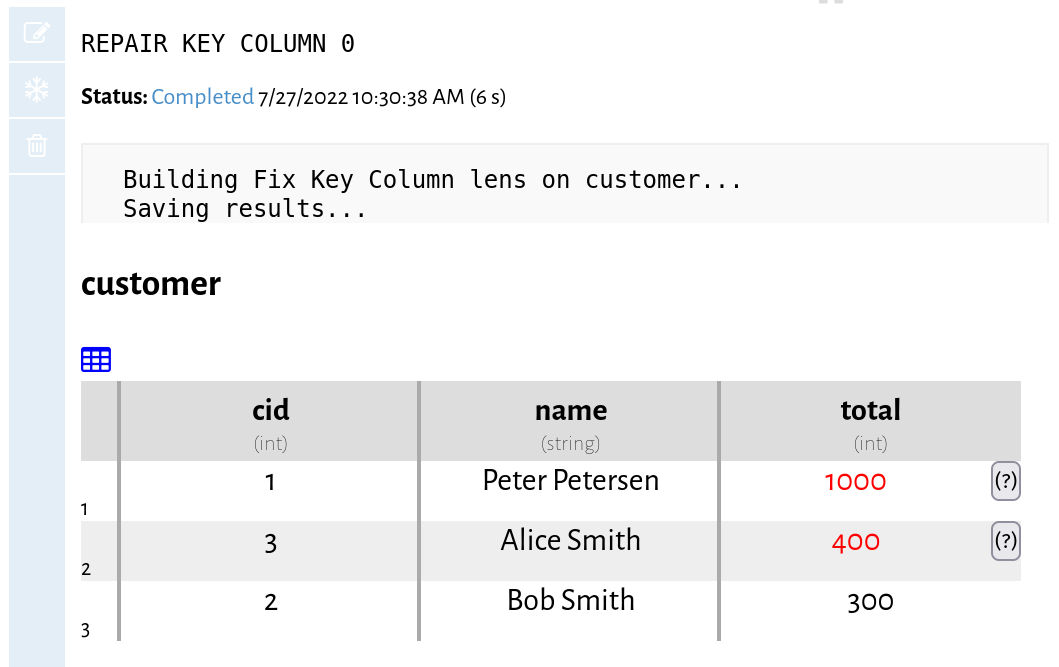
\includegraphics[width=8cm]{graphics/caveatted_data.png}
    % \begin{tabular}{c|c|c|c}
    %   \thead{cid} & \thead{name} & \thead{total} & \\       \hline
    %   1         & Peter          Petersen        & 1000 &   \\
    %   2         & Bob            Smith           & 300  & \rowcaveat  \\
    %   3         & Alice          Smith           & 400  & \rowcaveat  \\
    % \end{tabular}
    %%%%%%%%%%%%%%%%%%%%%%%%%%%%%%%%%%%%%%%%
  \caption{A UB-DB in Vizier encoding $D_1$ with possibly uncertain cells marked with caveats.}\label{fig:ub-db-encoding-d-2-with-p}
\end{wrapfigure}
%%%%%%%%%%%%%%%%%%%%%%%%%%%%%%%%%%%%%%%%
While such heuristics may be quite effective on average and are certainly superior to just randomly selecting a world, it is unavoidable that they fail for some cleaning scenarios. 
An alternative approach called consistent query answering~\cite{B11} takes a conservative stance, instead of selecting one repair, we reason about all possible repairs and only return query answers (the so-called \textit{certain answers}) that are in the query's results for every repair (i.e., are guaranteed to be in the result independent of which repair is correct). 
This approach has the advantage that only correct query answers are returned, but is computationally expensive, may exclude many very likely answers (if they are not 100\% certain), and is not closed (it is not possible to evaluate queries with certain answer semantics over the certain answers of a query).


%%%%%%%%%%%%%%%%%%%%%%%%%%%%%%%%%%%%%%%%%%%%%%%%%%%%%%%%%%%%%%%%%%%%%%%%%%%%%%%%
\subsection{Attribute- and Row-level Caveats and\\ Uncertainty-Annotated Databases}
\label{sec:attribute-row-level}
%
\begin{wrapfigure}[6]{r}[0pt]{8cm}
  \vspace*{-5mm}
  \centering
  \vspace*{-14mm}
  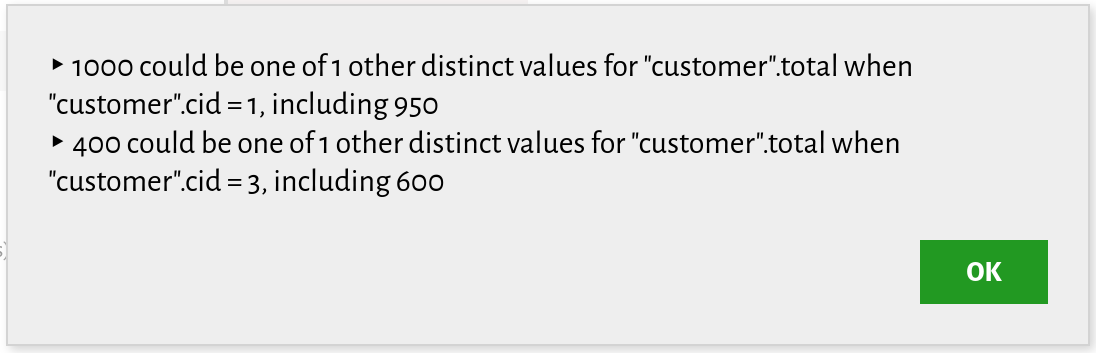
\includegraphics[width=8cm]{graphics/caveats.png}
  \caption{Caveats annotating the relation $D_1$}
\end{wrapfigure}
%


For Vizier, we developed an uncertain data model called
uncertainty-annotated databases~\cite{FH19} that annotates one
possible world (the so-called \textit{selected-guess world}) with an under-approximation  of certain answers (if we claim that a row is certain, then it is certain) that can be computed efficiently. This is encoded by annotating a subset of a dataset's rows with row-level caveats to mark them as not being certain.  The reason that we use an under-approximation is to be able to evaluate complex queries (full relational algebra including aggregation) efficiently (with PTIME data complexity and small overhead over deterministic query processing). Furthermore, attribute-level caveats are used to mark attribute values as uncertain (they may not be the same in every possible world) which is similar in nature to certain answers with nulls~\cite{L16a}.

% %%%%%%%%%%%%%%%%%%%%%%%%%%%%%%%%%%%%%%%%
% \begin{figure}[t]
%   \centering

% \begin{minipage}[b]{0.31\linewidth}
% \centering
%     \textbf{UA-DB with Selected Guess $D_1$}\\[3mm]
%     %%%%%%%%%%%%%%%%%%%%%%%%%%%%%%%%%%%%%%%
%     \begin{tabular}{c|c|c|c}
%       \thead{cid} & \thead{name} & \thead{total} & \\       \hline
%       1         & Peter          Petersen        & 1000 & \rowcaveat  \\
%       2         & Bob            Smith           & 300  & \rowcaveat  \\
%       3         & Alice          Smith           & 400  & \rowcaveat  \\
%     \end{tabular}
%     %%%%%%%%%%%%%%%%%%%%%%%%%%%%%%%%%%%%%%%%
%   \end{minipage}

%   \caption{UB-DB encoding $D_2$ with possibly uncertain rows marked with caveats (aster ix).}\label{fig:ub-db-encoding-d-2-with-p}
% \end{figure}
% %%%%%%%%%%%%%%%%%%%%%%%%%%%%%%%%%%%%%%%%

%%%%%%%%%%%%%%%%%%%%%%%%%%%%%%%%%%%%%%%%%%%%%%%%%%%%%%%%%%%%%%%%%%%%%%%%%%%%%%%%
% \subsection{Queries over Uncertainty-Annotated Databases}
% \label{sec:uncert-annot-datab}

% In~\cite{FH19} we introduced a query semantics for UA-DBs that

% %%%%%%%%%%%%%%%%%%%%%%%%%%%%%%%%%%%%%%%%%%%%%%%%%%%%%%%%%%%%%%%%%%%%%%%%%%%%%%%%
% \subsection{Implementation in Spark}
% \label{sec:implementation-spark}





%%% Local Variables:
%%% mode: latex
%%% TeX-master: "../2022_IEEE_DEB_Vizier"
%%% End:


%%%%%%%%%%%%%%%%%%%%%%%%%%%%%%%%%%%%%%%%%%%%%%%%%%%%%%%%%%%%%%%%%%%%%%%%%%%%%%%%
\section{Conclusions and Future Work}
\label{sec:conclusions}

In this paper, we have made the case for a multi-modal data science platform built on top of an incremental, data-centric workflow engine and have introduced the reader to Vizier, our system implementing this vision. 
Because each modality (notebooks, spreadsheets, the caveat view, etc\ldots) is a ``view'' interacting with the same underlying workflow and datasets, it is easy to extend the system to support new interaction paradigms in the future.  Building our system so that cells execute in isolation and only interact through dataflow makes it easy to add new cell types to the system, because we only have to worry about the interaction of the new cell type with  data artifacts. 
Thus, adding support for other interaction modalities (e.g., new programming languages) into the system is straight-forward: we implement a new cell type and an API to access Vizier artifacts from within the modality.

As demonstrated in recent preliminary work, having a scheduler that revises its schedule based on dependencies discovered at runtime and using static dataflow analysis, we can execute notebook cells in parallel and avoid re-executing cells that are guaranteed not to change during automatic refresh.
Significantly more opportunities for avoiding work exist, in particular by leveraging Vizier's standardized representation of artifacts.
For example, by representing updates to dataset artifacts as change sets, existing approaches for incremental view maintenance can reduce the runtime overhead of recomputing workflow steps, as well as the space costs of preserving multiple artifact versions. Another interesting direction for future work is to study incremental maintenance of workflow results when the definition of a workflow step changes. This is an novel variation of the traditional incremental view maintenance problem where we have to update the result based on a change to the query rather than based on a change to the data.

Similarly, standard representations of artifacts can be used to help users better understand the outputs of their workflows.
For example, numerous efforts have explored causal explanations in database query results (\cite{DBLP:conf/sigmod/KanagalLD11,DBLP:journals/pvldb/MeliouGMS11,DBLP:journals/pvldb/MeliouRS14,DBLP:journals/ftdb/GlavicMR21}, and explainability in machine learning has recently become an area of active research.
For such techniques to be truly valuable, they need to operate across artifact types. For example, what would it take to link a sudden change in predictions made by a model to the addition of a new category in source data five transformations removed from the model training step. With Vizier's uncertainty model and provenance tracking we lay the ground work to develop methods for generating explanations that span multiple steps in a workflow. 

Finally, we note that Vizier provides a ``ground-up'' approach to stitching different interaction modalities into a single workflow.
Tools implemented as views over Vizier's workflow model seamlessly interact with each other, with coarse-grained provenance, reactive cell execution, and repeatability/reproducibility.
However, these capabilities are limited to a single Vizier instance, and are of limited value to already existing tools.
An important open challenge is the design of a federated infrastructure for data analytics workflows, allowing multiple Vizier instances or unrelated tools to interoperate.


%%%%%%%%%%%%%%%%%%%%%%%%%%%%%%%%%%%%%%%%%%%%%%%%%%%%%%%%%%%%%%%%%%%%%%%%%%%%%%%%
% ACKNOWLEDGEMENTS
\mypara{Acknowledgements} This work was supported by NSF Awards ACI-1640864, IIS-1750460, IIS-1956149, and IIS-2125516. % and \ldots

%%%%%%%%%%%%%%%%%%%%%%%%%%%%%%%%%%%%%%%%%%%%%%%%%%%%%%%%%%%%%%%%%%%%%%%%%%%%%%%%
% BIBLIOGRAPHY
%\bibliographystyle{abbrv}
%\bibliography{2022_IEEE_DEB_Vizier.bib}

\documentclass[11pt]{article}

\usepackage{deauthor,times,graphicx}
\usepackage{color,colortbl}
% \usepackage[dvipsnames]{xcolor}
% \usepackage{hyperref}
\usepackage{amsmath}
\usepackage{amssymb}
\let\proof\relax
\let\endproof\relax
\usepackage{amsthm}
\usepackage{cleveref}
\usepackage{wrapfig}
\usepackage{url}
\usepackage{stmaryrd,amssymb}
\usepackage{listings}
\usepackage{algorithm}
% \usepackage[noend]{algorithmic}
\usepackage{fancybox}


%%%%%%%%%%%%%%%%%%%%%%%%%%%%%%%%%%%%%%%%
% Theorems, Definitions, Examples
%%%%%%%%%%%%%%%%%%%%%%%%%%%%%%%%%%%%%%%%
\newtheorem{theo}{Theorem}
\numberwithin{theo}{section}
\newtheorem{lem}[theo]{Lemma}
\newtheorem{propo}[theo]{Proposition}
\newtheorem{coll}[theo]{Corollary}
\newtheorem{exam}{Example}
\numberwithin{exam}{section}
\newtheorem{defi}{Definition}
\numberwithin{defi}{section}


%%%%%%%%%%%%%%%%%%%%%%%%%%%%%%%%%%%%%%%%%%%%%%%%%%%%%%%%%%%%%%%%%%%%%%%%%%%%%%%%
\usepackage{todonotes}
\newcommand{\BG}[1]{\todo[inline]{\textbf{Boris:} #1}}
\newcommand{\OK}[1]{\todo[inline]{\textbf{Oliver:} #1}}
\newcommand{\JF}[1]{\todo[inline]{\textbf{Juliana:} #1}}
\newcommand{\MB}[1]{\todo[inline]{\textbf{Mike:} #1}}

\newcommand{\jfedit}[1]{\textcolor{red} {#1}}


%%%%%%%%%%%%%%%%%%%%%%%%%%%%%%%%%%%%%%%%%%%%%%%%%%%%%%%%%%%%%%%%%%%%%%%%%%%%%%%%
% OUR SETUP
\newcommand{\mypara}[1]{\medskip\noindent\textbf{{#1}.}}

\ifdefined\thead
\else
  \newcommand{\thead}[1]{\textbf{#1}}
\fi
\newcommand{\rowcaveat}{\textbf{\textcolor{red}{$\ast$}}}
\newcommand{\pdb}{\mathcal{D}}

%%%%%%%%%%%%%%%%%%%%%%%%%%%%%%%%%%%%%%%%%%%%%%%%%%%%%%%%%%%%%%%%%%%%%%%%%%%%%%%%
% DOCUMENT
\begin{document}

%%%%%%%%%%%%%%%%%%%%%%%%%%%%%%%%%%%%%%%%%%%%%%%%%%%%%%%%%%%%%%%%%%%%%%%%%%%%%%%%
% LST DEFS

%%%%%%%%%%%%%%%%%%%%%%%%%%%%%%%%%%%%%%%%
% Colors
%%%%%%%%%%%%%%%%%%%%%%%%%%%%%%%%%%%%%%%%
\definecolor{lstpurple}{rgb}{0.5,0,0.5}
\definecolor{lstred}{rgb}{1,0,0}
\definecolor{lstreddark}{rgb}{0.7,0,0}
\definecolor{lstredl}{rgb}{0.64,0.08,0.08}
\definecolor{lstmildblue}{rgb}{0.66,0.72,0.78}
\definecolor{lstblue}{rgb}{0,0,1}
\definecolor{lstmildgreen}{rgb}{0.42,0.53,0.39}
\definecolor{lstgreen}{rgb}{0,0.5,0}
\definecolor{lstorangedark}{rgb}{0.6,0.3,0}
\definecolor{lstorange}{rgb}{0.75,0.52,0.005}
\definecolor{lstorangelight}{rgb}{0.89,0.81,0.67}
\definecolor{lstbeige}{rgb}{0.90,0.86,0.45}


% Declare bold typewriter font with Computer Modern
\DeclareFontShape{OT1}{cmtt}{bx}{n}{<5><6><7><8><9><10><10.95><12><14.4><17.28><20.74><24.88>cmttb10}{}

%%%%%%%%%% SQL + proveannce listing settings
\lstdefinestyle{psql}
{
tabsize=2,
basicstyle=\small\upshape\ttfamily,
language=SQL,
morekeywords={PROVENANCE,BASERELATION,INFLUENCE,COPY,ON,TRANSPROV,TRANSSQL,TRANSXML,CONTRIBUTION,COMPLETE,TRANSITIVE,NONTRANSITIVE,EXPLAIN,SQLTEXT,GRAPH,IS,ANNOT,THIS,XSLT,MAPPROV,cxpath,OF,TRANSACTION,SERIALIZABLE,COMMITTED,INSERT,INTO,WITH,SCN,UPDATED,PARTITION,BY,PRECEDING,FOLLOWING,CURRENT,ROW,ROWS,RANGE,GROUPING,SETS,CUBE,ROLL,UP},
extendedchars=false,
keywordstyle=\bfseries,
mathescape=true,
escapechar=@,
sensitive=true
}


%%%%%%%%%% SQL + proveannce listing settings - colorful version
\lstdefinestyle{psqlcolor}
{
tabsize=2,
basicstyle=\small\upshape\ttfamily,
language=SQL,
morekeywords={PROVENANCE,BASERELATION,INFLUENCE,COPY,ON,TRANSPROV,TRANSSQL,TRANSXML,CONTRIBUTION,COMPLETE,TRANSITIVE,NONTRANSITIVE,EXPLAIN,SQLTEXT,GRAPH,IS,ANNOT,THIS,XSLT,MAPPROV,OF,TRANSACTION,SERIALIZABLE,COMMITTED,INSERT,INTO,WITH,SCN,UPDATED},
extendedchars=false,
keywordstyle=\bfseries\color{lstpurple},
deletekeywords={count,min,max,avg,sum},
keywords=[2]{count,min,max,avg,sum,first,last,lead,lag,cxpath},
keywordstyle=[2]\color{lstblue},
stringstyle=\color{lstreddark},
commentstyle=\color{lstgreen},
mathescape=true,
escapechar=@,
sensitive=true
}


%%%%%%%%%% DATALOG style
\lstdefinestyle{datalog}
{
basicstyle=\footnotesize\upshape\ttfamily,
language=prolog
}




%%%%%%%%%% listings settings for pseudo code
\lstdefinestyle{pseudocode}
{
  tabsize=3,
  basicstyle=\small,
  language=c,
  morekeywords={if,else,foreach,case,return,in,or},
  extendedchars=true,
  mathescape=true,
  literate={:=}{{$\gets$}}1 {<=}{{$\leq$}}1 {!=}{{$\neq$}}1 {append}{{$\listconcat$}}1 {calP}{{$\cal P$}}{2},
  keywordstyle=\color{lstpurple},
  escapechar=&,
  numbers=left,
  numberstyle=\color{lstgreen}\small\bfseries,
  stepnumber=1,
  numbersep=5pt,
}

% \definecolor{pynotebookcellbg}{RGB}{247,247,247}
\definecolor{pynotebookcellbg}{gray}{0.95}

\lstdefinestyle{pynotebook}
{
  tabsize=3,
  basicstyle=\small\upshape\ttfamily,
  language=python,
  extendedchars=true,
  mathescape=true,
  morekeywords={show,read_csv,read_geojson,groupby,spatial_join,geocode,count},
  keywordstyle=\color{Blue},
  stringstyle=\itshape\color{Sepia},
  identifierstyle=\bfseries\color{OliveGreen},
  escapechar=&,
  numbers=left,
  numberstyle=\tiny\bfseries\ttfamily\color[gray]{0.7},
  stepnumber=1,
  numbersep=5pt,
  frame=single,
  frameround=tttt,
  backgroundcolor=\color{pynotebookcellbg}
}

\lstset{style=psqlcolor}

%%%%%%%%%%%%%%%%%%%%%%%%%%%%%%%%%%%%%%%%%%%%%%%%%%%%%%%%%%%%%%%%%%%%%%%%%%%%%%%%

\newcommand{\tinysection}[1]{
  \medskip \noindent \textbf{#1}.
}

%%%%%%%%%%%%%%%%%%%%%%%%%%%%%%%%%%%%%%%%%%%%%%%%%%%%%%%%%%%%%%%%%%%%%%%%%%%%%%%%
% TITLE AND AUTHORS
\title{The Right Tool for the Job: Data-Centric Workflows in Vizier}
%\title{It's a Notebook, It's a Spreadsheet, \ldots It's Vizier!}

\author{Oliver Kennedy,$^{\star}$~~Boris Glavic,$^{\diamond}$~~Juliana Freire,$^{\dagger}$~~and~~Michael Brachmann$\,^{\star}$\\
$^{\star}$~University at Buffalo, USA\\
$^{\diamond}$~Illinois Institute of Technology, USA\\
$^{\dagger}$~New York University, USA
}

\maketitle

\graphicspath{{submissions/workflow-vizier-glavic/}}

%%%%%%%%%%%%%%%%%%%%%%%%%%%%%%%%%%%%%%%%%%%%%%%%%%%%%%%%%%%%%%%%%%%%%%%%%%%%%%%%
% ABSTRACT
\begin{abstract}
  Data scientists use a wide variety of systems with a wide variety of
  user interfaces such as spreadsheets and notebooks for their data
  exploration, discovery, preprocessing, and analysis
  tasks. % For instance, spreadsheet interfaces are used for manual curation and simple types of analysis; notebook interfaces are used for data preprocessing, analysis, and visualization; and big data platforms, workflow systems, and database systems are used for more advanced querying and for deploying data analysis pipelines that were prototyped using notebooks.
  While this wide selection of tools offers data scientists the
  freedom to pick the right tool for each task, each of these tools
  has limitations (e.g., the lack of
  reproducibility % and automatic refresh of outdated results in
  of
  notebooks), % or the limited support of spreadsheets to specify batch data transformations),
  data needs to be translated between tool-specific formats, and
  common functionality such as versioning, provenance, and dealing
  with data errors often has to be implemented for each
  system. We argue that rather than alternating between task-specific
  tools, a superior approach is to build multiple user-interfaces on top
  of a single incremental workflow / dataflow platform with built-in
  support for versioning, provenance, error \& tracking, and data
  cleaning. We discuss Vizier, a notebook system that implements this
  approach, introduce the challenges that arose in building such a
  system, % , and compare the approach against state-of-the-art systems. Furthermore, we
  and highlight how our work on Vizier lead to novel research in
  uncertain data management and incremental execution of workflows.
\end{abstract}
%%%%%%%%%%%%%%%%%%%%%%%%%%%%%%%%%%%%%%%%%%%%%%%%%%%%%%%%%%%%%%%%%%%%%%%%%%%%%%%%


%%%%%%%%%%%%%%%%%%%%%%%%%%%%%%%%%%%%%%%%%%%%%%%%%%%%%%%%%%%%%%%%%%%%%%%%%%%%%%%%
\section{Introduction}
\label{sec:intro}

Federated Learning (FL) is a distributed machine learning (ML) paradigm that trains a model across a number of participating entities holding local data samples.
% , without exchanging them. 
In this work, we focus on \emph{cross-device} FL that harnesses a large number (up to hundreds of millions) of edge devices with disparate characteristics such as availability, compute, memory, or connectivity
resources~\citep{kairouz2019advances}. %that harnesses potential
% Current applications of FL are designed to scale up to client populations of hundreds of millions or even billions. 
Two challenges to the success of cross-device FL are privacy and scalability. 
FL was originally motivated for improving privacy since data points remain on client devices. 
% and only small model updates were shared to a co-ordinating server.
However, as with other forms of ML, information about training data can be extracted via membership inference or reconstruction attacks on a trained model \citep{carlini2021membership,carlini2020extracting}, or leaked through local updates~\citep{MelisSCS19,geiping2020inverting}. 
Consequently, Secure Aggregation (\SecAgg) protocols were introduced to prevent the server from directly observing individual client updates, which is a major vector for information leakage~\citep{bonavitz2019federated,huba2021papaya}. 
Additional mitigations such as  Differential Privacy (DP) may be required to offer further protection 
against attacks~\citep{dwork2006calibrating,abadi2016deep}, as discussed in Section~\ref{sec:discussion}.
% , as discussed in Section~\ref{sec:discussion}.
%As an additional layer of protection against statistical inference attacks, SecAgg is usually paired with Differential Privacy (DP) \citep{dwork2006calibrating}. To realize the full promise of FL as a privacy-enhancing technology, we need both SecAgg and Differential Privacy.

Ensuring scalability to populations of heterogeneous clients is the second challenge for FL.
% There are many aspects for FL scalability, such as ensuring that model updates can be calculated efficiently 
% by devices with various capabilities and intermittent availability~\citep{bonavitz2019federated}.
% Here, we focus on the communication bottleneck as the primary concern.
Indeed, wall-clock training times are highly correlated with increasing model and batch sizes~\citep{huba2021papaya}, even with recent efforts such as FedBuff~\citep{nguyen2021federated},
% With increasing model and batch sizes, the wall-clock training time increases accordingly~\citep{huba2021papaya}. 
% Despite efforts such as buffered asynchronous aggregation~\cite{nguyen2021federated}, 
and communication overhead between the server and clients dominates model convergence time.
% cross-device FL remains bottlenecked by communication latency between the server and the clients. 
% \karthik{should we mention this paper in a different way? Fedbuff paper doesn't explicitly call out latency as an issue, nor do we run experiments to on async fl ourselves}  \ashkan{I also think the transition can be smoother: first we focus on scalability and billions. Then we say communication is the bottleneck} 
Consequently, compression techniques were used to reduce the communication bandwidth while maintaining model accuracy.
However, a fundamental problem has been largely overlooked in the literature: in their native form, standard compression methods such as scalar quantization and pruning are not compatible with \SecAgg. 
This makes it challenging to ensure both security and communication efficiency.
% at the same time.
% the default method to provide security for client update, 
% presenting an unpleasant dichotomy between security or efficiency. 


% Second, this is the most restricted direction, since upload bandwidth remains more restricted than download. 
% In the US, fixed-line broadband speeds typically achieve a ratio of $3\times$ to $20\times$ more download bandwidth than upload
% bottlenecks remain, and so we seek to reduce the message size of clients by \textit{compression}. 
% Compression has been widely proposed in various ML scenarios, in the form of pruning (removing model parameters) and quantization (reducing fidelity of parameter representation). 
% Indeed, these techniques have been successfully used in FL settings with appreciable improvements in communication while maintaining model accuracy. 
% However, there is a fundamental problem which has been largely overlooked in the literature: in their native form, these compression methods are not compatible with SecAgg, the default method to provide security for client updates. 
% This presents an unpleasant dichotomy: we can have security or efficiency, but not both. 
%
%
% In this paper, we resolve this gap by showing how to modify FL compression techniques to make them security-friendly. We focus on compressing \emph{uplink} updates from clients to the server for two reasons. 
% First, uplink communications are subject to Secure Aggregation protocols to ensure a high security bar, while downlink updates broadcasted by the server are deemed public. 
% Second, upload bandwidth is generally more restricted than download. For instance, according to the most recent FCC report, the ratio of download to upload speeds for DSL/cable providers\footnote{Fixed-line broadband is most relevant since FL is typically restricted to using unmetered connections, usually over Wi-Fi~\citep{huba2021papaya}.} in the US ranges between 3$\times$ to 20$\times$~\citep{fcc-broadband}.
% % This requires some meticulous changes to coordinate clients to use the same global (non-private) hyperparameters, and show that this coordination does not damage model quality. 
% % For the strongest compression methods, we step outside of the SecAgg primitive and propose a new secure primitive, Secure Indexing, which enables the best compression ratios without sacrificing utility. 
% Finally, efficient and secure uplink communication brings several benefits beyond speeding up convergence: 
% lowering communication cost reduces selection bias due to undersampling clients with limited connectivity, improving fairness and inclusivity metrics. 
% It also shrinks the carbon footprint of FL, whose fraction attributable to communication can reach 95\%~\citep{qiu2021first}.
%
%In this paper, w
We address this gap by adapting compression techniques to make them compatible with \SecAgg. We focus on compressing \emph{uplink} updates from clients to the server for three reasons. 
First, uplink communication is more sensitive and so is subject to a high security bar, whereas downlink updates broadcast by the server are deemed public. 
Second, upload bandwidth is generally more restricted than download bandwidth. For instance, according to 
a recent FCC report, 
%the most recent \modif{FCC\footnote{\modif{US Federal Communications Commission.}} report}, 
the ratio of download to upload speeds for DSL and cable providers\footnote{FL is typically restricted to using unmetered connections, usually over Wi-Fi~\citep{huba2021papaya}.} in the US ranges between 3$\times$ to~20$\times$~\citep{fcc-broadband}.
% Fixed-line broadband is most relevant since
% This requires some meticulous changes to coordinate clients to use the same global (non-private) hyperparameters, and show that this coordination does not damage model quality. 
% For the strongest compression methods, we step outside of the SecAgg primitive and propose a new secure primitive, Secure Indexing, which enables the best compression ratios without sacrificing utility. 
Efficient uplink communication brings several benefits beyond speeding up convergence: 
lowering communication cost reduces selection bias due to under-sampling clients with limited connectivity, improving fairness and inclusiveness. 
It shrinks the carbon footprint of FL, the fraction of which attributable to communication can reach 95\%~\citep{qiu2021first}.
In summary, we present the following contributions: 
\begin{itemize}
    \item We highlight the fundamental mismatch between two critical components of the FL stack: \SecAgg protocols and uplink compression mechanisms.
    
    \item We formulate solutions by imposing a linearity constraint on the decompression operator, as illustrated in Figure~\ref{fig:secagg_summary} in the case of TEE-based \SecAgg.
    
    \item We adapt the popular scalar quantization and (random) pruning compression methods for compatibility with the FL stack that require no changes to the \SecAgg protocol.
    
    \item For extreme uplink compression without compromising security, we propose Secure Indexing (\SecInd), a variant of \SecAgg that supports product quantization. %and admits a secure implementation.
\end{itemize}

\begin{figure*}[t]
    \centering
    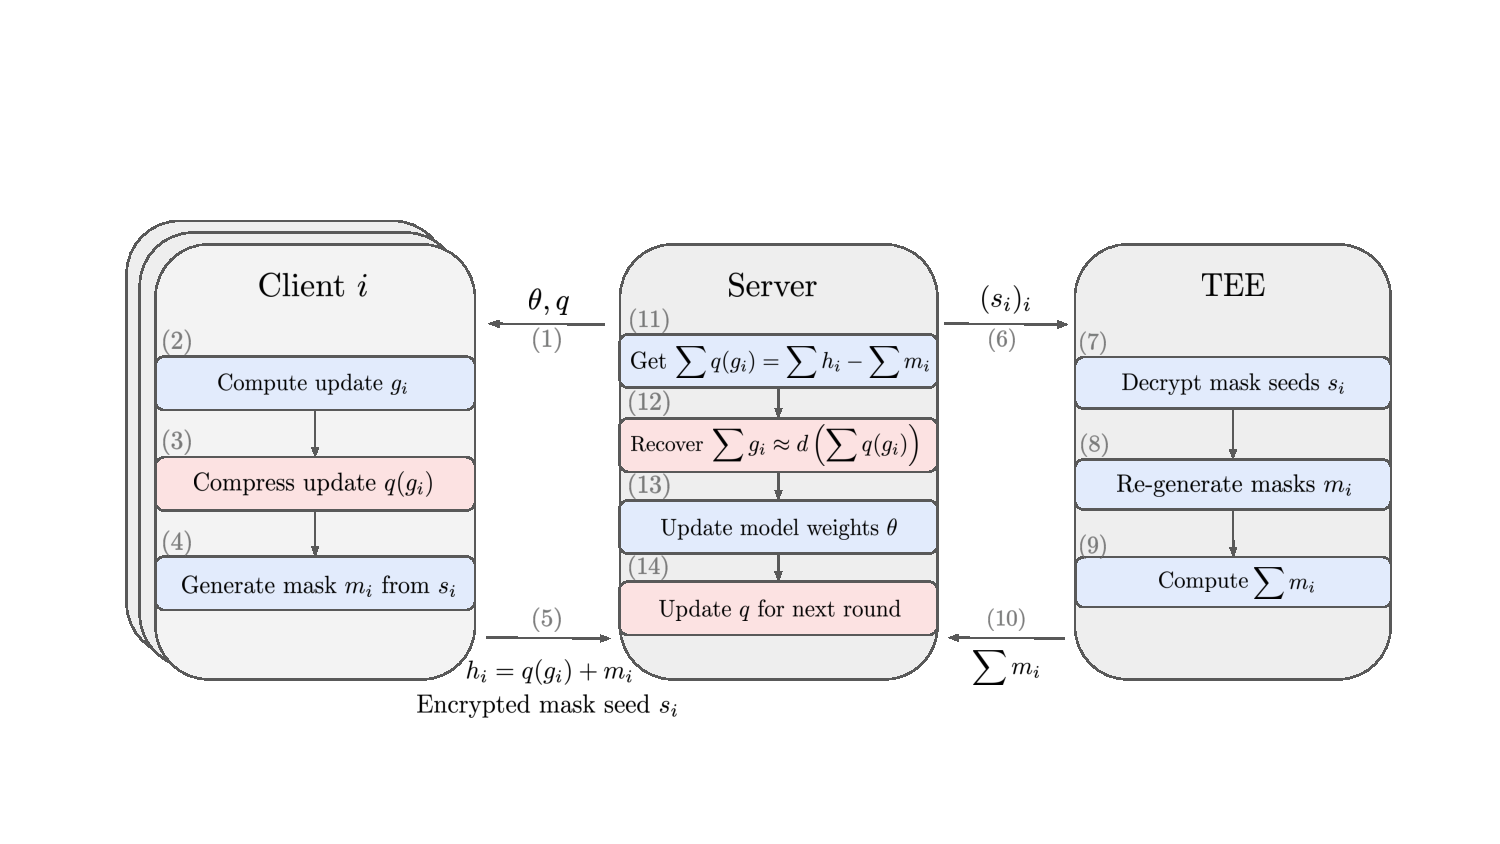
\includegraphics[width=0.8\textwidth]{figs/secagg_summary_new.pdf}
    %\vspace{-5mm}
    \caption{\label{fig:secagg_summary}
    Summary of the proposed approach for one FL round, where we omit the round dependency and \modif{Differential Privacy (DP)} for clarity. Blue boxes denote standard steps and red boxes denote additional steps for uplink compression. Client $i$ computes local model update $g_i$, compresses it with the compression operator $q$, and encrypts it by adding a random mask $m_i$ in the compressed domain, hence reducing the uplink bandwidth (steps 2--4). The server recovers the aggregate in the compressed domain by leveraging any \SecAgg protocol \modif{(steps 7--13, with a TEE-based \SecAgg, see Section~\ref{subsec:secagg})}. Since the decompression operator $d$ is linear, the server can convert the aggregate back to the non-compressed domain, up to compression error (step 12). As with the model weights $\theta$, the compression operator $q$ are also periodically updated and broadcast by the server (step 14). 
    In Section~\ref{sec:method}, we apply the proposed method to scalar quantization and pruning without impacting \SecAgg and propose Secure Indexing, a variant of \SecAgg for extreme uplink compression with product quantization. See Section~\ref{subsec:secagg} for details about \SecAgg and Section~\ref{sec:discussion} for a discussion on~DP.
    }
    \vspace{-3mm}
\end{figure*}



% Our focus in this paper is on 

%Second, scaling cross-device (synchronous) FL to millions of clients with various capabilities and intermittent availability \citep{bonavitz2019federated} suffers from diminishing returns: the wall-clock training time plateaus as the number of clients keeps increasing~\citep{huba2021papaya}. Even though this challenge can be addressed by leveraging the buffered asynchronous aggregation technique proposed by \cite{nguyen2021federated}, compatible with DP and SecAgg, the asynchronous protocol remains bottlenecked by communication latency between the server and the clients.


%Considering the above privacy and scalability goals, we focus on enabling efficient FL communications while keeping a high privacy bar. In addition to the primary objective of speeding up convergence, reducing communication costs brings other significant benefits. Lowering communication requirements addresses selection bias due to undersampling clients with limited connectivity, improving fairness and inclusivity metrics. Better communication efficiency shrinks the carbon footprint of FL, whose fraction attributable to communication can reach 95\%~\citep{qiu2021first}. %Finally, training larger model in FL would be a possibility, when the communication cost is reduced, because local memory or compute requirements can be addressed by modifying the local training loop, for instance with gradient checkpointing \citep{chen2016training}. However, some form of compression would be required to enable efficient communication.


%First, compressing model updates from the client to the server presents several challenges due to compatibility with SecAgg and is an area suitable for further research. 
%Second, upload bandwidth is generally more restricted than download. For instance, according to the most recent FCC report, the ratio of download to upload speeds for DSL/cable providers in the US ranges between 3$\times$ to 20$\times$~\citep{fcc-broadband}. We consider broadband speeds here because devices participate in the FL training while connected to fixed broadband, usually through Wi-Fi~\citep{huba2021papaya}.




% Hence, FL provides the ability to leverage data from massive client populations while ensuring the security and privacy of the client data.
% Go further: compatibility with DP / compression as a mitigation techniques of attacks
% Model and gradient compression intrinsically different.
%  Why not having the secure enclave perform the aggregation?
% \section{Requirements for a Multi-modal Data Science Platform}
\label{sec:requ-holist-data}

In this section we outline the requirements of a multi-modal data science platform and then introduce Vizier as a solution fulfilling these requirements. We start by discussing existing modalities that are widely used to interact with data in data science and their advantages and disadvantages. Converging on a set of modalities we deem to be essential, we then cover several cross-cutting concerns such as reproducibility and dealing with errors that are important no matter what modality is used to interact with data.

%%%%%%%%%%%%%%%%%%%%%%%%%%%%%%%%%%%%%%%%%%%%%%%%%%%%%%%%%%%%%%%%%%%%%%%%%%%%%%%%
\subsection{Modalities for Interacting with Data}
\label{sec:modal-inter-with}

Data scientists often employ several tools during the life-cycle of building a data pipelines. During data discovery, search engines (e.g., open data repositories) and dataset discovery tools (e.g., metadata management tools for data lakes) are used to identify data internal to an organization, data available for purchase, or openly available data that could be used to fulfill the goal the data scientist has in mind. The next step is typically to profile the data and understand its semantics and fitness for the task at hand. At this stage, data visualization is used, either in the form of specialized visualization systems or by employing visualization libraries written in, e.g., Python. This is often done from within notebook environments like Jupyter which can show visualizations inline with the users code. Afterwards, data is curated and integrated. Spreadsheets are often used for manual inspection of smaller datasets, repair of one-off errors, and to calculate basic statistics. Task-specific data cleaning systems or libraries written in a general purpose programming language are employed to (partially) automate this process. The cleaned and integrated data is then used in data analysis (e.g., building and evaluating machine learning models, running analytical queries, \ldots) and the final results of the analysis are visualized. Building a data pipeline is often an iterative process where the user revisits previous steps in the pipeline to deal with errors and to refine the processing.

%%%%%%%%%%%%%%%%%%%%%%%%%%%%%%%%%%%%%%%%%%%%%%%%%%%%%%%%%%%%%%%%%%%%%%%%%%%%%%%%
\subsubsection{Notebooks for Interactive Pipeline Development with Immediate Feedback}
\label{sec:noteb-inter-pipel}
%
Notebook systems like Jupyter and Apache Zeppelin to name just a few have become the quasi-standard for developing data science pipelines. One major advantage of notebooks is their highly interactive nature: users can run pieces of code and immediately observe their results. This makes it easy to debug steps in the pipeline and aids iterative development of pipelines. The outputs recorded in a notebook serve as a documentation of the data preparation and analysis process. Furthermore, most notebook system allow support documentation (typically written in a markup language such as markdown) to be interleaved with code. Even notebook interfaces have become prevalent, most existing implementations are suffer from poor reproducibility, do not support iterative development well, and are not suited well for large and complex pipelines. A recent study~\cite{PM19} on Jupyter notebooks collected from github observed that only 4\% of these notebooks are reproducibly in the sense that they can be rerun without errors and produce the same result as recorded in the notebook. We have argued in \cite{BS20, DG22} that these shortcomings are not inherent to the notebook model, but rather are the result of the architecture of notebook systems which use a long running kernel (e.g., a Python interpreter) and when the user runs a cell in a notebook send the cell's code to the kernel for execution. The kernels state, however, is hidden from the user and except for cell outputs is not encoded in the notebook itself. This leads to unreproducible behavior where the results recorded in the notebook no longer agree with a serial (top-down) execution of the notebook's cells. Furthermore, this can lead to stale results, if the user forgets to rerun cells whose code does dependent on the code in a cell that has been changed. Given the many benefits of and broad use of notebooks, support for a notebook interface is a must for any data science platform. We argue that by providing a notebook interface on top of a specialized workflow engine we can avoid the pitfalls of notebook systems which are thin wrappers around a kernel (Python interpreter). Specifically, we want a solution that supports a notebook interface (\textbf{requirement (N)} which fulfills the following conditions:
\begin{itemize}
\item \textbf{(N1) Serial Execution Semantics:} At any point in time, the results for the cells of the notebook agree with the results produced by a serial execution of the notebook.
\item \textbf{(N2) No Stale Outputs:} The outputs of each cell in the notebook should correctly reflect the current version of the notebook's code.
\item \textbf{(N3) Reproducibility:} The execution of a pipeline (notebook) does not depend on any hidden state. That is, as long as the code in the notebook is deterministic, rerunning a pipeline produces the same output as the original execution.
\end{itemize}

Note that any system that guarantees serial execution of notebooks as defined above, automatically guarantees that there are no stale outputs and that the execution of a notebook is reproducible.


%%%%%%%%%%%%%%%%%%%%%%%%%%%%%%%%%%%%%%%%%%%%%%%%%%%%%%%%%%%%%%%%%%%%%%%%%%%%%%%%
\subsubsection{Spreadsheets for Manual Curation and Exploration}
\label{sec:spre-manu-curat}
%
While notebooks are suited well for programmatic transformation and exploration of data, spreadsheet interfaces enable manual exploration and one-off transformations and fixes~\cite{FG16}. For instance, a user may search for and correct a few mistyped attributes values through a spreadsheet interface. Spreadsheets are also suited well for testing simple data transformations on a few rows using formulas and then once the transformation is satisfactory apply the transformation to a large number of rows by applying the same formula to many rows. Many spreadsheet systems have support for tracking changes made to the spreadsheet, but lack mechanisms to navigate the version history of a spreadsheet and to create branches, e.g., to try out a crazy idea without breaking a deployed version of a data science pipeline. As observed elsewhere~\cite{bendre-19-fhs}, spreadsheet systems do not typically scale to large datasets. While it is anyways infeasible to manually clean and curate large datasets, developing manual fixes on a sample / subset of a large dataset and then deploying the fixes to the dataset can be quite effective. Most spreadsheet systems use a data model that is incompatible with other structured data models such as the relational data model or data frames (which are essentially relations with row indexes) in that (i) columns do not have to be declared but are used by inserting a value into one cell of a column, (ii) the values of a column do not need to belong to a single datatype (e.g., some cells in a column may store strings while others are integers), and (iii) some operations  change the row and column positions rather than their content (e.g., inserting a row, changes the positions of all following rows). To support spreadsheets as a modality (\textbf{requirement (S)}, data science platforms should:
\begin{itemize}
\item \textbf{(S1) Translating between Relations and Spreadsheets:} It should be possible to manipulate standard relations through a spreadsheet view as well as process spreadsheets in other modalities.
\item \textbf{(S2) Supporting Spreadsheet Operations over Relations:} It should be possible to apply spreadsheet operations such as inserting / deleting rows / columns.
\item \textbf{(S3) Scalability:} It should be possible access large datasets through a spreadsheet interface.
\end{itemize}

%%%%%%%%%%%%%%%%%%%%%%%%%%%%%%%%%%%%%%%%%%%%%%%%%%%%%%%%%%%%%%%%%%%%%%%%%%%%%%%%
\subsubsection{Profiling and Interactive Visualizations}
\label{sec:inter-visu}
%
Data profiling and visualization are important tools for data scientists to explore data, understands its semantics, and identify problems with the data.
Data science platforms should support visualizations (\textbf{requirement (V)}). For example, a typical task in the initial data exploration phase of constructing a pipeline is to analyze and visualize the data distributions of columns in a dataset, e.g., by computing histograms for individual columns or by calculating the number of null values per column. Another common approach is to visualize correlations between columns. Both the spreadsheet and notebook modalities discussed so far, do support creation of plots and other data visualizations. Visualization recommendation~\cite{lee-21-l, hu-19-v} guide the user in exploring visualizations that help them to understand their data. A data science platform should support out-of-the-box visualizations  for common tasks (\textbf{requirement (V1)}, e.g., accessing data distributions as histograms as well as provide access to more general visualization tools (\textbf{requirement (V2)} to enable creation of custom visualization of, e.g., analysis results.

%%%%%%%%%%%%%%%%%%%%%%%%%%%%%%%%%%%%%%%%%%%%%%%%%%%%%%%%%%%%%%%%%%%%%%%%%%%%%%%%
\subsubsection{Semi-automated Data Cleaning, Curation, and Integration}
\label{sec:semi-automated-data}
%
As has been observed repeatedly in the past~\cite{nyt:wrangling}, data scientists spend the majority of their time in data discovery, preparation, and curation. Data cleaning, integration, and curation are complex tasks that are time consuming and error-prone. While full automation of these tasks is typically not an option, a plethora of semi-automated tools (e.g., constraint-based data cleaning~\cite{ilyas-15-tcrd}, schema matching~\cite{RB01}, and data integration~\cite{HR06}) which rely on heuristics and often involve the user in curation decisions have been proposed and exist in the form of stand-alone tools and libraries available for languages such as Python. Data science platforms should enable users to use such tools and algorithms in their data science pipelines (\textbf{requirement (C)}. Most approaches for automating data wrangling rely on heuristics to clean data. This is due to the fact that typically insufficient information is available to determine what the correct repair for a dataset is. For instance, when repairing a primary key constraint by tuple deletion~\cite{ilyas-15-tcrd}, one has to retain at most one tuple from each group of tuples with the same primary key value, however, we typically lack information to decide which tuple is the correct one to keep. Thus, data repair algorithms instead use heuristics such as preferring tuples with values that are common in the dataset or optimizing a global metric~\cite{RC17}. Data science platforms should track changes made based on heuristics and how they affect downstream operations as well as provide the user with an overview of what other choices did exist and how different choices would have affected the user's analysis results (\textbf{requirement (U)}):
\begin{itemize}
\item \textbf{(C) (Semi-)automated Data Curation and Integration:} Data science platforms should empower users to access (automated) data curation, cleaning, and integration techniques.
\item \textbf{(U) Tracking the Impact of Uncertain Choices:}  The impact of heuristic choices should be tracked through the operations in a data pipeline to aide the user in understanding how these choices have affected their analysis results and how the results would be affected if another alternative would have been chosen during data cleaning.
\end{itemize}

In summary, all modalities we have discussed so far have in common that they provide ways for the user to interact with data by applying transformations that create new data artifacts or update existing data artifacts and by viewing artifacts through user interfaces. For instance, plotting a histogram of the value distribution of an attribute in a csv file involves several transformations: (i) load the CSV file into a suitable in-memory data structure (e.g., a Pandas dataframe); (ii) aggregate the data to create a histogram; (iii) transform the histogram into a plot. We argue that it is feasible to build multiple modalities as ``views'' on top of a single dataflow platform. This approach has the advantage that the user does not have to to manually transform data between different formats expected by systems implementing the different modalities. Even more important, critical orthogonal functionality  such as versioning (that we will discuss next) has to only be implemented once.

%%%%%%%%%%%%%%%%%%%%%%%%%%%%%%%%%%%%%%%%%%%%%%%%%%%%%%%%%%%%%%%%%%%%%%%%%%%%%%%%
\subsection{Cross-cutting Concerns}
\label{sec:cross-cutt-conc}

Independent of which modality is used to interact with the data, there are important cross-cutting concerns such as reproducibility, supporting the user in iterative development of their data pipelines, dealing with data errors and uncertainty, and how to document data which need to be addressed. Some of the issues with implementing these cross-cutting functionality for specific modalities was already discussing in \Cref{sec:modal-inter-with}, but here we

\begin{itemize}
\item \textbf{(R) Reproducibility and Versioning:} Developing a data science pipeline typically requires several rounds of iterative development and refinement and may involve more than one developer. Keeping track of versions of the pipeline (and the associated results) in a version control manner is critical for aiding users in their development process (e.g., roll back to a past working version of the pipeline or test an experimental idea in a separate branch). However, we argue that unlike in version control systems where the user decides which versions of their code are persisted, for data science platforms it is beneficial if by default all past versions are retained (\textbf{requirement (R1)}). That is there should be no difference between the state kept for supporting undo as well as state kept for versioning. Furthermore, for reproducibility, unless the user's code contains non-deterministic operations, repeated executions of a pipeline should return the same result. Since we want to support interactive modalities like spreadsheets, modifications made through such modalities (e.g., manual edits of cell values or inserting and deleting rows in a spreadsheet) have to be translated into steps in the pipeline (\textbf{requirement (R2)}).
\item \textbf{(I) Supporting Iterative Refinement of Pipelines:} Data pipelines are typically constructed in an iterative fashion by adding additional steps and revisiting prior steps in the pipeline. For example, if an analysis returns unexpected results, the user may backtrack and modify steps in the pipeline which clean the data that is used in the analysis. A data science platform should support users in this process by (i) providing an overview of the structure of the pipeline to help the user to navigate between different parts of the pipeline (\textbf{requirement (O)}), (ii) by providing coarse-grained provenance to help the user identify which steps affected the data used by a pipeline step (\textbf{requirement (P)}), and (iii) ensure that outputs of pipeline steps are always up to date when upstream steps are modified. Note that the last requirement is the ``no stale outputs'' requirement (\textbf{requirement (N2)}) we have already discussed in \Cref{sec:noteb-inter-pipel}.
\item \textbf{(D) Documenting Data and Operations:} One advantage of notebook style interfaces is that they allow code and data to be documented using a markup language. For instance, a user may use this feature to document some insights into the semantics of their data or to explain why they selected a particular cleaning or learning technique. However, documentation in notebooks is associated with steps in the pipeline (cells in the notebook) rather than with pieces of data. While this type of documentation should be support (\textbf{requirement (D1)}), data documentation serves a wide range of purposes such as documenting data semantics (e.g., the year for a column storing dates as a month and day of the month), encoding information of how data was collected and processed, and recording information about issues with the data (e.g., a heart rate measurement is outside of the physically possible range). In \cite{kumari:2021:cidr:datasense} we argued that documentation pertaining to data is mission critical should be associated with the data (\textbf{requirement (D2)}) and should persist through operations (\textbf{requirement (D3)}). For instance, if the user annotated some values in a dataset with a note explaining that these values are suspicious, then aggregated summaries derived from the data should also be associated with these notes.
\item \textbf{(E) Dealing with Errors and Uncertainty:} Uncertainty and errors are prevalent in many application domains due to sensor, outliers~\cite{HA04}, and data entry errors, heuristics applied during data curation, integration~\cite{AS10, FK11b}, and cleaning~\cite{YM15, BS10a}, and misinterpretation of data semantics. Data science platforms should help users in identifying errors, should provide access to semi-automated (heuristic) methods for cleaning and curating data such as the data repair techniques~\cite{B19, ilyas-15-tcrd}. Furthermore, the platform should help the user to determine how choices made during cleaning (whether by a human or an algorithm) affect the results of analyzing the data.
\end{itemize}

In this section we have outlined a set of requirements, both to support specific modalities of interacting with data as well as general requirements that any system for building data science pipelines should support.


%%% Local Variables:
%%% mode: latex
%%% TeX-master: "../2022_IEEE_DEB_Vizier"
%%% End:

%!TEX root=../2022_IEEE_DEB_Vizier.tex

% %%%%%%%%%%%%%%%%%%%%%%%%%%%%%%%%%%%%%%%%
% \begin{figure}[t]
%   \centering
%   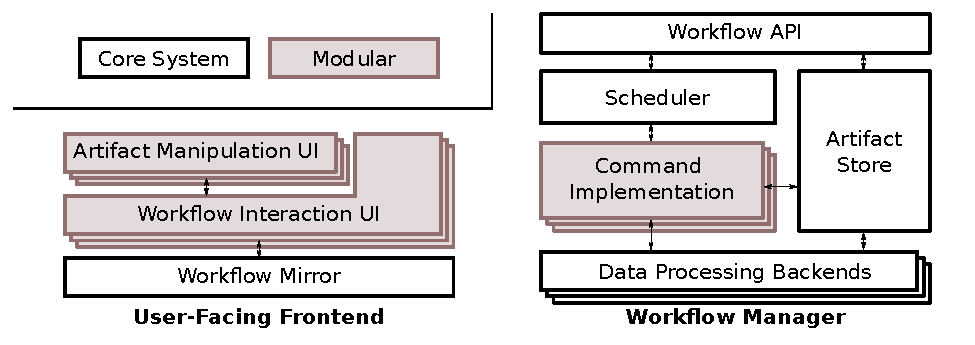
\includegraphics[width=0.7\textwidth]{graphics/systemarch}\\[-5mm]
%   \caption{Vizier's architecture, comprised of a user-facing frontend component and a backend component.}\label{fig:vizier-architecture}
% \end{figure}
% %%%%%%%%%%%%%%%%%%%%%%%%%%%%%%%%%%%%%%%%

%%%%%%%%%%%%%%%%%%%%%%%%%%%%%%%%%%%%%%%%%%%%%%%%%%%%%%%%%%%%%%%%%%%%%%%%%%%%%%%%
\pagebreak[4]
\subsection{Solution Overview}
\label{sec:solution-overview}

%%%%%%%%%%%%%%%%%%%%%%%%%%%%%%%%%%%%%%%%
\begin{wrapfigure}[12]{r}[0pt]{12cm}
  \centering
  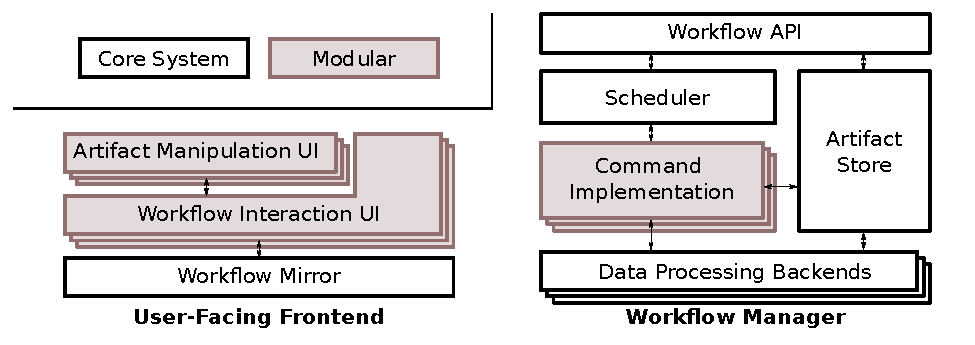
\includegraphics[width=0.7\textwidth]{graphics/systemarch}\\[-5mm]
  \caption{Vizier's architecture, comprised of a user-facing frontend component and a backend component.}\label{fig:vizier-architecture}
\end{wrapfigure}
%%%%%%%%%%%%%%%%%%%%%%%%%%%%%%%%%%%%%%%%
An overview of Vizier's architecture is shown in \Cref{fig:vizier-architecture}.
Addressing requirement \textbf{W1}, the central abstraction in Vizier is a workflow: a linear sequence of steps. % taken by the user in pursuit of a specific objective.
Unlike classical workflow systems, Vizier does not require users to explicitly declare information flow between steps.
Rather Vizier borrows the model employed in popular computational notebooks like Jupyter, where inter-cell communication occurs through a global state (artifacts) passed sequentially through steps.
Following notebook conventions, we refer to these steps as \emph{cells}, and the global state as a \emph{scope}, a map from artifact name to the version of the artifact valid at this point in the workflow. Vizier stores artifacts in common formats through a versioned \textbf{Artifact Store} (\Cref{sec:data-artifacts}), addressing requirement \textbf{A2}.
In \Cref{sec:vizier-workflows}, we formalize Vizier's workflow model, and show how we satisfy requirement \textbf{W3} by instrumenting how each cell interacts with the scope, allowing us to determine what artifact versions are valid.

Vizier's workflow semantics, paired with the versioned artifact store and workflow versioning (\Cref{sec:vizier-history}) addresses requirement \textbf{W2}. % as notebooks have a natural concept of logical order (the order of cells in the notebook) that can be adjusted over time.
% Adding workflow versioning  is sufficient to fully address the requirement.
In contrast, classical notebooks like Jupyter or Zeppelin rely on the global state of an interpreter for inter-cell communication.
Reverting this state to an earlier revision is challenging~\cite{zelnicki:2017:nodebook}, limiting their ability to satisfy requirement \textbf{W3}.
Vizier instead relies on its versioning system, allowing its \textbf{Scheduler} to automatically detect and re-evaluate stale cells (\Cref{sec:vizier-scheduler}).
To address requirement \textbf{A3}, we designed a light-weight uncertain data model that is implemented in Vizier in the form of \textit{caveats}, annotations on data that indicate uncertain values and rows  (\Cref{sec:data-docum-error}).

Addressing requirement \textbf{A1} requires modularity in both Vizier's front- and back-end components.
First, the user's interactions with a workflow and artifacts, whether through a scripting language, graphical interaction, or any other modality, need to be captured for replay (simultaneously addressing requirement \textbf{A4}). In Vizier this is achieved by requiring that every update to an artifact made through a particular modality has to be reflected as an operation in the workflow, i.e., a data update is translated into a workflow update.
Vizier manages a collection of \textbf{Command Implementations} that implement the logic behind these artifact transformations (\Cref{sec:multimodality}).
To streamline the implementation of commands, Vizier's data formats and transformations are built over standard \textbf{Data Processing Backends} like Apache Spark.
% For example, Vizier supports fine-grained provenance over datasets by encoding them as Spark data frames.

The frontend is implemented over a \textbf{Workflow Mirror} that uses websockets to reflect a live view of the workflow the user is editing.
Vizier automatically derives a default \textbf{Artifact Manipulation User Interface} for its notebook interface from each command's parameter schemas. This interface suffices for many templated commands, but the frontend can be further extended to provide a more customized experience, for example for Spreadsheet-style direct manipulation of data (\Cref{sec:spreadsheets}).
As illustrated in \Cref{fig:screenshot}, the frontend displays three \textbf{Workflow Interaction User Interfaces} by default: (i) A direct display of the workflow as a notebook, (ii) a table of contents summary of the notebook, including highlighting from documentation, and (iii) a list of artifacts derived by the notebook.
Several of these components, including the notebook and the artifact list provide access to direct manipulation interfaces.
Additional views currently implemented in Vizier include: (iv) A caveat view (\Cref{sec:data-docum-error}) that shows and tracks potential errors in the workflow and data, (v) a history view that shows the evolution of the workflow over time, and (vi) a data provenance subway diagram view.

%%%%%%%%%%%%%%%%%%%%%%%%%%%%%%%%%%%%%%%%%%%%%%%%%%%%%%%%%%%%%%%%%%%%%%%%%%%%%%%%
\begin{figure}
  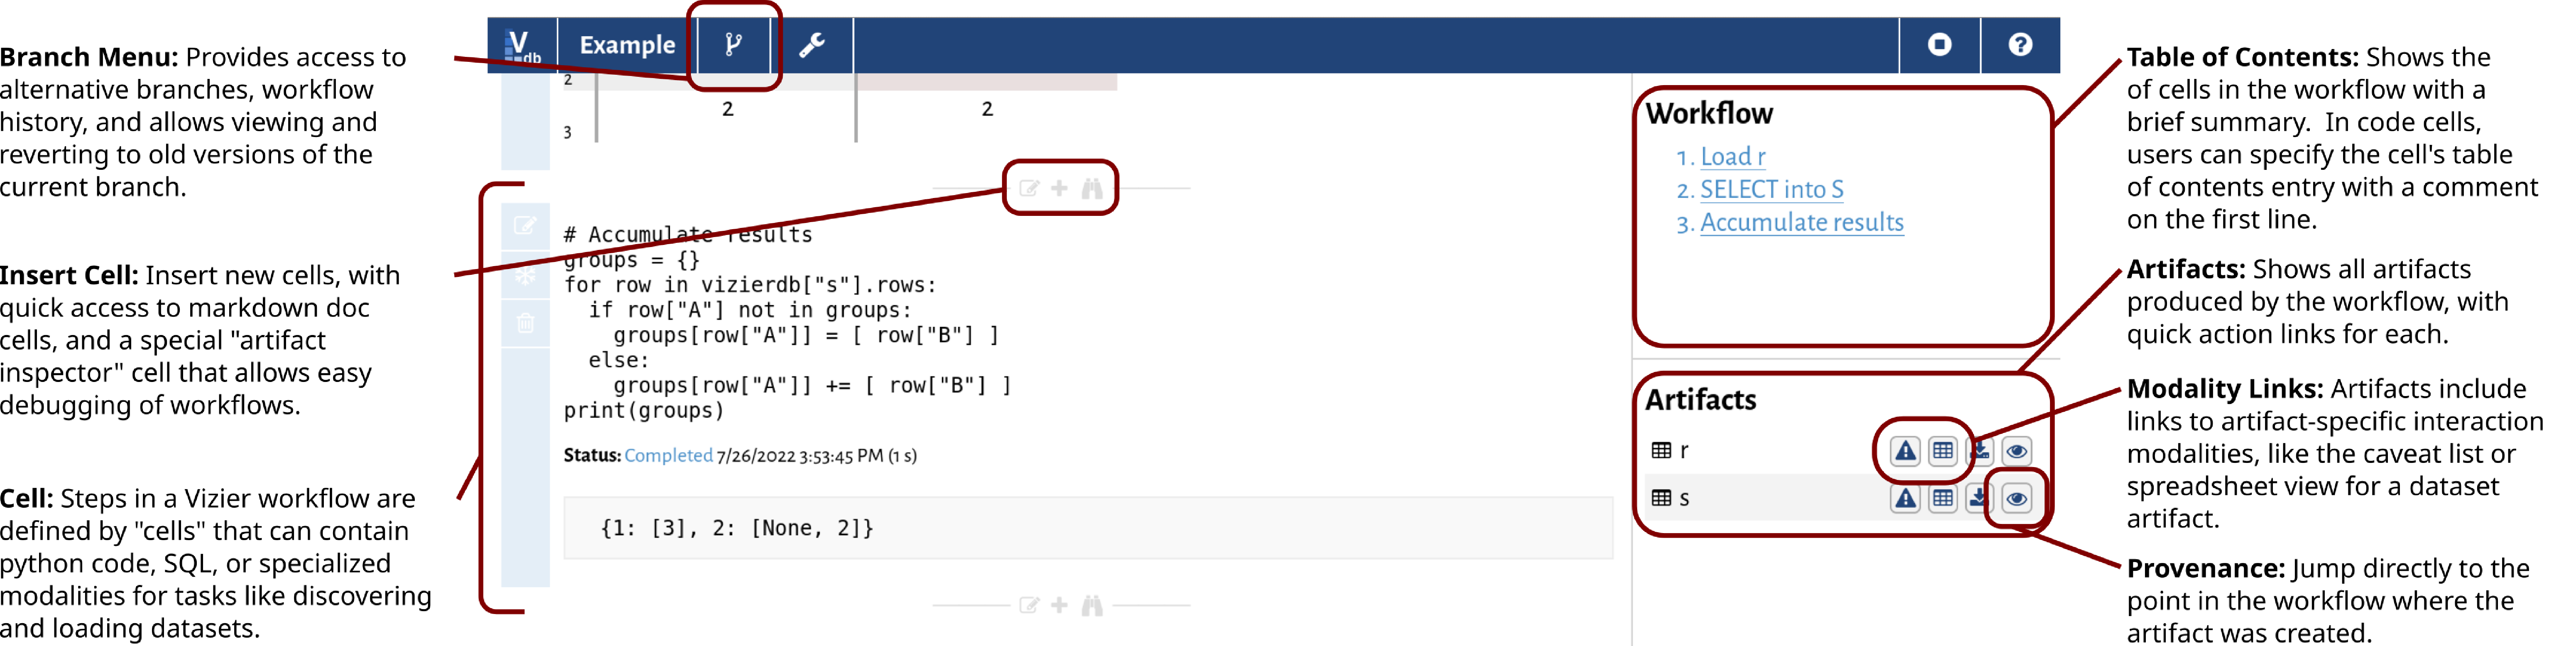
\includegraphics[width=\textwidth]{graphics/screenshot.pdf} 
  \caption{The Vizier User Interface}
  \label{fig:screenshot}
\end{figure}
%%%%%%%%%%%%%%%%%%%%%%%%%%%%%%%%%%%%%%%%%%%%%%%%%%%%%%%%%%%%%%%%%%%%%%%%%%%%%%%%

%%% Local Variables:
%%% mode: latex
%%% TeX-master: "../2022_IEEE_DEB_Vizier"
%%% End:

%!TEX root=../2022_IEEE_DEB_Vizier.tex
%%%%%%%%%%%%%%%%%%%%%%%%%%%%%%%%%%%%%%%%%%%%%%%%%%%%%%%%%%%%%%%%%%%%%%%%%%%%%%%%
\section{Versioned Data Artifact Store}
\label{sec:data-artifacts}

Steps in Vizier workflows create, read, and update \textit{``data artifacts''} or artifacts for short.
To maximize interoperability between cells, Vizier establishes standards for how these artifacts are serialized, which we now discuss. Versions of artifacts are immutable. 
An update to an artifact creates a new object representing the updated artifact. Immutability greatly simplifies handling of state in Vizier and enables us to share artifact versions across multiple revisions of a workflow.

\mypara{Dataset Artifacts}
Tabular data is represented by Vizier as a Spark dataframe~\cite{AX15}, a logical encoding of how a dataset is derived from source data.
The choice to store datasets through a logical representation (specifying the computation instead of its result) is driven largely by the need for managing annotations (requirement \textbf{A3} which is implemented by rewriting the computation to handle annotations), but also results in lower space consumption.
% Because data frames are not serializable, Vizier instead stores dataframe constructors: standardized logic for instantiating a data frame, e.g. by transforming or applying other artifacts.

% Vizier's dataframe constructors are a close analog of SparkML's \texttt{Pipeline}s, which provide a serializable representation of data frame transformation logic.
% Although Vizier provides a pipeline data frame constructor, Pipelines are strictly a representation of transformations, normally requiring glue code to apply the pipeline to an independently loaded dataset;
% Constructors completely capture the logic needed to instantiate a dataframe.

\mypara{Parameter Artifacts}
A parameter artifact can be any primitive value of any data type supported by Apache Spark; We note that this includes simple nested collections like Arrays and Maps.
This type of artifact provides a way to parameterize scripts and other system components, particularly for non-technical users.
% Vizier provides a ``Set Parameter'' command that allows users to specify parameters;
and parameter artifacts are used to pass simple data (e.g., simple constants in Python) between cells.

In addition to these two artifact types, Vizier also supports plots (stored in the vegalite~ \cite{DBLP:journals/tvcg/SatyanarayanMWH17} format), blobs and uninterpreted files, and language-specific constructs, e.g., Python function definitions. For lack of space, we do not further  discuss these other artifact types.

% \mypara{Chart Artifacts}
% Although Vizier provides means for plot generation (e.g., Bokeh, Matplotlib) through messages emitted by a cell, a standardized vegalite~\cite{DBLP:journals/tvcg/SatyanarayanMWH17} artifact format allows multiple cells to collaboratively edit a plot.
% For example, a ``Chart'' command makes it easy for users to quickly visualize a dataset, and then a Spark or Python cell can refine the resulting visualization by tweaking labels, adding markers, or adjusting colors.

% \mypara{Blob and File Artifacts}
% As a fallback to other data formats, Vizier allows cells to export state through a simple blob format.
% For example, Python falls back to encoding global state in `pickle' format, which is stored as a simple blob.
% The blob store is encoded as an in-memory array; If the artifact is large enough to warrant disk IO (e.g., a large model), requires a directory structure (e.g., parquet files), or is otherwise tied to the filesystem, Vizier provide a file artifact format.
% File artifacts are stored in a unique location tied to the artifact identifier.

% \mypara{Function Artifacts}
% Symbols representing language-specific constructs like functions, classes, and imported modules are encoded as raw code.
% Each artifact stores condains code that defines a single symbol under a specific name.
% At time of writing, support for function artifacts requires explicit cross-platform implementation support, although efforts are under way to provide a standardized cross-language interface.




%%% Local Variables:
%%% mode: latex
%%% TeX-master: "../2022_IEEE_DEB_Vizier"
%%% End:

% %!TEX root=../2022_IEEE_DEB_Vizier.tex
\section{Microkernel Notebooks}
As we outline above, a typical computational notebook relies on a kernel, a long-lived interpreter for a scripting language for a scripting language like python that retains the notebook's intermediate state.
When a cell is executed by the user, its contents are evaluated by the long running interpreter; the interpreter's state changes, and any output produced by the cell (e.g., console logs, charts, or maps) is displayed alongside the cell.
This behavior is independent of the order in which the cell appears in the notebook: The user may return to an earlier cell and modify it, but this cell is simply run against the current state of the interpreter.

Although this design allows users to revise cells in the notebook without being forced to re-run all of the notebooks code from scratch, it does pose several problems.
Most notably that it forces users to reason about the internal state of the kernel, for example by manually adopting a single static assignment variable allocation pattern.
Second, it also requires users to manually keep track of how different notebook cells relate to one-another; When a cell is modified, other cells that depend on it may also need revision.
Finally, in this design, persistence (e.g., of the results of a slow-running computation) must be managed entirely by the user.
Moreover, it is up to the user to manually manage this state to ensure consistent versioning, and portability.

One class of systems including Vizier~\cite{BS20,BB19} and Nodebook address these challenges by checkpointing global notebook state in between cell executions and restoring it when a cell is re-executed.
Thus, the cell is always evaluated on the state version emitted by the preceding cell, and changes to the state can be identified so that subsequent cells that depend on modified outputs can be re-evaluated.
This model 


\begin{itemize}
	\item Standard API for interacting with notebook state facilitates multi-modality
	\begin{itemize}
		\item No $N^2$ problem like for jupyter kernels
		\item Not just notebooks
	\end{itemize}
	\item Typed API allows fine-grained provenance
	\begin{itemize}
		\item Reproducibility
		\item Automatic refresh
		\item No hidden (mystical) dependencies
	\end{itemize}
	\item Challenges:
	\begin{itemize}
		\item Communicating state between kernels
		\item 2-dimensional version model (cell-order vs historical-order <- better name for this exists)
		\item Input/output changes in history vs Operation changes in history
		\begin{itemize}
			\item Vizier: Module vs Cell vs Result
			\item The Vizier execution state-model
		\end{itemize}
		\item Scheduling / Deciding state
	\end{itemize}
\end{itemize}

%%% Local Variables:
%%% mode: latex
%%% TeX-master: "../2022_IEEE_DEB_Vizier"
%%% End:

%!TEX root=../2022_IEEE_DEB_Vizier.tex
\section{Workflow Provenance Model and Runtime}
\label{sec:vizier-workflows}

In this section, we outline Vizier's workflow and versioning model, how we determine which cells of a workflow need to be re-executed if a cell is changed, and introduce the parallel scheduler of the system.

% multi-tiered, two-dimensional provenance model.
% We first relate the model to both classical workflow provenance and modern computational notebooks, then discuss how Vizier's model incorporates a temporal dimension, and finally discuss state invalidation and re-evaluation.

\newcommand{\notebook}{\mathcal N}
\newcommand{\workflow}{\mathcal W}
\newcommand{\artifact}{a}
\newcommand{\nbcell}{c}
\newcommand{\outputval}{o}
\newcommand{\readset}{\vec r}
\newcommand{\writeset}{\vec w}
\newcommand{\globalscope}{\mathcal G}
\newcommand{\outputdomain}{\mathcal O}
\newcommand{\valuedomain}{\mathcal D}
\newcommand{\undefinedval}{\bot}
\newcommand{\unknownval}{\circledcirc}
\newcommand{\keyset}{\texttt{keys}}
\newcommand{\changeset}{\Delta}
\newcommand{\variabledomain}{\Sigma}
\newcommand{\diff}[2]{\Delta(#1, #2)}
\newcommand{\evalnb}[1]{\llbracket #1 \rrbracket}

\begin{figure}
  \centering
  \begin{minipage}{0.9\textwidth}
  \begin{lstlisting}[style=pynotebook]
data = read_csv("social_data.csv")
show(data)
  \end{lstlisting}

  \begin{lstlisting}[style=pynotebook]
data["latlon"] = geocode(data["address"])
show(data)
  \end{lstlisting}

  \begin{lstlisting}[style=pynotebook]
censusblocks = read_geojson("blocks.json")
show(censusblocks)
  \end{lstlisting}

  \begin{lstlisting}[style=pynotebook]
data = spatial_join(data, censusblocks, ["latlon", "geometry"])
count_per_block = data.groupby("block_id").count()
show(count_per_block)
  \end{lstlisting}
  \end{minipage}\\[-4mm]
  \caption{A simplified example notebook}
  \label{fig:exampleNotebook}
\end{figure}

%%%%%%%%%%%%%%%%%%%%%%%%%%%%%%%%%%%%%%%%%%%%%%%%%%%%%%%%%%%%%%%%%%%%%%%%%%%%
%%%%%%%%%%%%%%%%%%%%%%%%%%%%%%%%%%%%%%%%%%%%%%%%%%%%%%%%%%%%%%%%%%%%%%%%%%%%
\subsection{Workflow Model}
\label{sec:vizier:eval}

A workflow in Vizier is a sequence of workflow steps (cells) that can read and write artifacts. 
Artifacts are versioned at the granularity of cells. 
A cell writing an artifact $\artifact$ causes a new version of $\artifact$ to be created. 
We will discuss the APIs Vizier exposes to the data interaction modalities for accessing artifacts in \Cref{sec:multimodality}. 
The semantics of a Vizier workflow is the serial execution of the cells of the workflow, where the latest version of each artifact is passed as input to the cell that will be executed next. 
Thus, as long as the cells themselves are deterministic, the artifact versions created by the execution of a workflow are uniquely determined by the workflow itself.

%%%%%%%%%%%%%%%%%%%%%%%%%%%%%%%%%%%%%%%%%%%%%%%%%%%%%%%%%%%%%%%%%%%%%%%%%%%%%%%%
\begin{exam}
  \label{ex:introduction}
  \Cref{fig:exampleNotebook} shows a notebook with a simplified data ingestion, cleaning, and analysis task.
  The notebook loads the dataset (cell 1), geocodes listed street addresses (cell 2), loads a collection of census blocks (cell 3), and computes summary statistics for each census block (cell 4).
  We use this  notebook to illustrate a key challenge of traditional  notebook architectures.
  %
  The user modifies cell 2 to switch to a different geocoder, potentially requiring re-evaluation of the notebook.
  In this specific notebook, the user had the foresight to write in an idempotent style, making it unnecessary to re-run cell 1 to recover the state needed to run cell 2 correctly.
  It is also unnecessary to re-run cell 3, as it does not depend on the output of cell 2.
  However, in traditional notebooks like Jupyter the burden of deciding which cells to re-evaluate rests on the user, creating added overhead and increasing the chance of errors.
\end{exam}
%%%%%%%%%%%%%%%%%%%%%%%%%%%%%%%%%%%%%%%%%%%%%%%%%%%%%%%%%%%%%%%%%%%%%%%%%%%%%%%%

Formally, a Vizier workflow is a sequence $\notebook = \{ \nbcell_1, \ldots, \nbcell_N \}$ of cells. 
The versions of artifacts valid after execution of cell $\nbcell_i$ are modeled as a global scope $\globalscope$ that maps artifact names to artifact versions or the distinguished symbol $\undefinedval$, which indicates that no version of the artifact has been produced yet.  
A cell $\nbcell$ is a function that takes a scope $\globalscope$ as input and produces an updated scope $\globalscope'$: $\nbcell (\globalscope) = \globalscope'$. 
We use $\readset_{\globalscope,i}$ to denote the names of artifacts accessed by cell $\nbcell_i$ applied to $\globalscope_i$. 
The scope parameter is necessary, because a cell may dynamically decide which artifacts to read based on the content of other artifacts.
%
The result $\evalnb{\notebook}$ of  evaluating workflow $\notebook = \{ \nbcell_1, \ldots, \nbcell_N \}$ is defined as the scope $\globalscope_n$ produced by starting with an empty scope $\globalscope_0$ (where all artifact names are mapped to $\undefinedval$), and by computing $\globalscope_{i} = \nbcell_{i}(\globalscope_{i-1})$.








% Cell evaluation in Vizier happens in notebook-order.

% Each cell is (conceptually) evaluated on the scope emitted by the preceding cell.
% Like the workflow systems that inspired it, Vizier retains inter-cell snapshots of scope to preserve notebook-order evaluation semantics while still allowing users to backtrack.


% Denote by $\globalscope$ a global scope that we will formalize shortly;

% We model a cell $\nbcell (\globalscope) = (\globalscope', \readset, \outputval)$ as a deterministic function applied to a global scope that returns a new global scope $\globalscope'$, a read set $\readset$, and an opaque output object $\outputval$ in $\outputdomain$.
% Evaluating the notebook $\evalnb{\notebook} = (\globalscope_N, [\outputval_1, \ldots, \outputval_N)$ produces a final scope $\globalscope_N$ and a sequence of outputs $\outputval_1, \ldots, \outputval_N$ through straightforward composition, starting with an empty scope $\globalscope_0$.
% %  formalized as:
% % $$(\globalscope_i, \readset_i, \outputval_i) = \nbcell_i(\globalscope_{i-1})$$
% % In the above,

%%%%%%%%%%%%%%%%%%%%%%%%%%%%%%%%%%%%%%%%
\begin{wrapfigure}[8]{r}[0pt]{11cm}
  \centering
  \vspace{-4mm}
  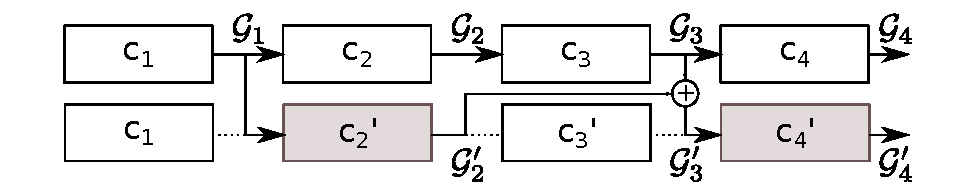
\includegraphics[width=10.5cm]{graphics/eval.pdf}\\[-5mm]
  \caption{Evaluation logic for the example notebook in \Cref{fig:exampleNotebook}.  Edges are labeled with global scope versions.  Cells that are (re-)evaluated are highlighted, dotted lines represent simulated state flow.}
  \label{fig:exampleEval}
\end{wrapfigure}
%%%%%%%%%%%%%%%%%%%%%%%%%%%%%%%%%%%%%%%%
If workflow $\notebook$ is modified by replacing a cell $\nbcell_i$ with a cell $\nbcell_i'$ (denoted as $\notebook[\nbcell_i \backslash \nbcell_i']$), we need to obtain the updated scope $\evalnb{\notebook[\nbcell_i \backslash \nbcell_i']}$. Of course this can be achieved by evaluating $\notebook[\nbcell_i \backslash \nbcell_i']$.
% In lieu of naively re-evaluating the notebook from scratch,
However, to improve performance,  Vizier attempts to update the output of $\evalnb{\notebook}$ by only re-evaluating a subset of the cells.
First, observe that $\globalscope_1, \ldots, \globalscope_{i-1}$ are independent of $\nbcell_i$; and remain unchanged if $\nbcell_i$ is modified.
It is still necessary to have $\globalscope_{i-1}$ to evaluate $\nbcell_i'$; so Vizier caches all intermediate global scopes after evaluating each workflow revision.

% \begin{figure}
%   \centering
%   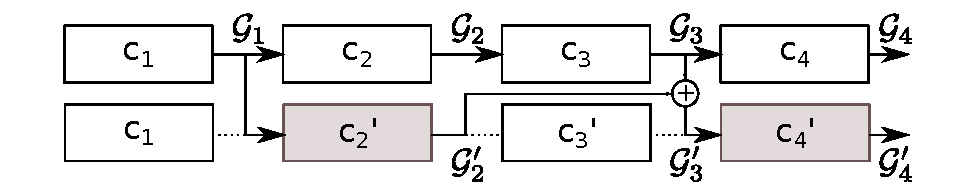
\includegraphics[width=0.7\textwidth]{graphics/eval.pdf}
%   \caption{Evaluation logic for the example notebook in \Cref{fig:exampleNotebook}.  Edges are labeled with global scope versions.  Cells that are (re-)evaluated are highlighted, dotted lines represent simulated state flow.}
%   \label{fig:exampleEval}
% \end{figure}

Naively, we have to still re-evaluate $\nbcell_{i+1}, \ldots, \nbcell_{N}$ using the new scope produced by $\nbcell_i'$. Let us denote the scopes produced by this evaluation as
$\globalscope_{i+1}', \ldots, \globalscope_{n}$.
% $\outputval_{i+1}', \ldots, \outputval_{N}'$.
Vizier uses the readsets $\readset_{\globalscope, i+1}, \ldots, \readset_{\globalscope, N}$, to identify cells $\nbcell_{j}$ for which the same output (artifact versions written by the cell) in $\evalnb{\notebook[\nbcell_i \backslash \nbcell_i']}$ is guaranteed. 
Denote by $\changeset(\globalscope, \globalscope') = \{ k |  \globalscope(k) \neq \globalscope'(k)\}$ the names of artifacts that differ between $\globalscope$ and $\globalscope'$. 
We have to re-execute cell $\nbcell_{i+1}$ if an artifact read by $\nbcell_{i+1}$ has changed, which is the case if $\changeset(\globalscope_i, \globalscope_i') \cap \readset_{\globalscope,i+1} \neq \emptyset$. If $\nbcell_{i+1}$ needs to be re-executed, then we set $\globalscope_{i+1}' = \nbcell_{i+1}(\globalscope_{i}')$. Otherwise, we generate $\globalscope_{i+1}$ by merging the changes made by $\nbcell_{i+1}$ in $\notebook$ to $\globalscope_{i}$ into $\globalscope_{i}'$. That is, for all artifacts $k$ we set
$\globalscope_{i+1}'(k) =   \globalscope_{i+1}(k)$ if $k \in \changeset(\globalscope_i, \globalscope_{i+1})$
and $\globalscope_{i+1}'(k) = \globalscope_{i}'(k)$ otherwise.
% begin{cases}
%   \globalscope_{i+1}(k) &\;\;\;\text{\textbf{if}}\,k \in \changeset(\globalscope_i, \globalscope_{i+1})\\
%   \globalscope_{i}'(k) &\;\;\;\text{\textbf{otherwise}}\\
% \end{cases}$$
 The same approach is applied to decide whether to evaluate or skip the remaining cells in $\notebook[\nbcell_i \backslash {\nbcell_i}']$.


% We formalize a global scope $\globalscope = \{ k_1 \rightarrow v_1, k_2 \rightarrow v_2, \ldots \}$ as a total mapping from an infinite alphabet of variable names $k \in \variabledomain$ to a set of domain values $v \in \valuedomain \cup \{\undefinedval\}$.
% The distinguished symbol $\undefinedval$ denotes an ``undefined'' value, and we assume that finitely many elements of $\variabledomain$ are mapped to non-$\undefinedval$ values (i.e., that $\globalscope$ has finite support).
% Denote by $\keyset(\globalscope) = \{ k | (k \rightarrow v) \in \writeset \wedge v \neq \undefinedval\}$ the keys of the finite support of $\globalscope$.
% Denote by $\changeset(\globalscope, \globalscope') = \{ k |  \globalscope(k) \neq \globalscope'\}$ the change set between $\globalscope$ and $\globalscope'$.

% Given the newly computed $\globalscope_i'$, we want to know if $\nbcell_{i+1}$ needs to be evaluated as well;
% If $\nbcell_{i+1}(\globalscope_i') = (\globalscope_{i+1}', \readset_{i+1}', \outputval_{i+1}')$, we can avoid re-evaluating $\nbcell_{i+1}$ if we can prove that $\outputval_{i+1} = \outputval_{i+1}'$.
% Under the assumption that $\nbcell_{i+1}$ is deterministic with respect to inputs $\readset_{i+1}$, we can guarantee that $\outputval_{i+1} = \outputval_{i+1}'$ when $\readset_{i+1} \cap \changeset(\globalscope_{i}, \globalscope_{i}')$ is empty.
% If we do not need to re-evaluate $\nbcell_{i+1}$, we can reconstruct its output by considering how the original evaluation affected the scope: the write set $\writeset_{i+1} = \changeset(\globalscope_{i}, \globalscope_{i+1})$.
% Concretely $\outputval_{i+1}' = \outputval_{i+1}$, $\readset_{i+1}' = \readset_{i+1}$ and
% $$\globalscope_{i+1}'(k) = \begin{cases}
% \globalscope_{i+1}(k) \textbf{ if } k \in \writeset_{i+1}\\
% \globalscope_{i}'(k) \textbf{ otherwise}
% \end{cases}$$
% \noindent The remaining cells of the notebook are processed in a like manner.

 %%%%%%%%%%%%%%%%%%%%%%%%%%%%%%%%%%%%%%%%%%%%%%%%%%%%%%%%%%%%%%%%%%%%%%%%%%%%%%%%
\begin{exam}
  \Cref{fig:exampleEval} continues the running example from \Cref{ex:introduction}.
  The user has replaced the initial version of cell $\nbcell_2$ with an updated version ${\nbcell_2}'$.
  The global scope produced by preceding cells ($\globalscope_1$) may be re-used unchanged to evaluate ${\nbcell_2}'$, producing scope $\globalscope_2'$.
  $\changeset(\globalscope_2, \globalscope_2')$ is the \lstinline{data} artifact, but the readset of $\nbcell_3$ is empty, and so this cell does not need to be re-evaluated.
  Instead $\globalscope_3'$ is derived by merging variables the cell previously changed (i.e., $\changeset(\globalscope_2, \globalscope_3)$) into the current global scope.
  Finally, Vizier identifies that an element of $\readset_{\globalscope,4}$ (the \lstinline{data} variable) has changed between $\globalscope_3$ and $\globalscope_3'$, necessitating a re-evaluation of cell 4.
\end{exam}
 %%%%%%%%%%%%%%%%%%%%%%%%%%%%%%%%%%%%%%%%%%%%%%%%%%%%%%%%%%%%%%%%%%%%%%%%%%%%%%%%

% \mypara{Frozen Cells}
% Vizier allows users to ``freeze'' cells, temporarily replacing them with no-op commands, but preserving all user-interface elements (including cell outputs), and allowing the cell to be easily re-inserted into the notebook.
% This allows users to quickly disable cells with transient purposes (e.g., sampling cells), or avoid triggering expensive computations while working on an earlier part of the notebook.

% \begin{figure}
%   \centering
%   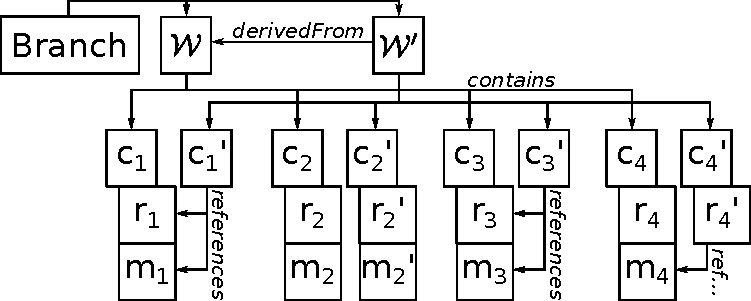
\includegraphics[width=0.45\textwidth]{graphics/history.pdf}\\[-3mm]
%   \caption{History for the running example, assuming cell B was changed as in \Cref{fig:exampleEval}.}
%   \label{fig:exampleHistory}
% \end{figure}

%%%%%%%%%%%%%%%%%%%%%%%%%%%%%%%%%%%%%%%%%%%%%%%%%%%%%%%%%%%%%%%%%%%%%%%%%%%%
%%%%%%%%%%%%%%%%%%%%%%%%%%%%%%%%%%%%%%%%%%%%%%%%%%%%%%%%%%%%%%%%%%%%%%%%%%%%
\subsection{Versioning Workflows}
\label{sec:vizier-history}

%%%%%%%%%%%%%%%%%%%%%%%%%%%%%%%%%%%%%%%%
\begin{wrapfigure}[10]{r}[0pt]{8cm}
  \centering
  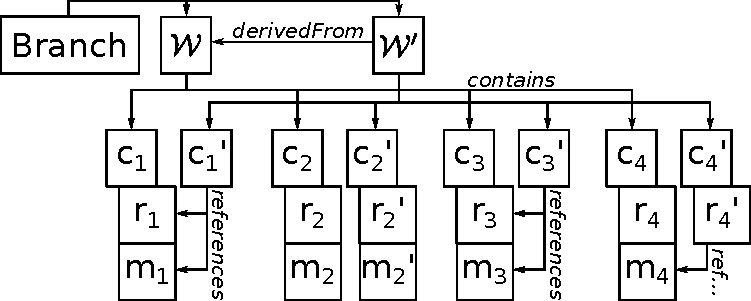
\includegraphics[width=0.45\textwidth]{graphics/history.pdf}\\[-3mm]
  \caption{History for the running example, assuming cell 2 was changed as in \Cref{fig:exampleEval}.}
  \label{fig:exampleHistory}
\end{wrapfigure}
%%%%%%%%%%%%%%%%%%%%%%%%%%%%%%%%%%%%%%%%
Vizier maintains a branching history of the evolution of the notebook.
% We use the term workflow ($\workflow = c_1, \ldots, c_N$) to denote a single state of the notebook.
A cell is further subdivided into (i) \textbf{cell metadata} ($c_i$) that is unique to the workflow (e.g., timestamps and execution status), (ii) \textbf{results} ($r_i$) of executing the cell, and (iii) a \textbf{module} ($m_i$) describing the command executed in the cell.
The latter two components (results and modules) may be shared across workflows.
% In other words, a single cell object acts as a many-to-many-to-many (i.e., 3-ary) relationship between workflow, module, and result entities.
A module object describes the command to be evaluated in a cell.  
This includes its type (e.g., Python or Scala script; SQL query; or one of the graphical widgets), as well as any parameters to the command (e.g., the script itself, or the artifact name to materialize query results as). 
A results object stores references to versions of artifacts in the artifact store created by the execution of the cell. 
We do not materialize the full global scope after each cell, but rather only the changes made to the global scope by the cell (i.e., the cell's write set). 
Any global scope $\globalscope_i$ can be reconstructed from the preceding write sets.

% A results object consists of three items: (i) Messages output by the cell (i.e., $\outputval$), (ii) The cell's readset as a list of name/artifact pairs, and (iii) The cell's writeset as a list of name/artifact pairs.
% Deletion is encoded by writing the distinguished value \texttt{null} to a name.
% As a performance optimization, name/artifact pairs do not embed the artifact literal, but rather a unique artifact identifier.
% This allows for efficient equivalence testing, while avoiding duplication; For example, a ``copy artifact" instruction only needs to clone the artifact identifier under a new name, and not the entire artifact.

% \mypara{Global scope}
% Note that the organizational structure used to persist history information differs from the global scope model used to reason about cell re-use.
% However, the two representations are equivalent.
% Denote by $m_1 \circ m_2$ the right-preferenced composition of \emph{partial} maps $m_1$ and $m_2$ as follows:
% $$m_1 \circ m_2 = \{ k\rightarrow v | (k \rightarrow v) \in m_1 \wedge \not\exists v' \text{ s.t. } (k \rightarrow v') \in m_2 \} \cup m_2$$
% Any global scope $\globalscope_N$ can be recovered by composing the preceding writesets: $\globalscope_N = \globalscope_0 \circ \writeset_1 \circ \ldots \circ \writeset_N$


\begin{exam}
 \Cref{fig:exampleHistory} continues our running example, which in our new terminology is a single branch comprised of two workflows $\workflow_1$ and $\workflow_2$.
  Both notebooks are comprised of four cell objects each.
  Cells 1, 3, and 4 were unchanged between workflows, and so the corresponding cell objects for $\workflow_2$ reference the same module description object as the corresponding cell for $\workflow_1$, while the module descriptions referenced by $\nbcell_2$ and ${\nbcell_2}'$ differ.
  Cells 1 and 3 do not need to be re-evaluated, and so can share their result objects, while Cells 2 and 4 both require re-evaluation and create new result objects.
\end{exam}

%%%%%%%%%%%%%%%%%%%%%%%%%%%%%%%%%%%%%%%%%%%%%%%%%%%%%%%%%%%%%%%%%%%%%%%%%%%%%%%%
\mypara{Workflow and Branch History}
Similar to version control systems like git, each workflow version in Vizier stores a reference to the workflow version it was derived from.
% The difference between workflow versions can be computed by comparing the sequence of modules referenced by the workflow's cells; but simple summary information including the type of change (insert, delete, update) and the affected module (if appropriate) is cached with the workflow object.
A branch is an append-only sequence of workflow versions. % with associated metadata (e.g., a branch name).
The branch contains a reference to the most recent workflow version in the branch. % prior versions are tracked through the series of derived-from references in the workflows themselves.
A new branch may be created from any existing workflow version, including a historical one.

%%%%%%%%%%%%%%%%%%%%%%%%%%%%%%%%%%%%%%%%%%%%%%%%%%%%%%%%%%%%%%%%%%%%%%%%%%%%
%%%%%%%%%%%%%%%%%%%%%%%%%%%%%%%%%%%%%%%%%%%%%%%%%%%%%%%%%%%%%%%%%%%%%%%%%%%%
\subsection{Parallel Scheduler}\label{sec:vizier-scheduler}

The evaluation model presented in \Cref{sec:vizier:eval} relies exclusively on \textit{dynamic provenance}, where Vizier is informed about the readset and writeset of a cell at runtime when the cell accesses artifacts through Vizier's API.
% that assist in determining whether a cell needs to be re-evaluated.
However, dynamic provenance is not always sufficient.
For example, Vizier evaluates cells in parallel where possible, but dynamic provenance is not available until the cell has already been evaluated.
Static provenance, which can derive a cell's read and write sets through static dataflow analysis of its source code, can be computed upfront.
However, static dataflow analysis is of necessity an approximation for some cell types; language features like control flow and dynamic code evaluation can lead to over- (or under-) estimates of the cell's read and write sets. % , especially with respect to a specific global scope.
Vizier uses a novel approach which refines static provenance at runtime using dynamic provenance~\cite{DG22}.

Fundamentally, Vizier's scheduler needs to assign each cell in a running workflow to one of four lifecycle stages: (i) \textbf{DONE} when the cell has a valid result object, (ii) \textbf{PENDING} when the cell depends (directly or transitively) on a cell that does not have a result object, and (iii) \textbf{RUNNING} when the cell's dependencies have a valid result object but the cell itself does not.
We further distinguish as (iv) \textbf{STALE} those cells in the \textbf{PENDING} stage for which we can conclusively determine that re-evaluation is required.
% Lifecycle stage transitions are monotonic.

To manage lifecycle transitions, Vizier's scheduler relies on a combination of static and dynamic provenance~\cite{DG22}.
It uses static provenance to generate an over-approximation on the read and write dependencies of a cell\footnote{As we argue in~\cite{DG22}, to deal with languages that support dynamic code evaluation such as Python, it would be necessary to allow under-approximations of read and write sets (missed data dependencies) and compensate for them at runtime. However, this not implemented in Vizier yet; attempts to dynamically read variables not in the maximal readset are flagged as errors.}.
  % Vizier does not presently support purely dynamic dependencies through e.g., dynamic code evaluation.  A read or write access on a variable not discovered through static analysis triggers an execution error.}.
Accordingly, the scheduler tracks an over-approximation of the read and writesets at each step of the workflow, and refines them when the execution of cell finishes and we know its precise read and write set. 
This approximation is used by Vizier's scheduler to omit cells from re-execution or schedule them for parallel execution if we can determine that it is safe to do so based on these over-approximations.

% Approximate global scopes generalize our prior definition of a global scope by extending the value domain to include the value $\unknownval$, denoting an unresolved value (i.e. variables in an approximate global scope are drawn from $\valuedomain \cup \{\undefinedval, \unknownval\}$).
% Like a regular global scope, an approximate global scope is derived by concatenating writesets ($\globalscope_i = \globalscope_{i-1} \circ \writeset_i$).
% However, if the cell is in a lifecycle stage other than \textbf{DONE}, its previous writeset is not valid.
% Instead, Vizier uses static analysis to derive an upper bound on the writeset $\writeset_{\max} \subseteq \variabledomain$, the maximal set of variables that the cell is allowed to write to.
% When the cell's writeset is not (or may not be) valid, the approximate global scope is instead updated by making each element of $\writeset_{\max}$ an unknown:
% $\globalscope_{i} = \globalscope_{i-1} \circ \{ k \rightarrow \unknownval | k \in \writeset_{\max, i} \}$

% \Cref{alg:lifecycleStage} explains how Vizier derives the lifecycle stage of a cell from the global scope emitted by the preceding cell, the cell's readset (if it exists), and the bound on the readset derived from static analysis.
% The first consideration is whether the cell's prior result object is still valid.
% If there is no prior result object (e.g., because the cell is newly inserted), or if the prior result object is definitely invalid (i.e., because a previously read value was definitely overwritten by a re-evaluated cell), the cell must be re-evaluated.
% What remains is whether the cell can be immediately evaluated (all variables in the upper bound on the readset are defined), or not.

% \begin{algorithm}
% \caption{\lstinline{lifecycle_stage}($\globalscope$, $\readset$, $\readset_{\max}$)}
% \label{alg:lifecycleStage}
% \begin{algorithmic}
%   \REQUIRE{$\globalscope$: The approximate global scope from the prior cell.}
%   \REQUIRE{$\readset$: Either a partial map from $\variabledomain$ to $\valuedomain$ denoting the actual read set if one exists, or $\unknownval$ if the cell is new.}
%   \REQUIRE{$\readset_{\max}$: A set over $\variabledomain$, denoting the statically derived upper bound on the cell's read set.}
%   \ENSURE{$\ell$: The current lifecycle stage of the cell.}
%   \IF{$\readset = \unknownval$ or there exists a $(k \rightarrow v) \in \readset$ such that $\globalscope(k) \neq \unknownval$ and $\globalscope(k) \neq v$}
%     \IF{there exists a $k \in \readset_{\max}$ such that $\globalscope(k) = \unknownval$}
%       \STATE $\ell = \textbf{STALE}$
%         \COMMENT{The cell needs to be re-evaluated, but is missing a dependency}
%     \ELSE
%       \STATE $\ell = \textbf{RUNNING}$
%         \COMMENT{The cell needs to be re-evaluated, and is ready to run}

%     \ENDIF
%   \ELSIF{there exists a $(k \rightarrow v) \in \readset$ where $\globalscope(k) = \unknownval$}
%     \STATE $\ell = \textbf{PENDING}$
%       \COMMENT{The cell may not need re-evaluation, but we don't know yet.}
%   \ELSE
%     \STATE $\ell = \textbf{DONE}$
%       \COMMENT{We can guarantee that the cell does not need re-evaluation.}
%   \ENDIF
% \end{algorithmic}
% \end{algorithm}

% When a cell transitions into the \textbf{RUNNING} state, the scheduler starts the corresponding cell.
% When the cell finishes, it has a state that matches the preceding global state, and transitions into the \textbf{DONE} state.

%%% Local Variables:
%%% mode: latex
%%% TeX-master: "../2022_IEEE_DEB_Vizier"
%%% End:
% %!TEX root=../2022_IEEE_DEB_Vizier.tex
\section{Microkernel Notebooks}
As we outline above, a typical computational notebook relies on a kernel, a long-lived interpreter for a scripting language for a scripting language like python that retains the notebook's intermediate state.
When a cell is executed by the user, its contents are evaluated by the long running interpreter; the interpreter's state changes, and any output produced by the cell (e.g., console logs, charts, or maps) is displayed alongside the cell.
This behavior is independent of the order in which the cell appears in the notebook: The user may return to an earlier cell and modify it, but this cell is simply run against the current state of the interpreter.

Although this design allows users to revise cells in the notebook without being forced to re-run all of the notebooks code from scratch, it does pose several problems.
Most notably that it forces users to reason about the internal state of the kernel, for example by manually adopting a single static assignment variable allocation pattern.
Second, it also requires users to manually keep track of how different notebook cells relate to one-another; When a cell is modified, other cells that depend on it may also need revision.
Finally, in this design, persistence (e.g., of the results of a slow-running computation) must be managed entirely by the user.
Moreover, it is up to the user to manually manage this state to ensure consistent versioning, and portability.

One class of systems including Vizier~\cite{BS20,BB19} and Nodebook address these challenges by checkpointing global notebook state in between cell executions and restoring it when a cell is re-executed.
Thus, the cell is always evaluated on the state version emitted by the preceding cell, and changes to the state can be identified so that subsequent cells that depend on modified outputs can be re-evaluated.
This model 


\begin{itemize}
	\item Standard API for interacting with notebook state facilitates multi-modality
	\begin{itemize}
		\item No $N^2$ problem like for jupyter kernels
		\item Not just notebooks
	\end{itemize}
	\item Typed API allows fine-grained provenance
	\begin{itemize}
		\item Reproducibility
		\item Automatic refresh
		\item No hidden (mystical) dependencies
	\end{itemize}
	\item Challenges:
	\begin{itemize}
		\item Communicating state between kernels
		\item 2-dimensional version model (cell-order vs historical-order <- better name for this exists)
		\item Input/output changes in history vs Operation changes in history
		\begin{itemize}
			\item Vizier: Module vs Cell vs Result
			\item The Vizier execution state-model
		\end{itemize}
		\item Scheduling / Deciding state
	\end{itemize}
\end{itemize}

%%% Local Variables:
%%% mode: latex
%%% TeX-master: "../2022_IEEE_DEB_Vizier"
%%% End:

%!TEX root=../2022_IEEE_DEB_Vizier.tex

\section{Multimodality}
\label{sec:multimodality}

As noted in \Cref{sec:vizier-history}, cells in Vizier implement a variety of different modalities, including scripting languages (e.g., Python, Scala), query languages (e.g., SQL), as well as graphical widgets for data ingestion, transformation, and curation (e.g., Load Dataset, Pivot Table, Repair Key).
We refer to the evaluation logic for each modality as \emph{cell command}.
Each cell in a Vizier workflow identifies the command that should run to evaluate the cell, along with a set of arguments to that command.
For example, the SQL cell (\texttt{sql.query}) takes two arguments: the text of a SQL query, and an optional name to materialize the result table as. In this section, we discuss how these modalities are implemented as cell types in Vizier. % and how they are presented in Vizier's notebook view.

A command is defined by the following methods:
(i) \textbf{schema}: Returns a schema for the arguments the command accepts;
(ii) \textbf{summary(arguments)}: Returns a textual description of the behavior of the command when parameterized by the provided arguments;
(iii) \textbf{dependencies(arguments)}: Returns the over-approximation of the set of names of artifacts read (resp., written) by the cell as parameterized by the provided arguments, or indicates that either or both bounds can not be computed; and
(iv) \textbf{evaluate(arguments, context)}: Evaluates the cell on the command, parameterized by the provided arguments and a context object.

The context object on which commands are evaluated provides a read/write interface to the global scope and a way to emit messages to be displayed alongside the cell in the notebook view.
As we discuss in \Cref{sec:vizier-workflows}, the global scope maps artifact names to artifact versions.
Artifacts are not persisted directly as part of the global scope, but rather are references to our write-only artifact store.\footnote{As mentioned before, artifact versions are immutable in Vizier which simplifies version management. We leave optimizations that selectively violate this policy and update artifacts or store deltas instead of creating full updated versions of artifacts to future work.}
When a cell implementation writes an artifact through the context, the artifact version is serialized and written into the artifact store.
The artifact store assigns the artifact (version) a unique identifier, which is then saved into the scope.
Similarly, to read an artifact, a cell implementation first reads the artifact identifier out of the scope, and then accesses the corresponding artifact version from the store.


%\subsection{Language APIs}
% \mypara{Language APIs}
Cells implementing runtimes for general-purpose languages need to provide users of those languages with a way to interact with the global notebook state.
This entails (i) providing a mechanism to reference the scope and import artifacts within a language-specific format, and (ii) predicting how the user-provided code will interact with the state to bound provenance.

\mypara{Python}
%
Python cells are evaluated in an independent interpreter to avoid concurrency bottlenecks from the global interpreter lock (GIL).
Thus, a key challenge is minimizing the volume of state transferred into and out of each interpreter.
Global scope is lazily loaded by populating the global state with a set of proxy objects, one for each artifact in the scope. % We discuss this based on the example of Python and SQL cells.
%
% When a variable is accessed, the proxy object is ``hydrated'' from the artifact store; From that point on, the proxy object routes all function invocations, property accesses, and operator overload invocations to the hydrated artifact.
% Several small values, including primitive constants and module references, are not compatible with proxy objects, but are small enough to allow them to be hydrated in all cells with negiligible performance cost.
%
Access to the Vizier context for messaging and artifact access occurs through a control bus that, by default, operates over the python process' standard input and output streams.
% Python's normal standard output and error streams are overridden and any output over these channels is converted into control messages; Standard input is disabled for the user-provided script.
Vizier defines a special `show' command within the module to produce structured messages (analogous to placing an item on the last line of a Jupyter cell).
The show command includes support for most Vizier-defined types, matplotlib and bokeh plots, and provides fallbacks using the Jupyter-standard \texttt{\_repr\_html\_} method, or direct stringification as a final resort.
% Vizier also discourages direct file IO by overriding the \texttt{open} command to print a warning message.
%
For predictive dependency tracking, and to identify variables that are modified, Vizier relies on Python's \texttt{ast} module, which provides an introspective compilation and code analysis framework.
Vizier performs lightweight dependency analysis~\cite{DG22} to bound the cell's read and write dependencies.

% identify variables accessed or modified by the cell's code.
% This analysis is used both to bound the read and write dependencies, as well as to determine which variables are exported into the global scope at the end of the cell.
% The AST module is also used to extract code for exported function, module, and class symbols.

\mypara{SQL}
%
SQL cells are parsed and evaluated by Apache Spark.
% Spark provides a convenient global catalog, allowing access to named functions, tables, and other values.
% However, because the specific assignment of names to values varies depending on position in the notebook, relying on the global catalog is not thread-safe.
% Instead,
Vizier intercepts the parsed SQL query AST and manually injects references to the corresponding artifacts --- either datasets or python functions --- where needed.
Spark-provided view name decorators make it possible for the injected views to retain their names from the query, avoiding incomprehensible error messages.
The same injection logic is also used to statically identify exact read and write dependencies.

% Spark has native support for Python User-Defined Functions, but this support is geared towards users accessing spark through its python frontend (\texttt{pyspark}).
% Crucially, it relies on a customized serialization format (\texttt{cloud-pickle}) that is not portable across versions of the serialization library or python.
% When Vizier identifies a reference to a python-defined UDF in a SQL query, it spins up a python interpreter, serializes the UDF, and caches it for subsequent use.

% \mypara{Scala}
% Scala cells are run directly within the Vizier JVM through the Scala reflection toolbox.
% % This feature of Scala allows scala code to be compiled and evaluated at runtime; including support for access to global state.
% % The evaluated code does not have access to local variables; Vizier works around this by passing state in through a thread-local global variable.
% % Like Python cells, Vizier overrides the \texttt{print} and \texttt{println} methods to produce messages rather than standard out.
% At present, access to global state in a scala cell occurs manually; A \texttt{vizierdb} object is created to allow cells to interact with the global scope, or to display more elaborate messages than text allows.
% Similarly, at time of writing, dependency analysis is not yet supported.


%%% Local Variables:
%%% mode: latex
%%% TeX-master: "../2022_IEEE_DEB_Vizier"
%%% End:

% 
\section{The Notebook Modality}\label{sec:notebook-modality}



%%% Local Variables:
%%% mode: latex
%%% TeX-master: "../2022_IEEE_DEB_Vizier"
%%% End:

%!TEX root=../2022_IEEE_DEB_Vizier.tex
\section{Interactive Spreadsheets}
\label{sec:spreadsheets}

A key feature of Vizier is support for direct interaction with artifacts~\cite{BS20}, most notably a spreadsheet-like interface for interacting with Spark Data Frames.
Spreadsheets provide a data exploration experience that is distinct from notebooks.
Users are limited to a single dataset, but have significantly more flexibility when exploring the data.
For example, it is common on small datasets (e.g., under 1000 rows) for users to complete preliminary data cleaning tasks like outlier detection, data integration, repair of typos and outliers, and even some limited computation (e.g., deriving new fields) in a spreadsheet prior to working with the data further (e.g., in a notebook).
Another common use case is manual data entry; The user may enter the entire dataset, or may generate a data entry template (e.g., with a script) and import the resulting file into another tool.

% In both cases, the relationship to the original dataset, and any consequent provenance information is lost.
Vizier's spreadsheet interface is intended to provide a view over a subset of the notebook, allowing users to interact with the dataset in the appropriate modality, while simultaneously preserving workflow provenance  through interactions.
% Furthermore, our goal is to present the spreadsheet as a View over a subset of the notebook.
As the user interacts with the spreadsheet, their edits are reflected in the notebook as new cells.
As the user edits the notebook, their edits are likewise reflected in the spreadsheet --- If the source data frame is updated in the notebook, Vizier attempts to re-apply the user's edits to the updated data.

\mypara{Track Changes as a View}
%
To support bi-directional interaction between spreadsheet and notebook views, Vizier implements a series of specialized cell types that mimic SQL DDL and DML operations, allowing for inserting, deleting, or reordering columns and rows, or for updating individual cell values.
We refer to the operations described by these cell types collectively as the Vizual language~\cite{FG16,BS20}.

Vizual is based on the principle that the user's interactions with a database  can be modeled as views over an original version of the data.
As prior work has shown, a view defined over a table can mimic the effects of any DDL~\cite{DBLP:journals/pvldb/CurinoMZ08} or DML~\cite{DBLP:journals/pvldb/NiuALFZGKLG17} operation applied to the table.
Analogously, each Vizual cell in the notebook uses Spark's standard data frame manipulation language to apply a successive transformation to the dataset that mimics the user's interaction.
To ensure that the spreadsheet remains responsive, a shim layer tentatively injects predicted updates to the user's interactions until the effects of the user's edit are fully applied~(e.g., as \cite{DBLP:conf/icde/GuptaDGUW09}).

In SQL DML, update operations specify target rows by a predicate.
By contrast, operations in a spreadsheet explicitly target specific rows of data, requiring Vizier to assign unique identifiers to each record to encode their order in the spreadsheet\footnote{We assume that the number of columns will remain manageable and reference them purely by name}.
To allow Vizual operations to be replayed as source data changes, these identifiers should remain stable through data transformations.
For derived data, Vizier uses a row identity model similar to GProM's~\cite{DBLP:journals/debu/ArabFGLNZ17} encoding of provenance.
Derived rows, such as those produced by declaratively specified table updates, are identified by an appropriate combination of input tuple identifiers. For example, rows in the output of a join are identified by combining identifiers from the source rows that produced them into a single identifier, and rows in the output of a projection or selection use the identifier of the source row that produced them.
% as follows:
% (i) Rows in the output of a projection or selection use the identifier of the source row that produced them;
% (ii) Rows in the output of a \texttt{UNION ALL} are identified by merging the identifier of the source row with an identifier marking which side of the union the row came from (note that this change renders the \texttt{UNION} operator non-commutative).
% (iii) Rows in the output of a cross product or join are identified by combining identifiers from the source rows that produced them into a single identifier; and (iv) Rows in the output of an aggregate are identified by each row's group-by attribute values.

The remaining challenge is assigning row identifiers to source data, which we want to remain stable through changes to the source data so that spreadsheet operations can be replayed.
Ideally, the data would include a unique identifier that we can leverage; but this is not always the case.
Storing the data in a revision control system~\cite{DBLP:conf/cidr/BhardwajBCDEMP15,DBLP:journals/pvldb/HuangXLEP17}, is not always a viable option~\cite{DBLP:conf/sigmod/AlagiannisBBIA12}.
A more heavyweight approach is to link records across revisions of a dataset~\cite{DBLP:conf/sigmod/YilmazWXNEP18}, but this adds non-negligible overhead to common-case data revisions.
Vizier presently supports persistent identifiers through append- or edit-only revisions by assigning each record a unique identifier based on its position, and a hash of its contents.
This approach has the benefit of being lightweight (it can be applied in a single pass), and resilient.
In contrast to simply using a hash-based identifier, the approach supports duplicate records.
Conversely, solely using a position-based identifier could lead to spreadsheet operations being applied to the wrong row in case of insertions.
%
While techniques for creating identifiers that are stable under updates has been studied extensively for XML databases (e.g., ORDPATH~\cite{DBLP:conf/sigmod/ONeilOPCSW04}) and recently also for spreadsheet views of relational databases~\cite{DBLP:journals/pvldb/BendreSZZCP15}, the main challenge we face in Vizier is how to retain row identity when a new version of a dataset is loaded into Vizier, as opposed to keeping identity consistent once the data is already in the system.
% In this scenario we only have access to two (identifier-free) snapshots of the dataset and no further information on how they relate to each other.

%% Local Variables:
%%% mode: latex
%%% TeX-master: "../2022_IEEE_DEB_Vizier"
%%% End:

%!TEX root=../2022_IEEE_DEB_Vizier.tex

%%%%%%%%%%%%%%%%%%%%%%%%%%%%%%%%%%%%%%%%%%%%%%%%%%%%%%%%%%%%%%%%%%%%%%%%%%%%%%%%
\section{Data Documentation, Error, and Uncertainty Management with Caveats}
\label{sec:data-docum-error}

Like notebook systems, Vizier enables users to document their workflow through markdown cells which do not manipulate artifacts, but simply serve as documentation. 
However, some documentation is specific to individual artifacts, or their component parts (e.g., rows, or columns); 
We would like such documentation to accompany the data as it is transformed~\cite{kumari:2021:cidr:datasense}.
Like other annotation management systems including Mondrian~\cite{GK05} and DBNotes~\cite{bhagwat-05-anmsrd},
Vizier empowers users to annotate data with textual comments. 
However, in contrast to these systems, in Vizier these annotations also have a precise semantics: they encode uncertainty about an attribute value of a row or the existence of a row. 
This is important, because uncertainty arises naturally in most data science pipelines (e.g., because of errors in the data or because of heuristic choices during data cleaning) and if data analysis ignores the uncertainty in the data, it can lead to analysis results that cannot be trusted.
To address this issue, caveats are propagated through operations on dataset artifacts in Vizier using an efficient uncertain query semantics we have developed~\cite{FH19, FH21}. 
Thus, caveats on values and rows in the result of an analysis conducted using Vizier encode information about how data cleaning and curation operations on the data used in the analysis affect the analysis result. 
Furthermore, Vizier's implementation of data cleaning operations introduce caveats to encode information about other possible repairs.

%%%%%%%%%%%%%%%%%%%%%%%%%%%%%%%%%%%%%%%%%%%%%%%%%%%%%%%%%%%%%%%%%%%%%%%%%%%%%%%%
\subsection{Incomplete Databases}
\label{sec:incomplete-databases}

Formally, caveats in Vizier are based on an approximation of incomplete databases. An incomplete database $\pdb = \{D_1, \ldots, D_n\}$ is a set of deterministic databases called possible worlds that encode alternative possibilities for the state of the real world: one possible world corresponds to the actual state of the real world, but we do not know which. 
As an example, consider an analyst that has to find the names of important customers (e.g., who ordered products totaling more than \$500). 
An example instance is shown in \Cref{fig:example-customer-database}. 
A common method for primary key repair is to group rows by their PK values and select one row from each group to be retained. 
However, typically we have insufficient information to know which row is the correct choice and will have to rely on heuristics (e.g., selecting the most recently updated row if this information is available). 
Incomplete databases can be used to model this uncertainty: we create an incomplete database whose worlds are all the repairs of the database violating the constraint~\cite{DBLP:journals/vldb/BeskalesIGG14}.
\Cref{fig:example-customer-database} shows two (out of 4) possible repairs for this dataset.

%%%%%%%%%%%%%%%%%%%%%%%%%%%%%%%%%%%%%%%%
\begin{figure}[t]
  \centering

  \begin{minipage}[b]{0.31\linewidth}
\centering
    \textbf{Customer Relation}\\[3mm]
    %%%%%%%%%%%%%%%%%%%%%%%%%%%%%%%%%%%%%%%%
    \begin{tabular}{c|c|c}
      \thead{cid} & \thead{name} & \thead{total} \\     \hline
      1         & Peter          Petersen        & 1000 \\
      1         & Peter          Petersen        & 950  \\
      2         & Bob            Smith           & 300  \\
      3         & Alice          Smith           & 400  \\
      3         & Alice          Smith           & 600  \\
    \end{tabular}
    %%%%%%%%%%%%%%%%%%%%%%%%%%%%%%%%%%%%%%%%
  \end{minipage}
%
  \begin{minipage}[b]{0.31\linewidth}
\centering
    \textbf{Possible       World           (Repair) $D_1$}\\[3mm]
    %%%%%%%%%%%%%%%%%%%%%%%%%%%%%%%%%%%%%%%
    \begin{tabular}{c|c|c}
      \thead{cid} & \thead{name} & \thead{total} \\       \hline
      1         & Peter          Petersen        & 1000   \\
      2         & Bob            Smith           & 300    \\
      3         & Alice          Smith           & 400    \\
    \end{tabular}
    %%%%%%%%%%%%%%%%%%%%%%%%%%%%%%%%%%%%%%%%
  \end{minipage}
%
  \begin{minipage}[b]{0.31\linewidth}
\centering
    \textbf{Possible       World           (Repqir) $D_2$}\\[3mm]
    %%%%%%%%%%%%%%%%%%%%%%%%%%%%%%%%%%%%%%%
    \begin{tabular}{c|c|c}
      \thead{cid}   & \thead{name} & \thead{total} \\       \hline
      1           & Peter          Petersen        & 1000   \\
      2           & Bob            Smith           & 300    \\
      3           & Alice          Smith           & 600    \\
    \end{tabular}
    %%%%%%%%%%%%%%%%%%%%%%%%%%%%%%%%%%%%%%%%
  \end{minipage}


  %%%%%%%%%%%%%%%%%%%%%%%%%%%%%%%%%%%%%%%%
  \begin{minipage}{0.31 \textwidth}
    \centering
    \textbf{Certain Answers}\\[3mm]
    %%%%%%%%%%%%%%%%%%%%%%%%%%%%%%%%%%%%%%%%
    \begin{tabular}{c}
      \thead{name}\\ \hline
      Peter Petersen \\
    \end{tabular}
    %%%%%%%%%%%%%%%%%%%%%%%%%%%%%%%%%%%%%%%%
  \end{minipage}
  %%%%%%%%%%%%%%%%%%%%%%%%%%%%%%%%%%%%%%%%
  %
  %%%%%%%%%%%%%%%%%%%%%%%%%%%%%%%%%%%%%%%%
  \begin{minipage}{0.31 \textwidth}
    \centering
    \textbf{Answers in $D_1$}\\[3mm]
    %%%%%%%%%%%%%%%%%%%%%%%%%%%%%%%%%%%%%%%%
    \begin{tabular}{c}
      \thead{name}\\ \hline
      Peter Petersen \\
    \end{tabular}
    %%%%%%%%%%%%%%%%%%%%%%%%%%%%%%%%%%%%%%%%
  \end{minipage}
  %%%%%%%%%%%%%%%%%%%%%%%%%%%%%%%%%%%%%%%%
  %
  %%%%%%%%%%%%%%%%%%%%%%%%%%%%%%%%%%%%%%%%
  \begin{minipage}{0.31 \textwidth}
    \centering
    \textbf{Answers in $D_2$}\\[3mm]
    %%%%%%%%%%%%%%%%%%%%%%%%%%%%%%%%%%%%%%%%
    \begin{tabular}{c}
      \thead{name}\\ \hline
      Peter Petersen \\
      Alice Smith\\
    \end{tabular}
    %%%%%%%%%%%%%%%%%%%%%%%%%%%%%%%%%%%%%%%%
  \end{minipage}
  %%%%%%%%%%%%%%%%%%%%%%%%%%%%%%%%%%%%%%%%


  \caption{Example customer database violating the primary key constraint that cid is unique and two possible worlds corresponding to some of the possible repairs of the database achieved by selecting one row among each group of rows with the same primary key value.}\label{fig:example-customer-database}
\end{figure}
%%%%%%%%%%%%%%%%%%%%%%%%%%%%%%%%%%%%%%%%

Typical constraint-repair algorithms will select one repair (one possible world) based on a heuristic like selecting the row whose values are most common in the dataset~\cite{RC17}. For instance, the cleaning algorithm may choose $D_1$ and the user would then evaluate their query (shown below) over $D_1$.

\begin{lstlisting}
                  SELECT name FROM Customer WHERE total > 500;
\end{lstlisting}

%%%%%%%%%%%%%%%%%%%%%%%%%%%%%%%%%%%%%%%%
\begin{wrapfigure}[15]{r}[0pt]{8cm}
  \centering
    % \textbf{UA-DB with Selected Guess $D_1$}\\[3mm]
    %%%%%%%%%%%%%%%%%%%%%%%%%%%%%%%%%%%%%%%
    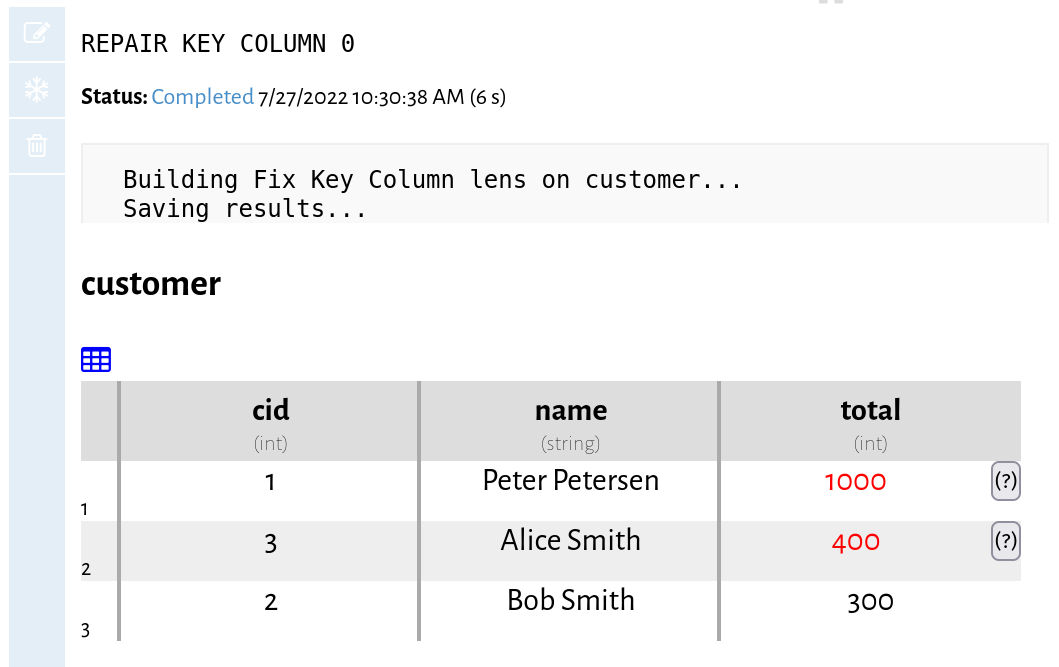
\includegraphics[width=8cm]{graphics/caveatted_data.png}
    % \begin{tabular}{c|c|c|c}
    %   \thead{cid} & \thead{name} & \thead{total} & \\       \hline
    %   1         & Peter          Petersen        & 1000 &   \\
    %   2         & Bob            Smith           & 300  & \rowcaveat  \\
    %   3         & Alice          Smith           & 400  & \rowcaveat  \\
    % \end{tabular}
    %%%%%%%%%%%%%%%%%%%%%%%%%%%%%%%%%%%%%%%%
  \caption{A UB-DB in Vizier encoding $D_1$ with possibly uncertain cells marked with caveats.}\label{fig:ub-db-encoding-d-2-with-p}
\end{wrapfigure}
%%%%%%%%%%%%%%%%%%%%%%%%%%%%%%%%%%%%%%%%
While such heuristics may be quite effective on average and are certainly superior to just randomly selecting a world, it is unavoidable that they fail for some cleaning scenarios. 
An alternative approach called consistent query answering~\cite{B11} takes a conservative stance, instead of selecting one repair, we reason about all possible repairs and only return query answers (the so-called \textit{certain answers}) that are in the query's results for every repair (i.e., are guaranteed to be in the result independent of which repair is correct). 
This approach has the advantage that only correct query answers are returned, but is computationally expensive, may exclude many very likely answers (if they are not 100\% certain), and is not closed (it is not possible to evaluate queries with certain answer semantics over the certain answers of a query).


%%%%%%%%%%%%%%%%%%%%%%%%%%%%%%%%%%%%%%%%%%%%%%%%%%%%%%%%%%%%%%%%%%%%%%%%%%%%%%%%
\subsection{Attribute- and Row-level Caveats and\\ Uncertainty-Annotated Databases}
\label{sec:attribute-row-level}
%
\begin{wrapfigure}[6]{r}[0pt]{8cm}
  \vspace*{-5mm}
  \centering
  \vspace*{-14mm}
  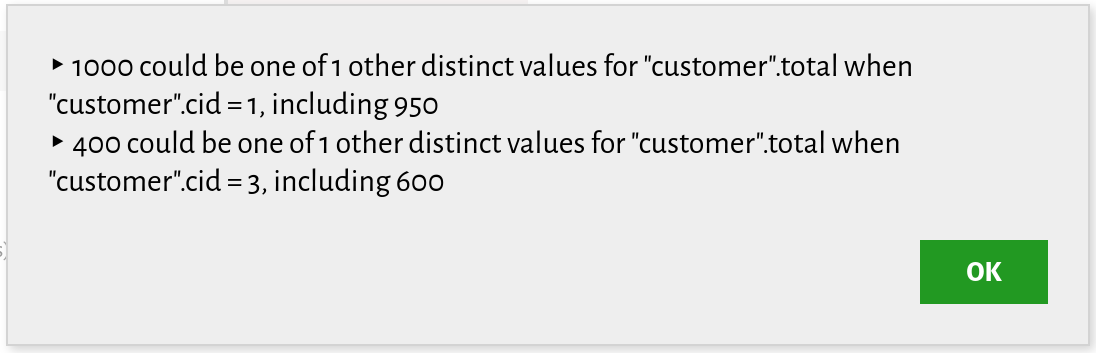
\includegraphics[width=8cm]{graphics/caveats.png}
  \caption{Caveats annotating the relation $D_1$}
\end{wrapfigure}
%


For Vizier, we developed an uncertain data model called
uncertainty-annotated databases~\cite{FH19} that annotates one
possible world (the so-called \textit{selected-guess world}) with an under-approximation  of certain answers (if we claim that a row is certain, then it is certain) that can be computed efficiently. This is encoded by annotating a subset of a dataset's rows with row-level caveats to mark them as not being certain.  The reason that we use an under-approximation is to be able to evaluate complex queries (full relational algebra including aggregation) efficiently (with PTIME data complexity and small overhead over deterministic query processing). Furthermore, attribute-level caveats are used to mark attribute values as uncertain (they may not be the same in every possible world) which is similar in nature to certain answers with nulls~\cite{L16a}.

% %%%%%%%%%%%%%%%%%%%%%%%%%%%%%%%%%%%%%%%%
% \begin{figure}[t]
%   \centering

% \begin{minipage}[b]{0.31\linewidth}
% \centering
%     \textbf{UA-DB with Selected Guess $D_1$}\\[3mm]
%     %%%%%%%%%%%%%%%%%%%%%%%%%%%%%%%%%%%%%%%
%     \begin{tabular}{c|c|c|c}
%       \thead{cid} & \thead{name} & \thead{total} & \\       \hline
%       1         & Peter          Petersen        & 1000 & \rowcaveat  \\
%       2         & Bob            Smith           & 300  & \rowcaveat  \\
%       3         & Alice          Smith           & 400  & \rowcaveat  \\
%     \end{tabular}
%     %%%%%%%%%%%%%%%%%%%%%%%%%%%%%%%%%%%%%%%%
%   \end{minipage}

%   \caption{UB-DB encoding $D_2$ with possibly uncertain rows marked with caveats (aster ix).}\label{fig:ub-db-encoding-d-2-with-p}
% \end{figure}
% %%%%%%%%%%%%%%%%%%%%%%%%%%%%%%%%%%%%%%%%

%%%%%%%%%%%%%%%%%%%%%%%%%%%%%%%%%%%%%%%%%%%%%%%%%%%%%%%%%%%%%%%%%%%%%%%%%%%%%%%%
% \subsection{Queries over Uncertainty-Annotated Databases}
% \label{sec:uncert-annot-datab}

% In~\cite{FH19} we introduced a query semantics for UA-DBs that

% %%%%%%%%%%%%%%%%%%%%%%%%%%%%%%%%%%%%%%%%%%%%%%%%%%%%%%%%%%%%%%%%%%%%%%%%%%%%%%%%
% \subsection{Implementation in Spark}
% \label{sec:implementation-spark}





%%% Local Variables:
%%% mode: latex
%%% TeX-master: "../2022_IEEE_DEB_Vizier"
%%% End:


%%%%%%%%%%%%%%%%%%%%%%%%%%%%%%%%%%%%%%%%%%%%%%%%%%%%%%%%%%%%%%%%%%%%%%%%%%%%%%%%
\section{Conclusions and Future Work}
\label{sec:conclusions}

In this paper, we have made the case for a multi-modal data science platform built on top of an incremental, data-centric workflow engine and have introduced the reader to Vizier, our system implementing this vision. 
Because each modality (notebooks, spreadsheets, the caveat view, etc\ldots) is a ``view'' interacting with the same underlying workflow and datasets, it is easy to extend the system to support new interaction paradigms in the future.  Building our system so that cells execute in isolation and only interact through dataflow makes it easy to add new cell types to the system, because we only have to worry about the interaction of the new cell type with  data artifacts. 
Thus, adding support for other interaction modalities (e.g., new programming languages) into the system is straight-forward: we implement a new cell type and an API to access Vizier artifacts from within the modality.

As demonstrated in recent preliminary work, having a scheduler that revises its schedule based on dependencies discovered at runtime and using static dataflow analysis, we can execute notebook cells in parallel and avoid re-executing cells that are guaranteed not to change during automatic refresh.
Significantly more opportunities for avoiding work exist, in particular by leveraging Vizier's standardized representation of artifacts.
For example, by representing updates to dataset artifacts as change sets, existing approaches for incremental view maintenance can reduce the runtime overhead of recomputing workflow steps, as well as the space costs of preserving multiple artifact versions. Another interesting direction for future work is to study incremental maintenance of workflow results when the definition of a workflow step changes. This is an novel variation of the traditional incremental view maintenance problem where we have to update the result based on a change to the query rather than based on a change to the data.

Similarly, standard representations of artifacts can be used to help users better understand the outputs of their workflows.
For example, numerous efforts have explored causal explanations in database query results (\cite{DBLP:conf/sigmod/KanagalLD11,DBLP:journals/pvldb/MeliouGMS11,DBLP:journals/pvldb/MeliouRS14,DBLP:journals/ftdb/GlavicMR21}, and explainability in machine learning has recently become an area of active research.
For such techniques to be truly valuable, they need to operate across artifact types. For example, what would it take to link a sudden change in predictions made by a model to the addition of a new category in source data five transformations removed from the model training step. With Vizier's uncertainty model and provenance tracking we lay the ground work to develop methods for generating explanations that span multiple steps in a workflow. 

Finally, we note that Vizier provides a ``ground-up'' approach to stitching different interaction modalities into a single workflow.
Tools implemented as views over Vizier's workflow model seamlessly interact with each other, with coarse-grained provenance, reactive cell execution, and repeatability/reproducibility.
However, these capabilities are limited to a single Vizier instance, and are of limited value to already existing tools.
An important open challenge is the design of a federated infrastructure for data analytics workflows, allowing multiple Vizier instances or unrelated tools to interoperate.


%%%%%%%%%%%%%%%%%%%%%%%%%%%%%%%%%%%%%%%%%%%%%%%%%%%%%%%%%%%%%%%%%%%%%%%%%%%%%%%%
% ACKNOWLEDGEMENTS
\mypara{Acknowledgements} This work was supported by NSF Awards ACI-1640864, IIS-1750460, IIS-1956149, and IIS-2125516. % and \ldots

%%%%%%%%%%%%%%%%%%%%%%%%%%%%%%%%%%%%%%%%%%%%%%%%%%%%%%%%%%%%%%%%%%%%%%%%%%%%%%%%
% BIBLIOGRAPHY
%\bibliographystyle{abbrv}
%\bibliography{2022_IEEE_DEB_Vizier.bib}

\documentclass[11pt]{article}

\usepackage{deauthor,times,graphicx}
\usepackage{color,colortbl}
% \usepackage[dvipsnames]{xcolor}
% \usepackage{hyperref}
\usepackage{amsmath}
\usepackage{amssymb}
\let\proof\relax
\let\endproof\relax
\usepackage{amsthm}
\usepackage{cleveref}
\usepackage{wrapfig}
\usepackage{url}
\usepackage{stmaryrd,amssymb}
\usepackage{listings}
\usepackage{algorithm}
% \usepackage[noend]{algorithmic}
\usepackage{fancybox}


%%%%%%%%%%%%%%%%%%%%%%%%%%%%%%%%%%%%%%%%
% Theorems, Definitions, Examples
%%%%%%%%%%%%%%%%%%%%%%%%%%%%%%%%%%%%%%%%
\newtheorem{theo}{Theorem}
\numberwithin{theo}{section}
\newtheorem{lem}[theo]{Lemma}
\newtheorem{propo}[theo]{Proposition}
\newtheorem{coll}[theo]{Corollary}
\newtheorem{exam}{Example}
\numberwithin{exam}{section}
\newtheorem{defi}{Definition}
\numberwithin{defi}{section}


%%%%%%%%%%%%%%%%%%%%%%%%%%%%%%%%%%%%%%%%%%%%%%%%%%%%%%%%%%%%%%%%%%%%%%%%%%%%%%%%
\usepackage{todonotes}
\newcommand{\BG}[1]{\todo[inline]{\textbf{Boris:} #1}}
\newcommand{\OK}[1]{\todo[inline]{\textbf{Oliver:} #1}}
\newcommand{\JF}[1]{\todo[inline]{\textbf{Juliana:} #1}}
\newcommand{\MB}[1]{\todo[inline]{\textbf{Mike:} #1}}

\newcommand{\jfedit}[1]{\textcolor{red} {#1}}


%%%%%%%%%%%%%%%%%%%%%%%%%%%%%%%%%%%%%%%%%%%%%%%%%%%%%%%%%%%%%%%%%%%%%%%%%%%%%%%%
% OUR SETUP
\newcommand{\mypara}[1]{\medskip\noindent\textbf{{#1}.}}

\ifdefined\thead
\else
  \newcommand{\thead}[1]{\textbf{#1}}
\fi
\newcommand{\rowcaveat}{\textbf{\textcolor{red}{$\ast$}}}
\newcommand{\pdb}{\mathcal{D}}

%%%%%%%%%%%%%%%%%%%%%%%%%%%%%%%%%%%%%%%%%%%%%%%%%%%%%%%%%%%%%%%%%%%%%%%%%%%%%%%%
% DOCUMENT
\begin{document}

%%%%%%%%%%%%%%%%%%%%%%%%%%%%%%%%%%%%%%%%%%%%%%%%%%%%%%%%%%%%%%%%%%%%%%%%%%%%%%%%
% LST DEFS

%%%%%%%%%%%%%%%%%%%%%%%%%%%%%%%%%%%%%%%%
% Colors
%%%%%%%%%%%%%%%%%%%%%%%%%%%%%%%%%%%%%%%%
\definecolor{lstpurple}{rgb}{0.5,0,0.5}
\definecolor{lstred}{rgb}{1,0,0}
\definecolor{lstreddark}{rgb}{0.7,0,0}
\definecolor{lstredl}{rgb}{0.64,0.08,0.08}
\definecolor{lstmildblue}{rgb}{0.66,0.72,0.78}
\definecolor{lstblue}{rgb}{0,0,1}
\definecolor{lstmildgreen}{rgb}{0.42,0.53,0.39}
\definecolor{lstgreen}{rgb}{0,0.5,0}
\definecolor{lstorangedark}{rgb}{0.6,0.3,0}
\definecolor{lstorange}{rgb}{0.75,0.52,0.005}
\definecolor{lstorangelight}{rgb}{0.89,0.81,0.67}
\definecolor{lstbeige}{rgb}{0.90,0.86,0.45}


% Declare bold typewriter font with Computer Modern
\DeclareFontShape{OT1}{cmtt}{bx}{n}{<5><6><7><8><9><10><10.95><12><14.4><17.28><20.74><24.88>cmttb10}{}

%%%%%%%%%% SQL + proveannce listing settings
\lstdefinestyle{psql}
{
tabsize=2,
basicstyle=\small\upshape\ttfamily,
language=SQL,
morekeywords={PROVENANCE,BASERELATION,INFLUENCE,COPY,ON,TRANSPROV,TRANSSQL,TRANSXML,CONTRIBUTION,COMPLETE,TRANSITIVE,NONTRANSITIVE,EXPLAIN,SQLTEXT,GRAPH,IS,ANNOT,THIS,XSLT,MAPPROV,cxpath,OF,TRANSACTION,SERIALIZABLE,COMMITTED,INSERT,INTO,WITH,SCN,UPDATED,PARTITION,BY,PRECEDING,FOLLOWING,CURRENT,ROW,ROWS,RANGE,GROUPING,SETS,CUBE,ROLL,UP},
extendedchars=false,
keywordstyle=\bfseries,
mathescape=true,
escapechar=@,
sensitive=true
}


%%%%%%%%%% SQL + proveannce listing settings - colorful version
\lstdefinestyle{psqlcolor}
{
tabsize=2,
basicstyle=\small\upshape\ttfamily,
language=SQL,
morekeywords={PROVENANCE,BASERELATION,INFLUENCE,COPY,ON,TRANSPROV,TRANSSQL,TRANSXML,CONTRIBUTION,COMPLETE,TRANSITIVE,NONTRANSITIVE,EXPLAIN,SQLTEXT,GRAPH,IS,ANNOT,THIS,XSLT,MAPPROV,OF,TRANSACTION,SERIALIZABLE,COMMITTED,INSERT,INTO,WITH,SCN,UPDATED},
extendedchars=false,
keywordstyle=\bfseries\color{lstpurple},
deletekeywords={count,min,max,avg,sum},
keywords=[2]{count,min,max,avg,sum,first,last,lead,lag,cxpath},
keywordstyle=[2]\color{lstblue},
stringstyle=\color{lstreddark},
commentstyle=\color{lstgreen},
mathescape=true,
escapechar=@,
sensitive=true
}


%%%%%%%%%% DATALOG style
\lstdefinestyle{datalog}
{
basicstyle=\footnotesize\upshape\ttfamily,
language=prolog
}




%%%%%%%%%% listings settings for pseudo code
\lstdefinestyle{pseudocode}
{
  tabsize=3,
  basicstyle=\small,
  language=c,
  morekeywords={if,else,foreach,case,return,in,or},
  extendedchars=true,
  mathescape=true,
  literate={:=}{{$\gets$}}1 {<=}{{$\leq$}}1 {!=}{{$\neq$}}1 {append}{{$\listconcat$}}1 {calP}{{$\cal P$}}{2},
  keywordstyle=\color{lstpurple},
  escapechar=&,
  numbers=left,
  numberstyle=\color{lstgreen}\small\bfseries,
  stepnumber=1,
  numbersep=5pt,
}

% \definecolor{pynotebookcellbg}{RGB}{247,247,247}
\definecolor{pynotebookcellbg}{gray}{0.95}

\lstdefinestyle{pynotebook}
{
  tabsize=3,
  basicstyle=\small\upshape\ttfamily,
  language=python,
  extendedchars=true,
  mathescape=true,
  morekeywords={show,read_csv,read_geojson,groupby,spatial_join,geocode,count},
  keywordstyle=\color{Blue},
  stringstyle=\itshape\color{Sepia},
  identifierstyle=\bfseries\color{OliveGreen},
  escapechar=&,
  numbers=left,
  numberstyle=\tiny\bfseries\ttfamily\color[gray]{0.7},
  stepnumber=1,
  numbersep=5pt,
  frame=single,
  frameround=tttt,
  backgroundcolor=\color{pynotebookcellbg}
}

\lstset{style=psqlcolor}

%%%%%%%%%%%%%%%%%%%%%%%%%%%%%%%%%%%%%%%%%%%%%%%%%%%%%%%%%%%%%%%%%%%%%%%%%%%%%%%%

\newcommand{\tinysection}[1]{
  \medskip \noindent \textbf{#1}.
}

%%%%%%%%%%%%%%%%%%%%%%%%%%%%%%%%%%%%%%%%%%%%%%%%%%%%%%%%%%%%%%%%%%%%%%%%%%%%%%%%
% TITLE AND AUTHORS
\title{The Right Tool for the Job: Data-Centric Workflows in Vizier}
%\title{It's a Notebook, It's a Spreadsheet, \ldots It's Vizier!}

\author{Oliver Kennedy,$^{\star}$~~Boris Glavic,$^{\diamond}$~~Juliana Freire,$^{\dagger}$~~and~~Michael Brachmann$\,^{\star}$\\
$^{\star}$~University at Buffalo, USA\\
$^{\diamond}$~Illinois Institute of Technology, USA\\
$^{\dagger}$~New York University, USA
}

\maketitle

\graphicspath{{submissions/workflow-vizier-glavic/}}

%%%%%%%%%%%%%%%%%%%%%%%%%%%%%%%%%%%%%%%%%%%%%%%%%%%%%%%%%%%%%%%%%%%%%%%%%%%%%%%%
% ABSTRACT
\begin{abstract}
  Data scientists use a wide variety of systems with a wide variety of
  user interfaces such as spreadsheets and notebooks for their data
  exploration, discovery, preprocessing, and analysis
  tasks. % For instance, spreadsheet interfaces are used for manual curation and simple types of analysis; notebook interfaces are used for data preprocessing, analysis, and visualization; and big data platforms, workflow systems, and database systems are used for more advanced querying and for deploying data analysis pipelines that were prototyped using notebooks.
  While this wide selection of tools offers data scientists the
  freedom to pick the right tool for each task, each of these tools
  has limitations (e.g., the lack of
  reproducibility % and automatic refresh of outdated results in
  of
  notebooks), % or the limited support of spreadsheets to specify batch data transformations),
  data needs to be translated between tool-specific formats, and
  common functionality such as versioning, provenance, and dealing
  with data errors often has to be implemented for each
  system. We argue that rather than alternating between task-specific
  tools, a superior approach is to build multiple user-interfaces on top
  of a single incremental workflow / dataflow platform with built-in
  support for versioning, provenance, error \& tracking, and data
  cleaning. We discuss Vizier, a notebook system that implements this
  approach, introduce the challenges that arose in building such a
  system, % , and compare the approach against state-of-the-art systems. Furthermore, we
  and highlight how our work on Vizier lead to novel research in
  uncertain data management and incremental execution of workflows.
\end{abstract}
%%%%%%%%%%%%%%%%%%%%%%%%%%%%%%%%%%%%%%%%%%%%%%%%%%%%%%%%%%%%%%%%%%%%%%%%%%%%%%%%


%%%%%%%%%%%%%%%%%%%%%%%%%%%%%%%%%%%%%%%%%%%%%%%%%%%%%%%%%%%%%%%%%%%%%%%%%%%%%%%%
\section{Introduction}
\label{sec:intro}

Federated Learning (FL) is a distributed machine learning (ML) paradigm that trains a model across a number of participating entities holding local data samples.
% , without exchanging them. 
In this work, we focus on \emph{cross-device} FL that harnesses a large number (up to hundreds of millions) of edge devices with disparate characteristics such as availability, compute, memory, or connectivity
resources~\citep{kairouz2019advances}. %that harnesses potential
% Current applications of FL are designed to scale up to client populations of hundreds of millions or even billions. 
Two challenges to the success of cross-device FL are privacy and scalability. 
FL was originally motivated for improving privacy since data points remain on client devices. 
% and only small model updates were shared to a co-ordinating server.
However, as with other forms of ML, information about training data can be extracted via membership inference or reconstruction attacks on a trained model \citep{carlini2021membership,carlini2020extracting}, or leaked through local updates~\citep{MelisSCS19,geiping2020inverting}. 
Consequently, Secure Aggregation (\SecAgg) protocols were introduced to prevent the server from directly observing individual client updates, which is a major vector for information leakage~\citep{bonavitz2019federated,huba2021papaya}. 
Additional mitigations such as  Differential Privacy (DP) may be required to offer further protection 
against attacks~\citep{dwork2006calibrating,abadi2016deep}, as discussed in Section~\ref{sec:discussion}.
% , as discussed in Section~\ref{sec:discussion}.
%As an additional layer of protection against statistical inference attacks, SecAgg is usually paired with Differential Privacy (DP) \citep{dwork2006calibrating}. To realize the full promise of FL as a privacy-enhancing technology, we need both SecAgg and Differential Privacy.

Ensuring scalability to populations of heterogeneous clients is the second challenge for FL.
% There are many aspects for FL scalability, such as ensuring that model updates can be calculated efficiently 
% by devices with various capabilities and intermittent availability~\citep{bonavitz2019federated}.
% Here, we focus on the communication bottleneck as the primary concern.
Indeed, wall-clock training times are highly correlated with increasing model and batch sizes~\citep{huba2021papaya}, even with recent efforts such as FedBuff~\citep{nguyen2021federated},
% With increasing model and batch sizes, the wall-clock training time increases accordingly~\citep{huba2021papaya}. 
% Despite efforts such as buffered asynchronous aggregation~\cite{nguyen2021federated}, 
and communication overhead between the server and clients dominates model convergence time.
% cross-device FL remains bottlenecked by communication latency between the server and the clients. 
% \karthik{should we mention this paper in a different way? Fedbuff paper doesn't explicitly call out latency as an issue, nor do we run experiments to on async fl ourselves}  \ashkan{I also think the transition can be smoother: first we focus on scalability and billions. Then we say communication is the bottleneck} 
Consequently, compression techniques were used to reduce the communication bandwidth while maintaining model accuracy.
However, a fundamental problem has been largely overlooked in the literature: in their native form, standard compression methods such as scalar quantization and pruning are not compatible with \SecAgg. 
This makes it challenging to ensure both security and communication efficiency.
% at the same time.
% the default method to provide security for client update, 
% presenting an unpleasant dichotomy between security or efficiency. 


% Second, this is the most restricted direction, since upload bandwidth remains more restricted than download. 
% In the US, fixed-line broadband speeds typically achieve a ratio of $3\times$ to $20\times$ more download bandwidth than upload
% bottlenecks remain, and so we seek to reduce the message size of clients by \textit{compression}. 
% Compression has been widely proposed in various ML scenarios, in the form of pruning (removing model parameters) and quantization (reducing fidelity of parameter representation). 
% Indeed, these techniques have been successfully used in FL settings with appreciable improvements in communication while maintaining model accuracy. 
% However, there is a fundamental problem which has been largely overlooked in the literature: in their native form, these compression methods are not compatible with SecAgg, the default method to provide security for client updates. 
% This presents an unpleasant dichotomy: we can have security or efficiency, but not both. 
%
%
% In this paper, we resolve this gap by showing how to modify FL compression techniques to make them security-friendly. We focus on compressing \emph{uplink} updates from clients to the server for two reasons. 
% First, uplink communications are subject to Secure Aggregation protocols to ensure a high security bar, while downlink updates broadcasted by the server are deemed public. 
% Second, upload bandwidth is generally more restricted than download. For instance, according to the most recent FCC report, the ratio of download to upload speeds for DSL/cable providers\footnote{Fixed-line broadband is most relevant since FL is typically restricted to using unmetered connections, usually over Wi-Fi~\citep{huba2021papaya}.} in the US ranges between 3$\times$ to 20$\times$~\citep{fcc-broadband}.
% % This requires some meticulous changes to coordinate clients to use the same global (non-private) hyperparameters, and show that this coordination does not damage model quality. 
% % For the strongest compression methods, we step outside of the SecAgg primitive and propose a new secure primitive, Secure Indexing, which enables the best compression ratios without sacrificing utility. 
% Finally, efficient and secure uplink communication brings several benefits beyond speeding up convergence: 
% lowering communication cost reduces selection bias due to undersampling clients with limited connectivity, improving fairness and inclusivity metrics. 
% It also shrinks the carbon footprint of FL, whose fraction attributable to communication can reach 95\%~\citep{qiu2021first}.
%
%In this paper, w
We address this gap by adapting compression techniques to make them compatible with \SecAgg. We focus on compressing \emph{uplink} updates from clients to the server for three reasons. 
First, uplink communication is more sensitive and so is subject to a high security bar, whereas downlink updates broadcast by the server are deemed public. 
Second, upload bandwidth is generally more restricted than download bandwidth. For instance, according to 
a recent FCC report, 
%the most recent \modif{FCC\footnote{\modif{US Federal Communications Commission.}} report}, 
the ratio of download to upload speeds for DSL and cable providers\footnote{FL is typically restricted to using unmetered connections, usually over Wi-Fi~\citep{huba2021papaya}.} in the US ranges between 3$\times$ to~20$\times$~\citep{fcc-broadband}.
% Fixed-line broadband is most relevant since
% This requires some meticulous changes to coordinate clients to use the same global (non-private) hyperparameters, and show that this coordination does not damage model quality. 
% For the strongest compression methods, we step outside of the SecAgg primitive and propose a new secure primitive, Secure Indexing, which enables the best compression ratios without sacrificing utility. 
Efficient uplink communication brings several benefits beyond speeding up convergence: 
lowering communication cost reduces selection bias due to under-sampling clients with limited connectivity, improving fairness and inclusiveness. 
It shrinks the carbon footprint of FL, the fraction of which attributable to communication can reach 95\%~\citep{qiu2021first}.
In summary, we present the following contributions: 
\begin{itemize}
    \item We highlight the fundamental mismatch between two critical components of the FL stack: \SecAgg protocols and uplink compression mechanisms.
    
    \item We formulate solutions by imposing a linearity constraint on the decompression operator, as illustrated in Figure~\ref{fig:secagg_summary} in the case of TEE-based \SecAgg.
    
    \item We adapt the popular scalar quantization and (random) pruning compression methods for compatibility with the FL stack that require no changes to the \SecAgg protocol.
    
    \item For extreme uplink compression without compromising security, we propose Secure Indexing (\SecInd), a variant of \SecAgg that supports product quantization. %and admits a secure implementation.
\end{itemize}

\begin{figure*}[t]
    \centering
    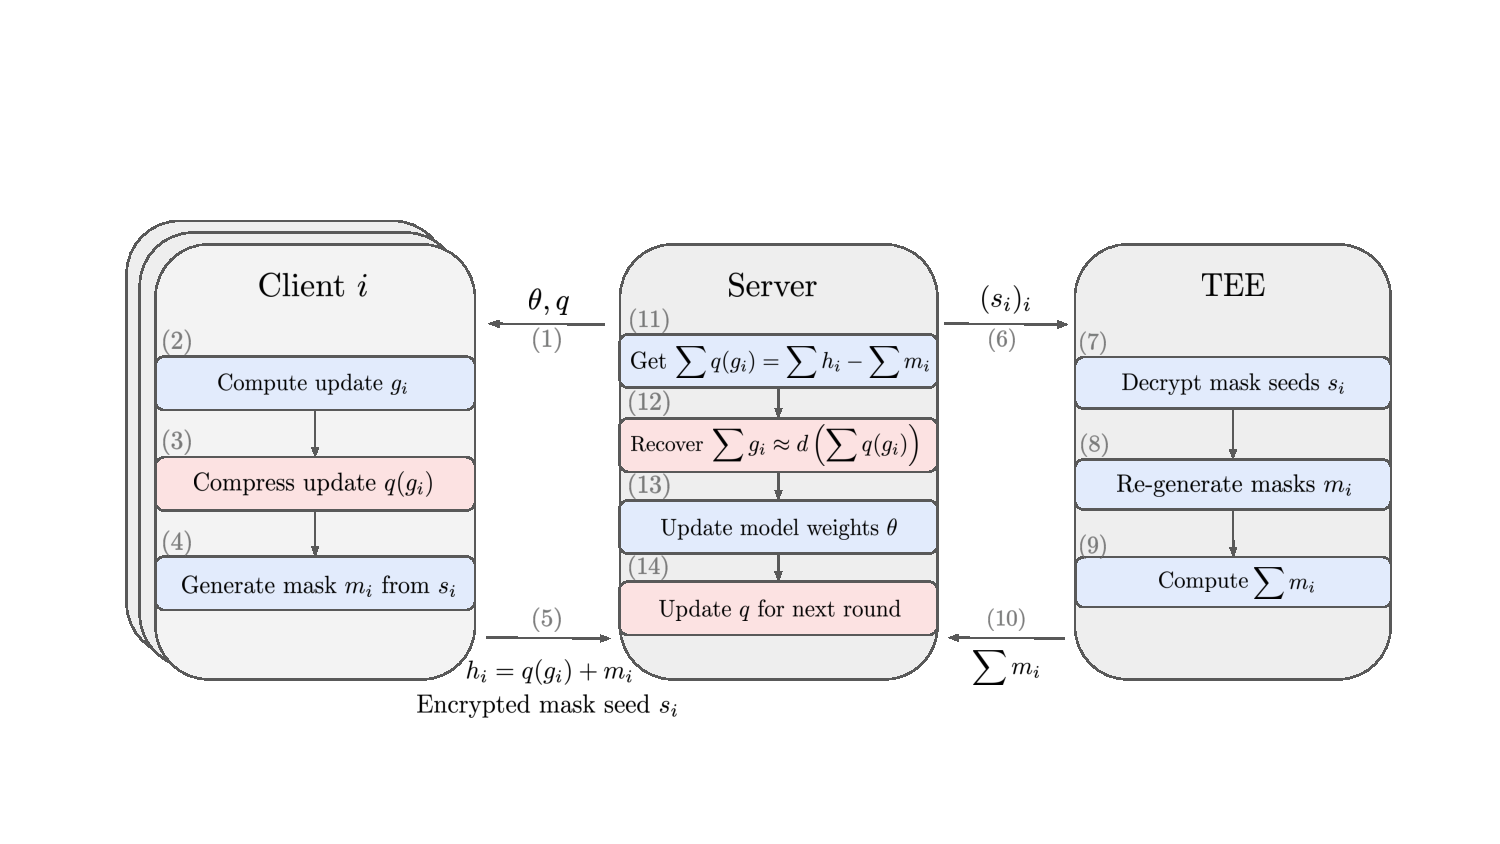
\includegraphics[width=0.8\textwidth]{figs/secagg_summary_new.pdf}
    %\vspace{-5mm}
    \caption{\label{fig:secagg_summary}
    Summary of the proposed approach for one FL round, where we omit the round dependency and \modif{Differential Privacy (DP)} for clarity. Blue boxes denote standard steps and red boxes denote additional steps for uplink compression. Client $i$ computes local model update $g_i$, compresses it with the compression operator $q$, and encrypts it by adding a random mask $m_i$ in the compressed domain, hence reducing the uplink bandwidth (steps 2--4). The server recovers the aggregate in the compressed domain by leveraging any \SecAgg protocol \modif{(steps 7--13, with a TEE-based \SecAgg, see Section~\ref{subsec:secagg})}. Since the decompression operator $d$ is linear, the server can convert the aggregate back to the non-compressed domain, up to compression error (step 12). As with the model weights $\theta$, the compression operator $q$ are also periodically updated and broadcast by the server (step 14). 
    In Section~\ref{sec:method}, we apply the proposed method to scalar quantization and pruning without impacting \SecAgg and propose Secure Indexing, a variant of \SecAgg for extreme uplink compression with product quantization. See Section~\ref{subsec:secagg} for details about \SecAgg and Section~\ref{sec:discussion} for a discussion on~DP.
    }
    \vspace{-3mm}
\end{figure*}



% Our focus in this paper is on 

%Second, scaling cross-device (synchronous) FL to millions of clients with various capabilities and intermittent availability \citep{bonavitz2019federated} suffers from diminishing returns: the wall-clock training time plateaus as the number of clients keeps increasing~\citep{huba2021papaya}. Even though this challenge can be addressed by leveraging the buffered asynchronous aggregation technique proposed by \cite{nguyen2021federated}, compatible with DP and SecAgg, the asynchronous protocol remains bottlenecked by communication latency between the server and the clients.


%Considering the above privacy and scalability goals, we focus on enabling efficient FL communications while keeping a high privacy bar. In addition to the primary objective of speeding up convergence, reducing communication costs brings other significant benefits. Lowering communication requirements addresses selection bias due to undersampling clients with limited connectivity, improving fairness and inclusivity metrics. Better communication efficiency shrinks the carbon footprint of FL, whose fraction attributable to communication can reach 95\%~\citep{qiu2021first}. %Finally, training larger model in FL would be a possibility, when the communication cost is reduced, because local memory or compute requirements can be addressed by modifying the local training loop, for instance with gradient checkpointing \citep{chen2016training}. However, some form of compression would be required to enable efficient communication.


%First, compressing model updates from the client to the server presents several challenges due to compatibility with SecAgg and is an area suitable for further research. 
%Second, upload bandwidth is generally more restricted than download. For instance, according to the most recent FCC report, the ratio of download to upload speeds for DSL/cable providers in the US ranges between 3$\times$ to 20$\times$~\citep{fcc-broadband}. We consider broadband speeds here because devices participate in the FL training while connected to fixed broadband, usually through Wi-Fi~\citep{huba2021papaya}.




% Hence, FL provides the ability to leverage data from massive client populations while ensuring the security and privacy of the client data.
% Go further: compatibility with DP / compression as a mitigation techniques of attacks
% Model and gradient compression intrinsically different.
%  Why not having the secure enclave perform the aggregation?
% \section{Requirements for a Multi-modal Data Science Platform}
\label{sec:requ-holist-data}

In this section we outline the requirements of a multi-modal data science platform and then introduce Vizier as a solution fulfilling these requirements. We start by discussing existing modalities that are widely used to interact with data in data science and their advantages and disadvantages. Converging on a set of modalities we deem to be essential, we then cover several cross-cutting concerns such as reproducibility and dealing with errors that are important no matter what modality is used to interact with data.

%%%%%%%%%%%%%%%%%%%%%%%%%%%%%%%%%%%%%%%%%%%%%%%%%%%%%%%%%%%%%%%%%%%%%%%%%%%%%%%%
\subsection{Modalities for Interacting with Data}
\label{sec:modal-inter-with}

Data scientists often employ several tools during the life-cycle of building a data pipelines. During data discovery, search engines (e.g., open data repositories) and dataset discovery tools (e.g., metadata management tools for data lakes) are used to identify data internal to an organization, data available for purchase, or openly available data that could be used to fulfill the goal the data scientist has in mind. The next step is typically to profile the data and understand its semantics and fitness for the task at hand. At this stage, data visualization is used, either in the form of specialized visualization systems or by employing visualization libraries written in, e.g., Python. This is often done from within notebook environments like Jupyter which can show visualizations inline with the users code. Afterwards, data is curated and integrated. Spreadsheets are often used for manual inspection of smaller datasets, repair of one-off errors, and to calculate basic statistics. Task-specific data cleaning systems or libraries written in a general purpose programming language are employed to (partially) automate this process. The cleaned and integrated data is then used in data analysis (e.g., building and evaluating machine learning models, running analytical queries, \ldots) and the final results of the analysis are visualized. Building a data pipeline is often an iterative process where the user revisits previous steps in the pipeline to deal with errors and to refine the processing.

%%%%%%%%%%%%%%%%%%%%%%%%%%%%%%%%%%%%%%%%%%%%%%%%%%%%%%%%%%%%%%%%%%%%%%%%%%%%%%%%
\subsubsection{Notebooks for Interactive Pipeline Development with Immediate Feedback}
\label{sec:noteb-inter-pipel}
%
Notebook systems like Jupyter and Apache Zeppelin to name just a few have become the quasi-standard for developing data science pipelines. One major advantage of notebooks is their highly interactive nature: users can run pieces of code and immediately observe their results. This makes it easy to debug steps in the pipeline and aids iterative development of pipelines. The outputs recorded in a notebook serve as a documentation of the data preparation and analysis process. Furthermore, most notebook system allow support documentation (typically written in a markup language such as markdown) to be interleaved with code. Even notebook interfaces have become prevalent, most existing implementations are suffer from poor reproducibility, do not support iterative development well, and are not suited well for large and complex pipelines. A recent study~\cite{PM19} on Jupyter notebooks collected from github observed that only 4\% of these notebooks are reproducibly in the sense that they can be rerun without errors and produce the same result as recorded in the notebook. We have argued in \cite{BS20, DG22} that these shortcomings are not inherent to the notebook model, but rather are the result of the architecture of notebook systems which use a long running kernel (e.g., a Python interpreter) and when the user runs a cell in a notebook send the cell's code to the kernel for execution. The kernels state, however, is hidden from the user and except for cell outputs is not encoded in the notebook itself. This leads to unreproducible behavior where the results recorded in the notebook no longer agree with a serial (top-down) execution of the notebook's cells. Furthermore, this can lead to stale results, if the user forgets to rerun cells whose code does dependent on the code in a cell that has been changed. Given the many benefits of and broad use of notebooks, support for a notebook interface is a must for any data science platform. We argue that by providing a notebook interface on top of a specialized workflow engine we can avoid the pitfalls of notebook systems which are thin wrappers around a kernel (Python interpreter). Specifically, we want a solution that supports a notebook interface (\textbf{requirement (N)} which fulfills the following conditions:
\begin{itemize}
\item \textbf{(N1) Serial Execution Semantics:} At any point in time, the results for the cells of the notebook agree with the results produced by a serial execution of the notebook.
\item \textbf{(N2) No Stale Outputs:} The outputs of each cell in the notebook should correctly reflect the current version of the notebook's code.
\item \textbf{(N3) Reproducibility:} The execution of a pipeline (notebook) does not depend on any hidden state. That is, as long as the code in the notebook is deterministic, rerunning a pipeline produces the same output as the original execution.
\end{itemize}

Note that any system that guarantees serial execution of notebooks as defined above, automatically guarantees that there are no stale outputs and that the execution of a notebook is reproducible.


%%%%%%%%%%%%%%%%%%%%%%%%%%%%%%%%%%%%%%%%%%%%%%%%%%%%%%%%%%%%%%%%%%%%%%%%%%%%%%%%
\subsubsection{Spreadsheets for Manual Curation and Exploration}
\label{sec:spre-manu-curat}
%
While notebooks are suited well for programmatic transformation and exploration of data, spreadsheet interfaces enable manual exploration and one-off transformations and fixes~\cite{FG16}. For instance, a user may search for and correct a few mistyped attributes values through a spreadsheet interface. Spreadsheets are also suited well for testing simple data transformations on a few rows using formulas and then once the transformation is satisfactory apply the transformation to a large number of rows by applying the same formula to many rows. Many spreadsheet systems have support for tracking changes made to the spreadsheet, but lack mechanisms to navigate the version history of a spreadsheet and to create branches, e.g., to try out a crazy idea without breaking a deployed version of a data science pipeline. As observed elsewhere~\cite{bendre-19-fhs}, spreadsheet systems do not typically scale to large datasets. While it is anyways infeasible to manually clean and curate large datasets, developing manual fixes on a sample / subset of a large dataset and then deploying the fixes to the dataset can be quite effective. Most spreadsheet systems use a data model that is incompatible with other structured data models such as the relational data model or data frames (which are essentially relations with row indexes) in that (i) columns do not have to be declared but are used by inserting a value into one cell of a column, (ii) the values of a column do not need to belong to a single datatype (e.g., some cells in a column may store strings while others are integers), and (iii) some operations  change the row and column positions rather than their content (e.g., inserting a row, changes the positions of all following rows). To support spreadsheets as a modality (\textbf{requirement (S)}, data science platforms should:
\begin{itemize}
\item \textbf{(S1) Translating between Relations and Spreadsheets:} It should be possible to manipulate standard relations through a spreadsheet view as well as process spreadsheets in other modalities.
\item \textbf{(S2) Supporting Spreadsheet Operations over Relations:} It should be possible to apply spreadsheet operations such as inserting / deleting rows / columns.
\item \textbf{(S3) Scalability:} It should be possible access large datasets through a spreadsheet interface.
\end{itemize}

%%%%%%%%%%%%%%%%%%%%%%%%%%%%%%%%%%%%%%%%%%%%%%%%%%%%%%%%%%%%%%%%%%%%%%%%%%%%%%%%
\subsubsection{Profiling and Interactive Visualizations}
\label{sec:inter-visu}
%
Data profiling and visualization are important tools for data scientists to explore data, understands its semantics, and identify problems with the data.
Data science platforms should support visualizations (\textbf{requirement (V)}). For example, a typical task in the initial data exploration phase of constructing a pipeline is to analyze and visualize the data distributions of columns in a dataset, e.g., by computing histograms for individual columns or by calculating the number of null values per column. Another common approach is to visualize correlations between columns. Both the spreadsheet and notebook modalities discussed so far, do support creation of plots and other data visualizations. Visualization recommendation~\cite{lee-21-l, hu-19-v} guide the user in exploring visualizations that help them to understand their data. A data science platform should support out-of-the-box visualizations  for common tasks (\textbf{requirement (V1)}, e.g., accessing data distributions as histograms as well as provide access to more general visualization tools (\textbf{requirement (V2)} to enable creation of custom visualization of, e.g., analysis results.

%%%%%%%%%%%%%%%%%%%%%%%%%%%%%%%%%%%%%%%%%%%%%%%%%%%%%%%%%%%%%%%%%%%%%%%%%%%%%%%%
\subsubsection{Semi-automated Data Cleaning, Curation, and Integration}
\label{sec:semi-automated-data}
%
As has been observed repeatedly in the past~\cite{nyt:wrangling}, data scientists spend the majority of their time in data discovery, preparation, and curation. Data cleaning, integration, and curation are complex tasks that are time consuming and error-prone. While full automation of these tasks is typically not an option, a plethora of semi-automated tools (e.g., constraint-based data cleaning~\cite{ilyas-15-tcrd}, schema matching~\cite{RB01}, and data integration~\cite{HR06}) which rely on heuristics and often involve the user in curation decisions have been proposed and exist in the form of stand-alone tools and libraries available for languages such as Python. Data science platforms should enable users to use such tools and algorithms in their data science pipelines (\textbf{requirement (C)}. Most approaches for automating data wrangling rely on heuristics to clean data. This is due to the fact that typically insufficient information is available to determine what the correct repair for a dataset is. For instance, when repairing a primary key constraint by tuple deletion~\cite{ilyas-15-tcrd}, one has to retain at most one tuple from each group of tuples with the same primary key value, however, we typically lack information to decide which tuple is the correct one to keep. Thus, data repair algorithms instead use heuristics such as preferring tuples with values that are common in the dataset or optimizing a global metric~\cite{RC17}. Data science platforms should track changes made based on heuristics and how they affect downstream operations as well as provide the user with an overview of what other choices did exist and how different choices would have affected the user's analysis results (\textbf{requirement (U)}):
\begin{itemize}
\item \textbf{(C) (Semi-)automated Data Curation and Integration:} Data science platforms should empower users to access (automated) data curation, cleaning, and integration techniques.
\item \textbf{(U) Tracking the Impact of Uncertain Choices:}  The impact of heuristic choices should be tracked through the operations in a data pipeline to aide the user in understanding how these choices have affected their analysis results and how the results would be affected if another alternative would have been chosen during data cleaning.
\end{itemize}

In summary, all modalities we have discussed so far have in common that they provide ways for the user to interact with data by applying transformations that create new data artifacts or update existing data artifacts and by viewing artifacts through user interfaces. For instance, plotting a histogram of the value distribution of an attribute in a csv file involves several transformations: (i) load the CSV file into a suitable in-memory data structure (e.g., a Pandas dataframe); (ii) aggregate the data to create a histogram; (iii) transform the histogram into a plot. We argue that it is feasible to build multiple modalities as ``views'' on top of a single dataflow platform. This approach has the advantage that the user does not have to to manually transform data between different formats expected by systems implementing the different modalities. Even more important, critical orthogonal functionality  such as versioning (that we will discuss next) has to only be implemented once.

%%%%%%%%%%%%%%%%%%%%%%%%%%%%%%%%%%%%%%%%%%%%%%%%%%%%%%%%%%%%%%%%%%%%%%%%%%%%%%%%
\subsection{Cross-cutting Concerns}
\label{sec:cross-cutt-conc}

Independent of which modality is used to interact with the data, there are important cross-cutting concerns such as reproducibility, supporting the user in iterative development of their data pipelines, dealing with data errors and uncertainty, and how to document data which need to be addressed. Some of the issues with implementing these cross-cutting functionality for specific modalities was already discussing in \Cref{sec:modal-inter-with}, but here we

\begin{itemize}
\item \textbf{(R) Reproducibility and Versioning:} Developing a data science pipeline typically requires several rounds of iterative development and refinement and may involve more than one developer. Keeping track of versions of the pipeline (and the associated results) in a version control manner is critical for aiding users in their development process (e.g., roll back to a past working version of the pipeline or test an experimental idea in a separate branch). However, we argue that unlike in version control systems where the user decides which versions of their code are persisted, for data science platforms it is beneficial if by default all past versions are retained (\textbf{requirement (R1)}). That is there should be no difference between the state kept for supporting undo as well as state kept for versioning. Furthermore, for reproducibility, unless the user's code contains non-deterministic operations, repeated executions of a pipeline should return the same result. Since we want to support interactive modalities like spreadsheets, modifications made through such modalities (e.g., manual edits of cell values or inserting and deleting rows in a spreadsheet) have to be translated into steps in the pipeline (\textbf{requirement (R2)}).
\item \textbf{(I) Supporting Iterative Refinement of Pipelines:} Data pipelines are typically constructed in an iterative fashion by adding additional steps and revisiting prior steps in the pipeline. For example, if an analysis returns unexpected results, the user may backtrack and modify steps in the pipeline which clean the data that is used in the analysis. A data science platform should support users in this process by (i) providing an overview of the structure of the pipeline to help the user to navigate between different parts of the pipeline (\textbf{requirement (O)}), (ii) by providing coarse-grained provenance to help the user identify which steps affected the data used by a pipeline step (\textbf{requirement (P)}), and (iii) ensure that outputs of pipeline steps are always up to date when upstream steps are modified. Note that the last requirement is the ``no stale outputs'' requirement (\textbf{requirement (N2)}) we have already discussed in \Cref{sec:noteb-inter-pipel}.
\item \textbf{(D) Documenting Data and Operations:} One advantage of notebook style interfaces is that they allow code and data to be documented using a markup language. For instance, a user may use this feature to document some insights into the semantics of their data or to explain why they selected a particular cleaning or learning technique. However, documentation in notebooks is associated with steps in the pipeline (cells in the notebook) rather than with pieces of data. While this type of documentation should be support (\textbf{requirement (D1)}), data documentation serves a wide range of purposes such as documenting data semantics (e.g., the year for a column storing dates as a month and day of the month), encoding information of how data was collected and processed, and recording information about issues with the data (e.g., a heart rate measurement is outside of the physically possible range). In \cite{kumari:2021:cidr:datasense} we argued that documentation pertaining to data is mission critical should be associated with the data (\textbf{requirement (D2)}) and should persist through operations (\textbf{requirement (D3)}). For instance, if the user annotated some values in a dataset with a note explaining that these values are suspicious, then aggregated summaries derived from the data should also be associated with these notes.
\item \textbf{(E) Dealing with Errors and Uncertainty:} Uncertainty and errors are prevalent in many application domains due to sensor, outliers~\cite{HA04}, and data entry errors, heuristics applied during data curation, integration~\cite{AS10, FK11b}, and cleaning~\cite{YM15, BS10a}, and misinterpretation of data semantics. Data science platforms should help users in identifying errors, should provide access to semi-automated (heuristic) methods for cleaning and curating data such as the data repair techniques~\cite{B19, ilyas-15-tcrd}. Furthermore, the platform should help the user to determine how choices made during cleaning (whether by a human or an algorithm) affect the results of analyzing the data.
\end{itemize}

In this section we have outlined a set of requirements, both to support specific modalities of interacting with data as well as general requirements that any system for building data science pipelines should support.


%%% Local Variables:
%%% mode: latex
%%% TeX-master: "../2022_IEEE_DEB_Vizier"
%%% End:

%!TEX root=../2022_IEEE_DEB_Vizier.tex

% %%%%%%%%%%%%%%%%%%%%%%%%%%%%%%%%%%%%%%%%
% \begin{figure}[t]
%   \centering
%   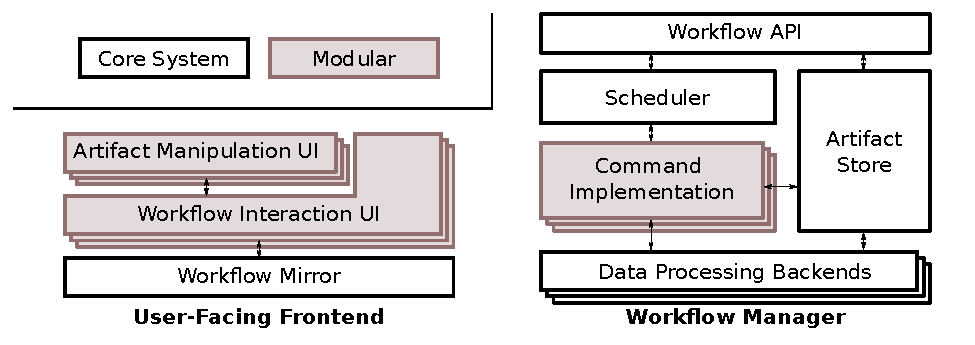
\includegraphics[width=0.7\textwidth]{graphics/systemarch}\\[-5mm]
%   \caption{Vizier's architecture, comprised of a user-facing frontend component and a backend component.}\label{fig:vizier-architecture}
% \end{figure}
% %%%%%%%%%%%%%%%%%%%%%%%%%%%%%%%%%%%%%%%%

%%%%%%%%%%%%%%%%%%%%%%%%%%%%%%%%%%%%%%%%%%%%%%%%%%%%%%%%%%%%%%%%%%%%%%%%%%%%%%%%
\pagebreak[4]
\subsection{Solution Overview}
\label{sec:solution-overview}

%%%%%%%%%%%%%%%%%%%%%%%%%%%%%%%%%%%%%%%%
\begin{wrapfigure}[12]{r}[0pt]{12cm}
  \centering
  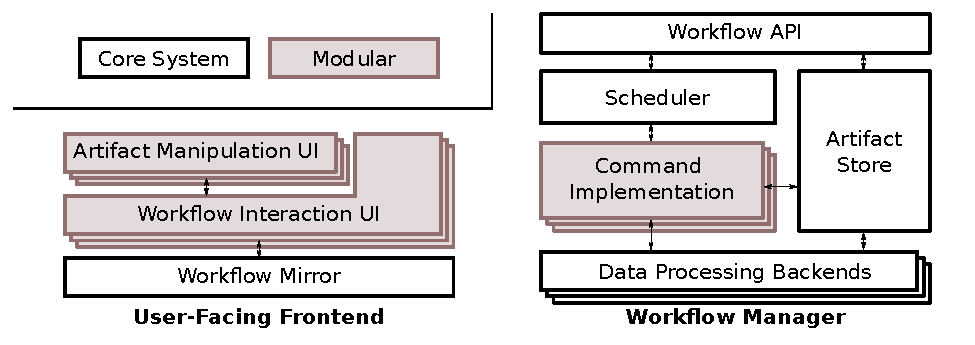
\includegraphics[width=0.7\textwidth]{graphics/systemarch}\\[-5mm]
  \caption{Vizier's architecture, comprised of a user-facing frontend component and a backend component.}\label{fig:vizier-architecture}
\end{wrapfigure}
%%%%%%%%%%%%%%%%%%%%%%%%%%%%%%%%%%%%%%%%
An overview of Vizier's architecture is shown in \Cref{fig:vizier-architecture}.
Addressing requirement \textbf{W1}, the central abstraction in Vizier is a workflow: a linear sequence of steps. % taken by the user in pursuit of a specific objective.
Unlike classical workflow systems, Vizier does not require users to explicitly declare information flow between steps.
Rather Vizier borrows the model employed in popular computational notebooks like Jupyter, where inter-cell communication occurs through a global state (artifacts) passed sequentially through steps.
Following notebook conventions, we refer to these steps as \emph{cells}, and the global state as a \emph{scope}, a map from artifact name to the version of the artifact valid at this point in the workflow. Vizier stores artifacts in common formats through a versioned \textbf{Artifact Store} (\Cref{sec:data-artifacts}), addressing requirement \textbf{A2}.
In \Cref{sec:vizier-workflows}, we formalize Vizier's workflow model, and show how we satisfy requirement \textbf{W3} by instrumenting how each cell interacts with the scope, allowing us to determine what artifact versions are valid.

Vizier's workflow semantics, paired with the versioned artifact store and workflow versioning (\Cref{sec:vizier-history}) addresses requirement \textbf{W2}. % as notebooks have a natural concept of logical order (the order of cells in the notebook) that can be adjusted over time.
% Adding workflow versioning  is sufficient to fully address the requirement.
In contrast, classical notebooks like Jupyter or Zeppelin rely on the global state of an interpreter for inter-cell communication.
Reverting this state to an earlier revision is challenging~\cite{zelnicki:2017:nodebook}, limiting their ability to satisfy requirement \textbf{W3}.
Vizier instead relies on its versioning system, allowing its \textbf{Scheduler} to automatically detect and re-evaluate stale cells (\Cref{sec:vizier-scheduler}).
To address requirement \textbf{A3}, we designed a light-weight uncertain data model that is implemented in Vizier in the form of \textit{caveats}, annotations on data that indicate uncertain values and rows  (\Cref{sec:data-docum-error}).

Addressing requirement \textbf{A1} requires modularity in both Vizier's front- and back-end components.
First, the user's interactions with a workflow and artifacts, whether through a scripting language, graphical interaction, or any other modality, need to be captured for replay (simultaneously addressing requirement \textbf{A4}). In Vizier this is achieved by requiring that every update to an artifact made through a particular modality has to be reflected as an operation in the workflow, i.e., a data update is translated into a workflow update.
Vizier manages a collection of \textbf{Command Implementations} that implement the logic behind these artifact transformations (\Cref{sec:multimodality}).
To streamline the implementation of commands, Vizier's data formats and transformations are built over standard \textbf{Data Processing Backends} like Apache Spark.
% For example, Vizier supports fine-grained provenance over datasets by encoding them as Spark data frames.

The frontend is implemented over a \textbf{Workflow Mirror} that uses websockets to reflect a live view of the workflow the user is editing.
Vizier automatically derives a default \textbf{Artifact Manipulation User Interface} for its notebook interface from each command's parameter schemas. This interface suffices for many templated commands, but the frontend can be further extended to provide a more customized experience, for example for Spreadsheet-style direct manipulation of data (\Cref{sec:spreadsheets}).
As illustrated in \Cref{fig:screenshot}, the frontend displays three \textbf{Workflow Interaction User Interfaces} by default: (i) A direct display of the workflow as a notebook, (ii) a table of contents summary of the notebook, including highlighting from documentation, and (iii) a list of artifacts derived by the notebook.
Several of these components, including the notebook and the artifact list provide access to direct manipulation interfaces.
Additional views currently implemented in Vizier include: (iv) A caveat view (\Cref{sec:data-docum-error}) that shows and tracks potential errors in the workflow and data, (v) a history view that shows the evolution of the workflow over time, and (vi) a data provenance subway diagram view.

%%%%%%%%%%%%%%%%%%%%%%%%%%%%%%%%%%%%%%%%%%%%%%%%%%%%%%%%%%%%%%%%%%%%%%%%%%%%%%%%
\begin{figure}
  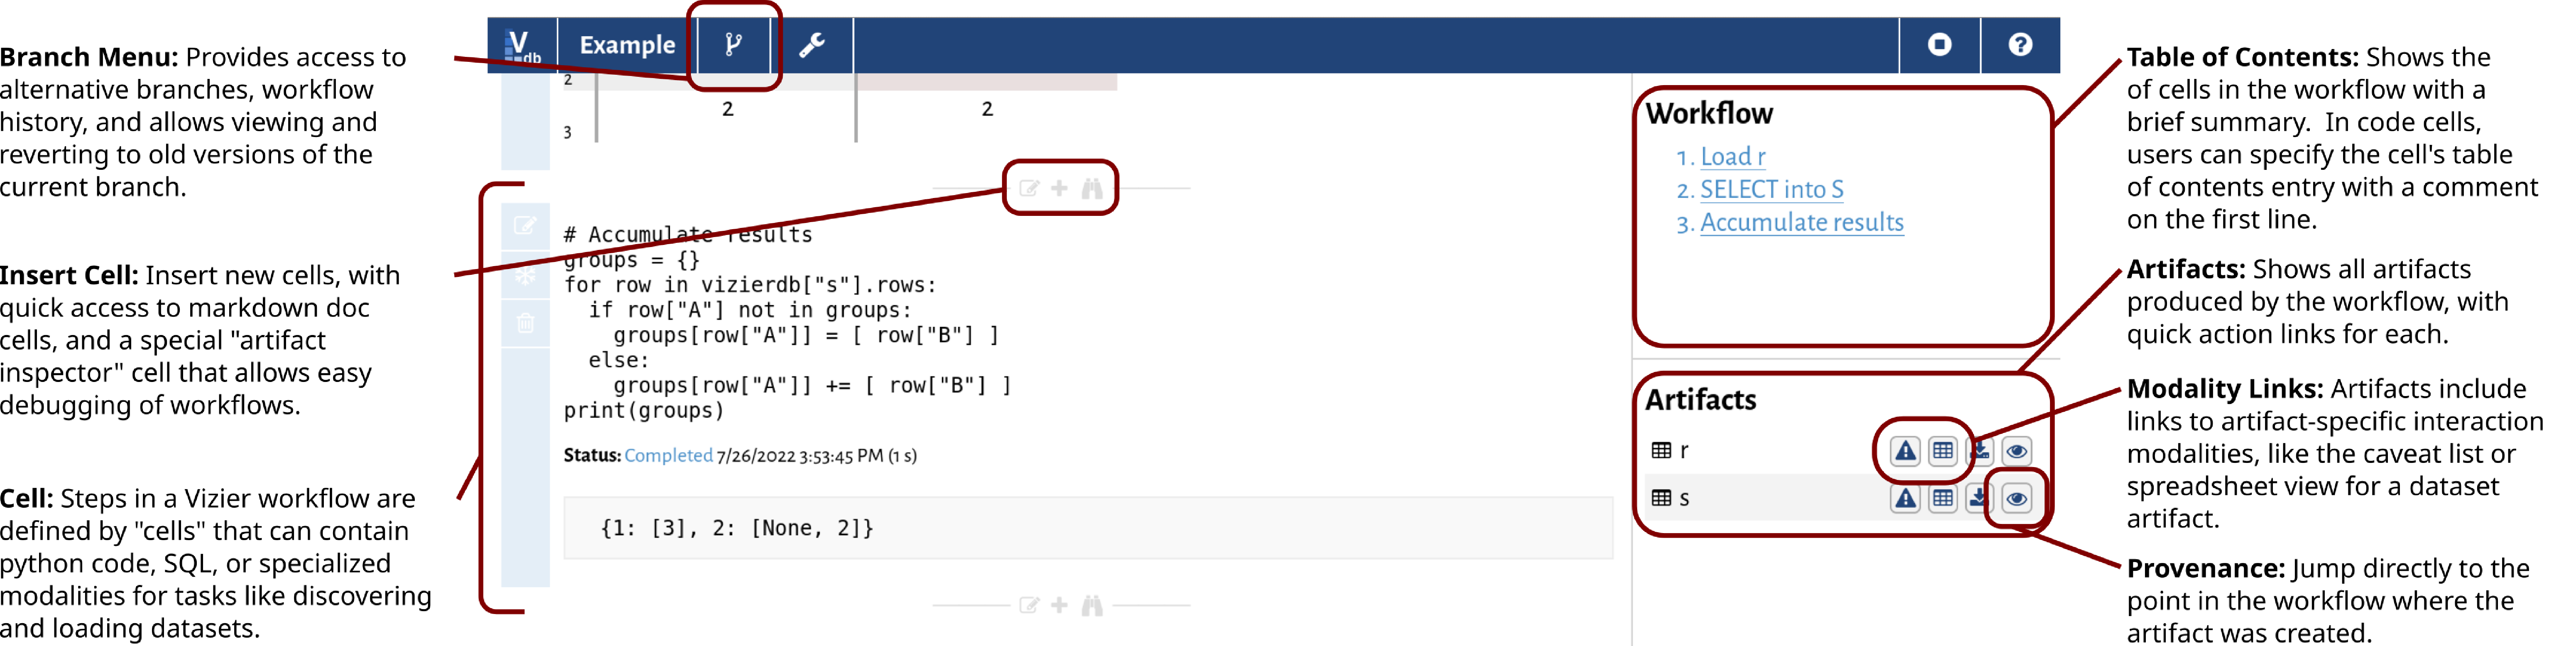
\includegraphics[width=\textwidth]{graphics/screenshot.pdf} 
  \caption{The Vizier User Interface}
  \label{fig:screenshot}
\end{figure}
%%%%%%%%%%%%%%%%%%%%%%%%%%%%%%%%%%%%%%%%%%%%%%%%%%%%%%%%%%%%%%%%%%%%%%%%%%%%%%%%

%%% Local Variables:
%%% mode: latex
%%% TeX-master: "../2022_IEEE_DEB_Vizier"
%%% End:

%!TEX root=../2022_IEEE_DEB_Vizier.tex
%%%%%%%%%%%%%%%%%%%%%%%%%%%%%%%%%%%%%%%%%%%%%%%%%%%%%%%%%%%%%%%%%%%%%%%%%%%%%%%%
\section{Versioned Data Artifact Store}
\label{sec:data-artifacts}

Steps in Vizier workflows create, read, and update \textit{``data artifacts''} or artifacts for short.
To maximize interoperability between cells, Vizier establishes standards for how these artifacts are serialized, which we now discuss. Versions of artifacts are immutable. 
An update to an artifact creates a new object representing the updated artifact. Immutability greatly simplifies handling of state in Vizier and enables us to share artifact versions across multiple revisions of a workflow.

\mypara{Dataset Artifacts}
Tabular data is represented by Vizier as a Spark dataframe~\cite{AX15}, a logical encoding of how a dataset is derived from source data.
The choice to store datasets through a logical representation (specifying the computation instead of its result) is driven largely by the need for managing annotations (requirement \textbf{A3} which is implemented by rewriting the computation to handle annotations), but also results in lower space consumption.
% Because data frames are not serializable, Vizier instead stores dataframe constructors: standardized logic for instantiating a data frame, e.g. by transforming or applying other artifacts.

% Vizier's dataframe constructors are a close analog of SparkML's \texttt{Pipeline}s, which provide a serializable representation of data frame transformation logic.
% Although Vizier provides a pipeline data frame constructor, Pipelines are strictly a representation of transformations, normally requiring glue code to apply the pipeline to an independently loaded dataset;
% Constructors completely capture the logic needed to instantiate a dataframe.

\mypara{Parameter Artifacts}
A parameter artifact can be any primitive value of any data type supported by Apache Spark; We note that this includes simple nested collections like Arrays and Maps.
This type of artifact provides a way to parameterize scripts and other system components, particularly for non-technical users.
% Vizier provides a ``Set Parameter'' command that allows users to specify parameters;
and parameter artifacts are used to pass simple data (e.g., simple constants in Python) between cells.

In addition to these two artifact types, Vizier also supports plots (stored in the vegalite~ \cite{DBLP:journals/tvcg/SatyanarayanMWH17} format), blobs and uninterpreted files, and language-specific constructs, e.g., Python function definitions. For lack of space, we do not further  discuss these other artifact types.

% \mypara{Chart Artifacts}
% Although Vizier provides means for plot generation (e.g., Bokeh, Matplotlib) through messages emitted by a cell, a standardized vegalite~\cite{DBLP:journals/tvcg/SatyanarayanMWH17} artifact format allows multiple cells to collaboratively edit a plot.
% For example, a ``Chart'' command makes it easy for users to quickly visualize a dataset, and then a Spark or Python cell can refine the resulting visualization by tweaking labels, adding markers, or adjusting colors.

% \mypara{Blob and File Artifacts}
% As a fallback to other data formats, Vizier allows cells to export state through a simple blob format.
% For example, Python falls back to encoding global state in `pickle' format, which is stored as a simple blob.
% The blob store is encoded as an in-memory array; If the artifact is large enough to warrant disk IO (e.g., a large model), requires a directory structure (e.g., parquet files), or is otherwise tied to the filesystem, Vizier provide a file artifact format.
% File artifacts are stored in a unique location tied to the artifact identifier.

% \mypara{Function Artifacts}
% Symbols representing language-specific constructs like functions, classes, and imported modules are encoded as raw code.
% Each artifact stores condains code that defines a single symbol under a specific name.
% At time of writing, support for function artifacts requires explicit cross-platform implementation support, although efforts are under way to provide a standardized cross-language interface.




%%% Local Variables:
%%% mode: latex
%%% TeX-master: "../2022_IEEE_DEB_Vizier"
%%% End:

% %!TEX root=../2022_IEEE_DEB_Vizier.tex
\section{Microkernel Notebooks}
As we outline above, a typical computational notebook relies on a kernel, a long-lived interpreter for a scripting language for a scripting language like python that retains the notebook's intermediate state.
When a cell is executed by the user, its contents are evaluated by the long running interpreter; the interpreter's state changes, and any output produced by the cell (e.g., console logs, charts, or maps) is displayed alongside the cell.
This behavior is independent of the order in which the cell appears in the notebook: The user may return to an earlier cell and modify it, but this cell is simply run against the current state of the interpreter.

Although this design allows users to revise cells in the notebook without being forced to re-run all of the notebooks code from scratch, it does pose several problems.
Most notably that it forces users to reason about the internal state of the kernel, for example by manually adopting a single static assignment variable allocation pattern.
Second, it also requires users to manually keep track of how different notebook cells relate to one-another; When a cell is modified, other cells that depend on it may also need revision.
Finally, in this design, persistence (e.g., of the results of a slow-running computation) must be managed entirely by the user.
Moreover, it is up to the user to manually manage this state to ensure consistent versioning, and portability.

One class of systems including Vizier~\cite{BS20,BB19} and Nodebook address these challenges by checkpointing global notebook state in between cell executions and restoring it when a cell is re-executed.
Thus, the cell is always evaluated on the state version emitted by the preceding cell, and changes to the state can be identified so that subsequent cells that depend on modified outputs can be re-evaluated.
This model 


\begin{itemize}
	\item Standard API for interacting with notebook state facilitates multi-modality
	\begin{itemize}
		\item No $N^2$ problem like for jupyter kernels
		\item Not just notebooks
	\end{itemize}
	\item Typed API allows fine-grained provenance
	\begin{itemize}
		\item Reproducibility
		\item Automatic refresh
		\item No hidden (mystical) dependencies
	\end{itemize}
	\item Challenges:
	\begin{itemize}
		\item Communicating state between kernels
		\item 2-dimensional version model (cell-order vs historical-order <- better name for this exists)
		\item Input/output changes in history vs Operation changes in history
		\begin{itemize}
			\item Vizier: Module vs Cell vs Result
			\item The Vizier execution state-model
		\end{itemize}
		\item Scheduling / Deciding state
	\end{itemize}
\end{itemize}

%%% Local Variables:
%%% mode: latex
%%% TeX-master: "../2022_IEEE_DEB_Vizier"
%%% End:

%!TEX root=../2022_IEEE_DEB_Vizier.tex
\section{Workflow Provenance Model and Runtime}
\label{sec:vizier-workflows}

In this section, we outline Vizier's workflow and versioning model, how we determine which cells of a workflow need to be re-executed if a cell is changed, and introduce the parallel scheduler of the system.

% multi-tiered, two-dimensional provenance model.
% We first relate the model to both classical workflow provenance and modern computational notebooks, then discuss how Vizier's model incorporates a temporal dimension, and finally discuss state invalidation and re-evaluation.

\newcommand{\notebook}{\mathcal N}
\newcommand{\workflow}{\mathcal W}
\newcommand{\artifact}{a}
\newcommand{\nbcell}{c}
\newcommand{\outputval}{o}
\newcommand{\readset}{\vec r}
\newcommand{\writeset}{\vec w}
\newcommand{\globalscope}{\mathcal G}
\newcommand{\outputdomain}{\mathcal O}
\newcommand{\valuedomain}{\mathcal D}
\newcommand{\undefinedval}{\bot}
\newcommand{\unknownval}{\circledcirc}
\newcommand{\keyset}{\texttt{keys}}
\newcommand{\changeset}{\Delta}
\newcommand{\variabledomain}{\Sigma}
\newcommand{\diff}[2]{\Delta(#1, #2)}
\newcommand{\evalnb}[1]{\llbracket #1 \rrbracket}

\begin{figure}
  \centering
  \begin{minipage}{0.9\textwidth}
  \begin{lstlisting}[style=pynotebook]
data = read_csv("social_data.csv")
show(data)
  \end{lstlisting}

  \begin{lstlisting}[style=pynotebook]
data["latlon"] = geocode(data["address"])
show(data)
  \end{lstlisting}

  \begin{lstlisting}[style=pynotebook]
censusblocks = read_geojson("blocks.json")
show(censusblocks)
  \end{lstlisting}

  \begin{lstlisting}[style=pynotebook]
data = spatial_join(data, censusblocks, ["latlon", "geometry"])
count_per_block = data.groupby("block_id").count()
show(count_per_block)
  \end{lstlisting}
  \end{minipage}\\[-4mm]
  \caption{A simplified example notebook}
  \label{fig:exampleNotebook}
\end{figure}

%%%%%%%%%%%%%%%%%%%%%%%%%%%%%%%%%%%%%%%%%%%%%%%%%%%%%%%%%%%%%%%%%%%%%%%%%%%%
%%%%%%%%%%%%%%%%%%%%%%%%%%%%%%%%%%%%%%%%%%%%%%%%%%%%%%%%%%%%%%%%%%%%%%%%%%%%
\subsection{Workflow Model}
\label{sec:vizier:eval}

A workflow in Vizier is a sequence of workflow steps (cells) that can read and write artifacts. 
Artifacts are versioned at the granularity of cells. 
A cell writing an artifact $\artifact$ causes a new version of $\artifact$ to be created. 
We will discuss the APIs Vizier exposes to the data interaction modalities for accessing artifacts in \Cref{sec:multimodality}. 
The semantics of a Vizier workflow is the serial execution of the cells of the workflow, where the latest version of each artifact is passed as input to the cell that will be executed next. 
Thus, as long as the cells themselves are deterministic, the artifact versions created by the execution of a workflow are uniquely determined by the workflow itself.

%%%%%%%%%%%%%%%%%%%%%%%%%%%%%%%%%%%%%%%%%%%%%%%%%%%%%%%%%%%%%%%%%%%%%%%%%%%%%%%%
\begin{exam}
  \label{ex:introduction}
  \Cref{fig:exampleNotebook} shows a notebook with a simplified data ingestion, cleaning, and analysis task.
  The notebook loads the dataset (cell 1), geocodes listed street addresses (cell 2), loads a collection of census blocks (cell 3), and computes summary statistics for each census block (cell 4).
  We use this  notebook to illustrate a key challenge of traditional  notebook architectures.
  %
  The user modifies cell 2 to switch to a different geocoder, potentially requiring re-evaluation of the notebook.
  In this specific notebook, the user had the foresight to write in an idempotent style, making it unnecessary to re-run cell 1 to recover the state needed to run cell 2 correctly.
  It is also unnecessary to re-run cell 3, as it does not depend on the output of cell 2.
  However, in traditional notebooks like Jupyter the burden of deciding which cells to re-evaluate rests on the user, creating added overhead and increasing the chance of errors.
\end{exam}
%%%%%%%%%%%%%%%%%%%%%%%%%%%%%%%%%%%%%%%%%%%%%%%%%%%%%%%%%%%%%%%%%%%%%%%%%%%%%%%%

Formally, a Vizier workflow is a sequence $\notebook = \{ \nbcell_1, \ldots, \nbcell_N \}$ of cells. 
The versions of artifacts valid after execution of cell $\nbcell_i$ are modeled as a global scope $\globalscope$ that maps artifact names to artifact versions or the distinguished symbol $\undefinedval$, which indicates that no version of the artifact has been produced yet.  
A cell $\nbcell$ is a function that takes a scope $\globalscope$ as input and produces an updated scope $\globalscope'$: $\nbcell (\globalscope) = \globalscope'$. 
We use $\readset_{\globalscope,i}$ to denote the names of artifacts accessed by cell $\nbcell_i$ applied to $\globalscope_i$. 
The scope parameter is necessary, because a cell may dynamically decide which artifacts to read based on the content of other artifacts.
%
The result $\evalnb{\notebook}$ of  evaluating workflow $\notebook = \{ \nbcell_1, \ldots, \nbcell_N \}$ is defined as the scope $\globalscope_n$ produced by starting with an empty scope $\globalscope_0$ (where all artifact names are mapped to $\undefinedval$), and by computing $\globalscope_{i} = \nbcell_{i}(\globalscope_{i-1})$.








% Cell evaluation in Vizier happens in notebook-order.

% Each cell is (conceptually) evaluated on the scope emitted by the preceding cell.
% Like the workflow systems that inspired it, Vizier retains inter-cell snapshots of scope to preserve notebook-order evaluation semantics while still allowing users to backtrack.


% Denote by $\globalscope$ a global scope that we will formalize shortly;

% We model a cell $\nbcell (\globalscope) = (\globalscope', \readset, \outputval)$ as a deterministic function applied to a global scope that returns a new global scope $\globalscope'$, a read set $\readset$, and an opaque output object $\outputval$ in $\outputdomain$.
% Evaluating the notebook $\evalnb{\notebook} = (\globalscope_N, [\outputval_1, \ldots, \outputval_N)$ produces a final scope $\globalscope_N$ and a sequence of outputs $\outputval_1, \ldots, \outputval_N$ through straightforward composition, starting with an empty scope $\globalscope_0$.
% %  formalized as:
% % $$(\globalscope_i, \readset_i, \outputval_i) = \nbcell_i(\globalscope_{i-1})$$
% % In the above,

%%%%%%%%%%%%%%%%%%%%%%%%%%%%%%%%%%%%%%%%
\begin{wrapfigure}[8]{r}[0pt]{11cm}
  \centering
  \vspace{-4mm}
  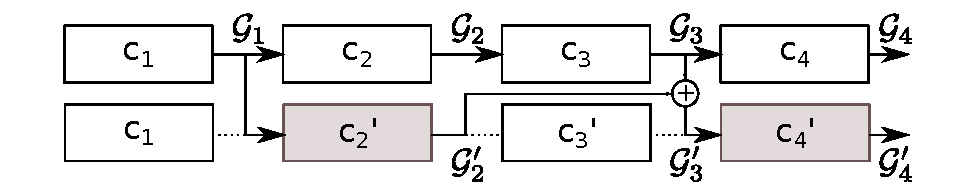
\includegraphics[width=10.5cm]{graphics/eval.pdf}\\[-5mm]
  \caption{Evaluation logic for the example notebook in \Cref{fig:exampleNotebook}.  Edges are labeled with global scope versions.  Cells that are (re-)evaluated are highlighted, dotted lines represent simulated state flow.}
  \label{fig:exampleEval}
\end{wrapfigure}
%%%%%%%%%%%%%%%%%%%%%%%%%%%%%%%%%%%%%%%%
If workflow $\notebook$ is modified by replacing a cell $\nbcell_i$ with a cell $\nbcell_i'$ (denoted as $\notebook[\nbcell_i \backslash \nbcell_i']$), we need to obtain the updated scope $\evalnb{\notebook[\nbcell_i \backslash \nbcell_i']}$. Of course this can be achieved by evaluating $\notebook[\nbcell_i \backslash \nbcell_i']$.
% In lieu of naively re-evaluating the notebook from scratch,
However, to improve performance,  Vizier attempts to update the output of $\evalnb{\notebook}$ by only re-evaluating a subset of the cells.
First, observe that $\globalscope_1, \ldots, \globalscope_{i-1}$ are independent of $\nbcell_i$; and remain unchanged if $\nbcell_i$ is modified.
It is still necessary to have $\globalscope_{i-1}$ to evaluate $\nbcell_i'$; so Vizier caches all intermediate global scopes after evaluating each workflow revision.

% \begin{figure}
%   \centering
%   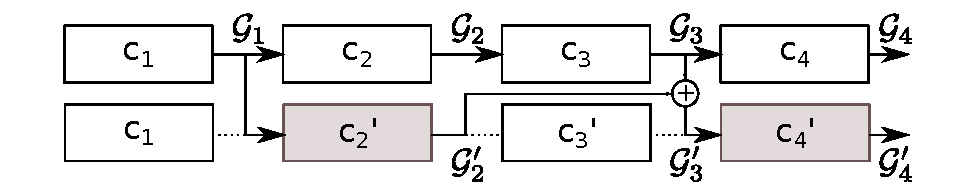
\includegraphics[width=0.7\textwidth]{graphics/eval.pdf}
%   \caption{Evaluation logic for the example notebook in \Cref{fig:exampleNotebook}.  Edges are labeled with global scope versions.  Cells that are (re-)evaluated are highlighted, dotted lines represent simulated state flow.}
%   \label{fig:exampleEval}
% \end{figure}

Naively, we have to still re-evaluate $\nbcell_{i+1}, \ldots, \nbcell_{N}$ using the new scope produced by $\nbcell_i'$. Let us denote the scopes produced by this evaluation as
$\globalscope_{i+1}', \ldots, \globalscope_{n}$.
% $\outputval_{i+1}', \ldots, \outputval_{N}'$.
Vizier uses the readsets $\readset_{\globalscope, i+1}, \ldots, \readset_{\globalscope, N}$, to identify cells $\nbcell_{j}$ for which the same output (artifact versions written by the cell) in $\evalnb{\notebook[\nbcell_i \backslash \nbcell_i']}$ is guaranteed. 
Denote by $\changeset(\globalscope, \globalscope') = \{ k |  \globalscope(k) \neq \globalscope'(k)\}$ the names of artifacts that differ between $\globalscope$ and $\globalscope'$. 
We have to re-execute cell $\nbcell_{i+1}$ if an artifact read by $\nbcell_{i+1}$ has changed, which is the case if $\changeset(\globalscope_i, \globalscope_i') \cap \readset_{\globalscope,i+1} \neq \emptyset$. If $\nbcell_{i+1}$ needs to be re-executed, then we set $\globalscope_{i+1}' = \nbcell_{i+1}(\globalscope_{i}')$. Otherwise, we generate $\globalscope_{i+1}$ by merging the changes made by $\nbcell_{i+1}$ in $\notebook$ to $\globalscope_{i}$ into $\globalscope_{i}'$. That is, for all artifacts $k$ we set
$\globalscope_{i+1}'(k) =   \globalscope_{i+1}(k)$ if $k \in \changeset(\globalscope_i, \globalscope_{i+1})$
and $\globalscope_{i+1}'(k) = \globalscope_{i}'(k)$ otherwise.
% begin{cases}
%   \globalscope_{i+1}(k) &\;\;\;\text{\textbf{if}}\,k \in \changeset(\globalscope_i, \globalscope_{i+1})\\
%   \globalscope_{i}'(k) &\;\;\;\text{\textbf{otherwise}}\\
% \end{cases}$$
 The same approach is applied to decide whether to evaluate or skip the remaining cells in $\notebook[\nbcell_i \backslash {\nbcell_i}']$.


% We formalize a global scope $\globalscope = \{ k_1 \rightarrow v_1, k_2 \rightarrow v_2, \ldots \}$ as a total mapping from an infinite alphabet of variable names $k \in \variabledomain$ to a set of domain values $v \in \valuedomain \cup \{\undefinedval\}$.
% The distinguished symbol $\undefinedval$ denotes an ``undefined'' value, and we assume that finitely many elements of $\variabledomain$ are mapped to non-$\undefinedval$ values (i.e., that $\globalscope$ has finite support).
% Denote by $\keyset(\globalscope) = \{ k | (k \rightarrow v) \in \writeset \wedge v \neq \undefinedval\}$ the keys of the finite support of $\globalscope$.
% Denote by $\changeset(\globalscope, \globalscope') = \{ k |  \globalscope(k) \neq \globalscope'\}$ the change set between $\globalscope$ and $\globalscope'$.

% Given the newly computed $\globalscope_i'$, we want to know if $\nbcell_{i+1}$ needs to be evaluated as well;
% If $\nbcell_{i+1}(\globalscope_i') = (\globalscope_{i+1}', \readset_{i+1}', \outputval_{i+1}')$, we can avoid re-evaluating $\nbcell_{i+1}$ if we can prove that $\outputval_{i+1} = \outputval_{i+1}'$.
% Under the assumption that $\nbcell_{i+1}$ is deterministic with respect to inputs $\readset_{i+1}$, we can guarantee that $\outputval_{i+1} = \outputval_{i+1}'$ when $\readset_{i+1} \cap \changeset(\globalscope_{i}, \globalscope_{i}')$ is empty.
% If we do not need to re-evaluate $\nbcell_{i+1}$, we can reconstruct its output by considering how the original evaluation affected the scope: the write set $\writeset_{i+1} = \changeset(\globalscope_{i}, \globalscope_{i+1})$.
% Concretely $\outputval_{i+1}' = \outputval_{i+1}$, $\readset_{i+1}' = \readset_{i+1}$ and
% $$\globalscope_{i+1}'(k) = \begin{cases}
% \globalscope_{i+1}(k) \textbf{ if } k \in \writeset_{i+1}\\
% \globalscope_{i}'(k) \textbf{ otherwise}
% \end{cases}$$
% \noindent The remaining cells of the notebook are processed in a like manner.

 %%%%%%%%%%%%%%%%%%%%%%%%%%%%%%%%%%%%%%%%%%%%%%%%%%%%%%%%%%%%%%%%%%%%%%%%%%%%%%%%
\begin{exam}
  \Cref{fig:exampleEval} continues the running example from \Cref{ex:introduction}.
  The user has replaced the initial version of cell $\nbcell_2$ with an updated version ${\nbcell_2}'$.
  The global scope produced by preceding cells ($\globalscope_1$) may be re-used unchanged to evaluate ${\nbcell_2}'$, producing scope $\globalscope_2'$.
  $\changeset(\globalscope_2, \globalscope_2')$ is the \lstinline{data} artifact, but the readset of $\nbcell_3$ is empty, and so this cell does not need to be re-evaluated.
  Instead $\globalscope_3'$ is derived by merging variables the cell previously changed (i.e., $\changeset(\globalscope_2, \globalscope_3)$) into the current global scope.
  Finally, Vizier identifies that an element of $\readset_{\globalscope,4}$ (the \lstinline{data} variable) has changed between $\globalscope_3$ and $\globalscope_3'$, necessitating a re-evaluation of cell 4.
\end{exam}
 %%%%%%%%%%%%%%%%%%%%%%%%%%%%%%%%%%%%%%%%%%%%%%%%%%%%%%%%%%%%%%%%%%%%%%%%%%%%%%%%

% \mypara{Frozen Cells}
% Vizier allows users to ``freeze'' cells, temporarily replacing them with no-op commands, but preserving all user-interface elements (including cell outputs), and allowing the cell to be easily re-inserted into the notebook.
% This allows users to quickly disable cells with transient purposes (e.g., sampling cells), or avoid triggering expensive computations while working on an earlier part of the notebook.

% \begin{figure}
%   \centering
%   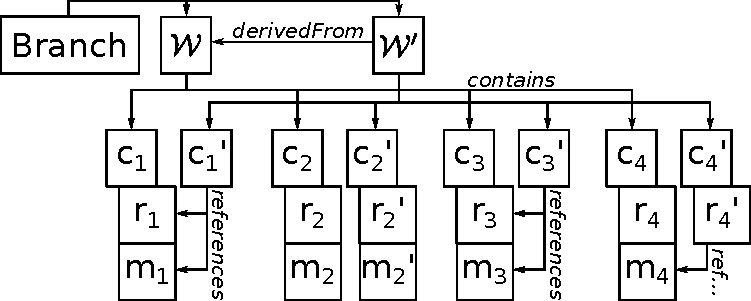
\includegraphics[width=0.45\textwidth]{graphics/history.pdf}\\[-3mm]
%   \caption{History for the running example, assuming cell B was changed as in \Cref{fig:exampleEval}.}
%   \label{fig:exampleHistory}
% \end{figure}

%%%%%%%%%%%%%%%%%%%%%%%%%%%%%%%%%%%%%%%%%%%%%%%%%%%%%%%%%%%%%%%%%%%%%%%%%%%%
%%%%%%%%%%%%%%%%%%%%%%%%%%%%%%%%%%%%%%%%%%%%%%%%%%%%%%%%%%%%%%%%%%%%%%%%%%%%
\subsection{Versioning Workflows}
\label{sec:vizier-history}

%%%%%%%%%%%%%%%%%%%%%%%%%%%%%%%%%%%%%%%%
\begin{wrapfigure}[10]{r}[0pt]{8cm}
  \centering
  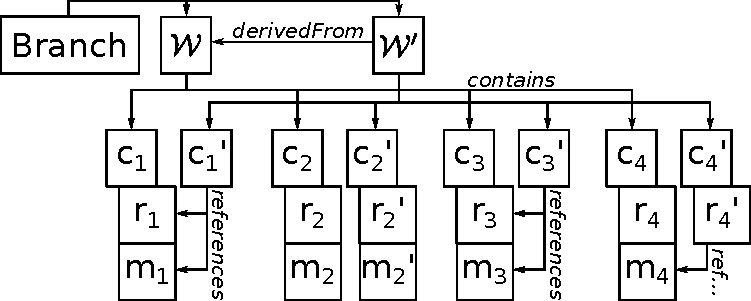
\includegraphics[width=0.45\textwidth]{graphics/history.pdf}\\[-3mm]
  \caption{History for the running example, assuming cell 2 was changed as in \Cref{fig:exampleEval}.}
  \label{fig:exampleHistory}
\end{wrapfigure}
%%%%%%%%%%%%%%%%%%%%%%%%%%%%%%%%%%%%%%%%
Vizier maintains a branching history of the evolution of the notebook.
% We use the term workflow ($\workflow = c_1, \ldots, c_N$) to denote a single state of the notebook.
A cell is further subdivided into (i) \textbf{cell metadata} ($c_i$) that is unique to the workflow (e.g., timestamps and execution status), (ii) \textbf{results} ($r_i$) of executing the cell, and (iii) a \textbf{module} ($m_i$) describing the command executed in the cell.
The latter two components (results and modules) may be shared across workflows.
% In other words, a single cell object acts as a many-to-many-to-many (i.e., 3-ary) relationship between workflow, module, and result entities.
A module object describes the command to be evaluated in a cell.  
This includes its type (e.g., Python or Scala script; SQL query; or one of the graphical widgets), as well as any parameters to the command (e.g., the script itself, or the artifact name to materialize query results as). 
A results object stores references to versions of artifacts in the artifact store created by the execution of the cell. 
We do not materialize the full global scope after each cell, but rather only the changes made to the global scope by the cell (i.e., the cell's write set). 
Any global scope $\globalscope_i$ can be reconstructed from the preceding write sets.

% A results object consists of three items: (i) Messages output by the cell (i.e., $\outputval$), (ii) The cell's readset as a list of name/artifact pairs, and (iii) The cell's writeset as a list of name/artifact pairs.
% Deletion is encoded by writing the distinguished value \texttt{null} to a name.
% As a performance optimization, name/artifact pairs do not embed the artifact literal, but rather a unique artifact identifier.
% This allows for efficient equivalence testing, while avoiding duplication; For example, a ``copy artifact" instruction only needs to clone the artifact identifier under a new name, and not the entire artifact.

% \mypara{Global scope}
% Note that the organizational structure used to persist history information differs from the global scope model used to reason about cell re-use.
% However, the two representations are equivalent.
% Denote by $m_1 \circ m_2$ the right-preferenced composition of \emph{partial} maps $m_1$ and $m_2$ as follows:
% $$m_1 \circ m_2 = \{ k\rightarrow v | (k \rightarrow v) \in m_1 \wedge \not\exists v' \text{ s.t. } (k \rightarrow v') \in m_2 \} \cup m_2$$
% Any global scope $\globalscope_N$ can be recovered by composing the preceding writesets: $\globalscope_N = \globalscope_0 \circ \writeset_1 \circ \ldots \circ \writeset_N$


\begin{exam}
 \Cref{fig:exampleHistory} continues our running example, which in our new terminology is a single branch comprised of two workflows $\workflow_1$ and $\workflow_2$.
  Both notebooks are comprised of four cell objects each.
  Cells 1, 3, and 4 were unchanged between workflows, and so the corresponding cell objects for $\workflow_2$ reference the same module description object as the corresponding cell for $\workflow_1$, while the module descriptions referenced by $\nbcell_2$ and ${\nbcell_2}'$ differ.
  Cells 1 and 3 do not need to be re-evaluated, and so can share their result objects, while Cells 2 and 4 both require re-evaluation and create new result objects.
\end{exam}

%%%%%%%%%%%%%%%%%%%%%%%%%%%%%%%%%%%%%%%%%%%%%%%%%%%%%%%%%%%%%%%%%%%%%%%%%%%%%%%%
\mypara{Workflow and Branch History}
Similar to version control systems like git, each workflow version in Vizier stores a reference to the workflow version it was derived from.
% The difference between workflow versions can be computed by comparing the sequence of modules referenced by the workflow's cells; but simple summary information including the type of change (insert, delete, update) and the affected module (if appropriate) is cached with the workflow object.
A branch is an append-only sequence of workflow versions. % with associated metadata (e.g., a branch name).
The branch contains a reference to the most recent workflow version in the branch. % prior versions are tracked through the series of derived-from references in the workflows themselves.
A new branch may be created from any existing workflow version, including a historical one.

%%%%%%%%%%%%%%%%%%%%%%%%%%%%%%%%%%%%%%%%%%%%%%%%%%%%%%%%%%%%%%%%%%%%%%%%%%%%
%%%%%%%%%%%%%%%%%%%%%%%%%%%%%%%%%%%%%%%%%%%%%%%%%%%%%%%%%%%%%%%%%%%%%%%%%%%%
\subsection{Parallel Scheduler}\label{sec:vizier-scheduler}

The evaluation model presented in \Cref{sec:vizier:eval} relies exclusively on \textit{dynamic provenance}, where Vizier is informed about the readset and writeset of a cell at runtime when the cell accesses artifacts through Vizier's API.
% that assist in determining whether a cell needs to be re-evaluated.
However, dynamic provenance is not always sufficient.
For example, Vizier evaluates cells in parallel where possible, but dynamic provenance is not available until the cell has already been evaluated.
Static provenance, which can derive a cell's read and write sets through static dataflow analysis of its source code, can be computed upfront.
However, static dataflow analysis is of necessity an approximation for some cell types; language features like control flow and dynamic code evaluation can lead to over- (or under-) estimates of the cell's read and write sets. % , especially with respect to a specific global scope.
Vizier uses a novel approach which refines static provenance at runtime using dynamic provenance~\cite{DG22}.

Fundamentally, Vizier's scheduler needs to assign each cell in a running workflow to one of four lifecycle stages: (i) \textbf{DONE} when the cell has a valid result object, (ii) \textbf{PENDING} when the cell depends (directly or transitively) on a cell that does not have a result object, and (iii) \textbf{RUNNING} when the cell's dependencies have a valid result object but the cell itself does not.
We further distinguish as (iv) \textbf{STALE} those cells in the \textbf{PENDING} stage for which we can conclusively determine that re-evaluation is required.
% Lifecycle stage transitions are monotonic.

To manage lifecycle transitions, Vizier's scheduler relies on a combination of static and dynamic provenance~\cite{DG22}.
It uses static provenance to generate an over-approximation on the read and write dependencies of a cell\footnote{As we argue in~\cite{DG22}, to deal with languages that support dynamic code evaluation such as Python, it would be necessary to allow under-approximations of read and write sets (missed data dependencies) and compensate for them at runtime. However, this not implemented in Vizier yet; attempts to dynamically read variables not in the maximal readset are flagged as errors.}.
  % Vizier does not presently support purely dynamic dependencies through e.g., dynamic code evaluation.  A read or write access on a variable not discovered through static analysis triggers an execution error.}.
Accordingly, the scheduler tracks an over-approximation of the read and writesets at each step of the workflow, and refines them when the execution of cell finishes and we know its precise read and write set. 
This approximation is used by Vizier's scheduler to omit cells from re-execution or schedule them for parallel execution if we can determine that it is safe to do so based on these over-approximations.

% Approximate global scopes generalize our prior definition of a global scope by extending the value domain to include the value $\unknownval$, denoting an unresolved value (i.e. variables in an approximate global scope are drawn from $\valuedomain \cup \{\undefinedval, \unknownval\}$).
% Like a regular global scope, an approximate global scope is derived by concatenating writesets ($\globalscope_i = \globalscope_{i-1} \circ \writeset_i$).
% However, if the cell is in a lifecycle stage other than \textbf{DONE}, its previous writeset is not valid.
% Instead, Vizier uses static analysis to derive an upper bound on the writeset $\writeset_{\max} \subseteq \variabledomain$, the maximal set of variables that the cell is allowed to write to.
% When the cell's writeset is not (or may not be) valid, the approximate global scope is instead updated by making each element of $\writeset_{\max}$ an unknown:
% $\globalscope_{i} = \globalscope_{i-1} \circ \{ k \rightarrow \unknownval | k \in \writeset_{\max, i} \}$

% \Cref{alg:lifecycleStage} explains how Vizier derives the lifecycle stage of a cell from the global scope emitted by the preceding cell, the cell's readset (if it exists), and the bound on the readset derived from static analysis.
% The first consideration is whether the cell's prior result object is still valid.
% If there is no prior result object (e.g., because the cell is newly inserted), or if the prior result object is definitely invalid (i.e., because a previously read value was definitely overwritten by a re-evaluated cell), the cell must be re-evaluated.
% What remains is whether the cell can be immediately evaluated (all variables in the upper bound on the readset are defined), or not.

% \begin{algorithm}
% \caption{\lstinline{lifecycle_stage}($\globalscope$, $\readset$, $\readset_{\max}$)}
% \label{alg:lifecycleStage}
% \begin{algorithmic}
%   \REQUIRE{$\globalscope$: The approximate global scope from the prior cell.}
%   \REQUIRE{$\readset$: Either a partial map from $\variabledomain$ to $\valuedomain$ denoting the actual read set if one exists, or $\unknownval$ if the cell is new.}
%   \REQUIRE{$\readset_{\max}$: A set over $\variabledomain$, denoting the statically derived upper bound on the cell's read set.}
%   \ENSURE{$\ell$: The current lifecycle stage of the cell.}
%   \IF{$\readset = \unknownval$ or there exists a $(k \rightarrow v) \in \readset$ such that $\globalscope(k) \neq \unknownval$ and $\globalscope(k) \neq v$}
%     \IF{there exists a $k \in \readset_{\max}$ such that $\globalscope(k) = \unknownval$}
%       \STATE $\ell = \textbf{STALE}$
%         \COMMENT{The cell needs to be re-evaluated, but is missing a dependency}
%     \ELSE
%       \STATE $\ell = \textbf{RUNNING}$
%         \COMMENT{The cell needs to be re-evaluated, and is ready to run}

%     \ENDIF
%   \ELSIF{there exists a $(k \rightarrow v) \in \readset$ where $\globalscope(k) = \unknownval$}
%     \STATE $\ell = \textbf{PENDING}$
%       \COMMENT{The cell may not need re-evaluation, but we don't know yet.}
%   \ELSE
%     \STATE $\ell = \textbf{DONE}$
%       \COMMENT{We can guarantee that the cell does not need re-evaluation.}
%   \ENDIF
% \end{algorithmic}
% \end{algorithm}

% When a cell transitions into the \textbf{RUNNING} state, the scheduler starts the corresponding cell.
% When the cell finishes, it has a state that matches the preceding global state, and transitions into the \textbf{DONE} state.

%%% Local Variables:
%%% mode: latex
%%% TeX-master: "../2022_IEEE_DEB_Vizier"
%%% End:
% %!TEX root=../2022_IEEE_DEB_Vizier.tex
\section{Microkernel Notebooks}
As we outline above, a typical computational notebook relies on a kernel, a long-lived interpreter for a scripting language for a scripting language like python that retains the notebook's intermediate state.
When a cell is executed by the user, its contents are evaluated by the long running interpreter; the interpreter's state changes, and any output produced by the cell (e.g., console logs, charts, or maps) is displayed alongside the cell.
This behavior is independent of the order in which the cell appears in the notebook: The user may return to an earlier cell and modify it, but this cell is simply run against the current state of the interpreter.

Although this design allows users to revise cells in the notebook without being forced to re-run all of the notebooks code from scratch, it does pose several problems.
Most notably that it forces users to reason about the internal state of the kernel, for example by manually adopting a single static assignment variable allocation pattern.
Second, it also requires users to manually keep track of how different notebook cells relate to one-another; When a cell is modified, other cells that depend on it may also need revision.
Finally, in this design, persistence (e.g., of the results of a slow-running computation) must be managed entirely by the user.
Moreover, it is up to the user to manually manage this state to ensure consistent versioning, and portability.

One class of systems including Vizier~\cite{BS20,BB19} and Nodebook address these challenges by checkpointing global notebook state in between cell executions and restoring it when a cell is re-executed.
Thus, the cell is always evaluated on the state version emitted by the preceding cell, and changes to the state can be identified so that subsequent cells that depend on modified outputs can be re-evaluated.
This model 


\begin{itemize}
	\item Standard API for interacting with notebook state facilitates multi-modality
	\begin{itemize}
		\item No $N^2$ problem like for jupyter kernels
		\item Not just notebooks
	\end{itemize}
	\item Typed API allows fine-grained provenance
	\begin{itemize}
		\item Reproducibility
		\item Automatic refresh
		\item No hidden (mystical) dependencies
	\end{itemize}
	\item Challenges:
	\begin{itemize}
		\item Communicating state between kernels
		\item 2-dimensional version model (cell-order vs historical-order <- better name for this exists)
		\item Input/output changes in history vs Operation changes in history
		\begin{itemize}
			\item Vizier: Module vs Cell vs Result
			\item The Vizier execution state-model
		\end{itemize}
		\item Scheduling / Deciding state
	\end{itemize}
\end{itemize}

%%% Local Variables:
%%% mode: latex
%%% TeX-master: "../2022_IEEE_DEB_Vizier"
%%% End:

%!TEX root=../2022_IEEE_DEB_Vizier.tex

\section{Multimodality}
\label{sec:multimodality}

As noted in \Cref{sec:vizier-history}, cells in Vizier implement a variety of different modalities, including scripting languages (e.g., Python, Scala), query languages (e.g., SQL), as well as graphical widgets for data ingestion, transformation, and curation (e.g., Load Dataset, Pivot Table, Repair Key).
We refer to the evaluation logic for each modality as \emph{cell command}.
Each cell in a Vizier workflow identifies the command that should run to evaluate the cell, along with a set of arguments to that command.
For example, the SQL cell (\texttt{sql.query}) takes two arguments: the text of a SQL query, and an optional name to materialize the result table as. In this section, we discuss how these modalities are implemented as cell types in Vizier. % and how they are presented in Vizier's notebook view.

A command is defined by the following methods:
(i) \textbf{schema}: Returns a schema for the arguments the command accepts;
(ii) \textbf{summary(arguments)}: Returns a textual description of the behavior of the command when parameterized by the provided arguments;
(iii) \textbf{dependencies(arguments)}: Returns the over-approximation of the set of names of artifacts read (resp., written) by the cell as parameterized by the provided arguments, or indicates that either or both bounds can not be computed; and
(iv) \textbf{evaluate(arguments, context)}: Evaluates the cell on the command, parameterized by the provided arguments and a context object.

The context object on which commands are evaluated provides a read/write interface to the global scope and a way to emit messages to be displayed alongside the cell in the notebook view.
As we discuss in \Cref{sec:vizier-workflows}, the global scope maps artifact names to artifact versions.
Artifacts are not persisted directly as part of the global scope, but rather are references to our write-only artifact store.\footnote{As mentioned before, artifact versions are immutable in Vizier which simplifies version management. We leave optimizations that selectively violate this policy and update artifacts or store deltas instead of creating full updated versions of artifacts to future work.}
When a cell implementation writes an artifact through the context, the artifact version is serialized and written into the artifact store.
The artifact store assigns the artifact (version) a unique identifier, which is then saved into the scope.
Similarly, to read an artifact, a cell implementation first reads the artifact identifier out of the scope, and then accesses the corresponding artifact version from the store.


%\subsection{Language APIs}
% \mypara{Language APIs}
Cells implementing runtimes for general-purpose languages need to provide users of those languages with a way to interact with the global notebook state.
This entails (i) providing a mechanism to reference the scope and import artifacts within a language-specific format, and (ii) predicting how the user-provided code will interact with the state to bound provenance.

\mypara{Python}
%
Python cells are evaluated in an independent interpreter to avoid concurrency bottlenecks from the global interpreter lock (GIL).
Thus, a key challenge is minimizing the volume of state transferred into and out of each interpreter.
Global scope is lazily loaded by populating the global state with a set of proxy objects, one for each artifact in the scope. % We discuss this based on the example of Python and SQL cells.
%
% When a variable is accessed, the proxy object is ``hydrated'' from the artifact store; From that point on, the proxy object routes all function invocations, property accesses, and operator overload invocations to the hydrated artifact.
% Several small values, including primitive constants and module references, are not compatible with proxy objects, but are small enough to allow them to be hydrated in all cells with negiligible performance cost.
%
Access to the Vizier context for messaging and artifact access occurs through a control bus that, by default, operates over the python process' standard input and output streams.
% Python's normal standard output and error streams are overridden and any output over these channels is converted into control messages; Standard input is disabled for the user-provided script.
Vizier defines a special `show' command within the module to produce structured messages (analogous to placing an item on the last line of a Jupyter cell).
The show command includes support for most Vizier-defined types, matplotlib and bokeh plots, and provides fallbacks using the Jupyter-standard \texttt{\_repr\_html\_} method, or direct stringification as a final resort.
% Vizier also discourages direct file IO by overriding the \texttt{open} command to print a warning message.
%
For predictive dependency tracking, and to identify variables that are modified, Vizier relies on Python's \texttt{ast} module, which provides an introspective compilation and code analysis framework.
Vizier performs lightweight dependency analysis~\cite{DG22} to bound the cell's read and write dependencies.

% identify variables accessed or modified by the cell's code.
% This analysis is used both to bound the read and write dependencies, as well as to determine which variables are exported into the global scope at the end of the cell.
% The AST module is also used to extract code for exported function, module, and class symbols.

\mypara{SQL}
%
SQL cells are parsed and evaluated by Apache Spark.
% Spark provides a convenient global catalog, allowing access to named functions, tables, and other values.
% However, because the specific assignment of names to values varies depending on position in the notebook, relying on the global catalog is not thread-safe.
% Instead,
Vizier intercepts the parsed SQL query AST and manually injects references to the corresponding artifacts --- either datasets or python functions --- where needed.
Spark-provided view name decorators make it possible for the injected views to retain their names from the query, avoiding incomprehensible error messages.
The same injection logic is also used to statically identify exact read and write dependencies.

% Spark has native support for Python User-Defined Functions, but this support is geared towards users accessing spark through its python frontend (\texttt{pyspark}).
% Crucially, it relies on a customized serialization format (\texttt{cloud-pickle}) that is not portable across versions of the serialization library or python.
% When Vizier identifies a reference to a python-defined UDF in a SQL query, it spins up a python interpreter, serializes the UDF, and caches it for subsequent use.

% \mypara{Scala}
% Scala cells are run directly within the Vizier JVM through the Scala reflection toolbox.
% % This feature of Scala allows scala code to be compiled and evaluated at runtime; including support for access to global state.
% % The evaluated code does not have access to local variables; Vizier works around this by passing state in through a thread-local global variable.
% % Like Python cells, Vizier overrides the \texttt{print} and \texttt{println} methods to produce messages rather than standard out.
% At present, access to global state in a scala cell occurs manually; A \texttt{vizierdb} object is created to allow cells to interact with the global scope, or to display more elaborate messages than text allows.
% Similarly, at time of writing, dependency analysis is not yet supported.


%%% Local Variables:
%%% mode: latex
%%% TeX-master: "../2022_IEEE_DEB_Vizier"
%%% End:

% 
\section{The Notebook Modality}\label{sec:notebook-modality}



%%% Local Variables:
%%% mode: latex
%%% TeX-master: "../2022_IEEE_DEB_Vizier"
%%% End:

%!TEX root=../2022_IEEE_DEB_Vizier.tex
\section{Interactive Spreadsheets}
\label{sec:spreadsheets}

A key feature of Vizier is support for direct interaction with artifacts~\cite{BS20}, most notably a spreadsheet-like interface for interacting with Spark Data Frames.
Spreadsheets provide a data exploration experience that is distinct from notebooks.
Users are limited to a single dataset, but have significantly more flexibility when exploring the data.
For example, it is common on small datasets (e.g., under 1000 rows) for users to complete preliminary data cleaning tasks like outlier detection, data integration, repair of typos and outliers, and even some limited computation (e.g., deriving new fields) in a spreadsheet prior to working with the data further (e.g., in a notebook).
Another common use case is manual data entry; The user may enter the entire dataset, or may generate a data entry template (e.g., with a script) and import the resulting file into another tool.

% In both cases, the relationship to the original dataset, and any consequent provenance information is lost.
Vizier's spreadsheet interface is intended to provide a view over a subset of the notebook, allowing users to interact with the dataset in the appropriate modality, while simultaneously preserving workflow provenance  through interactions.
% Furthermore, our goal is to present the spreadsheet as a View over a subset of the notebook.
As the user interacts with the spreadsheet, their edits are reflected in the notebook as new cells.
As the user edits the notebook, their edits are likewise reflected in the spreadsheet --- If the source data frame is updated in the notebook, Vizier attempts to re-apply the user's edits to the updated data.

\mypara{Track Changes as a View}
%
To support bi-directional interaction between spreadsheet and notebook views, Vizier implements a series of specialized cell types that mimic SQL DDL and DML operations, allowing for inserting, deleting, or reordering columns and rows, or for updating individual cell values.
We refer to the operations described by these cell types collectively as the Vizual language~\cite{FG16,BS20}.

Vizual is based on the principle that the user's interactions with a database  can be modeled as views over an original version of the data.
As prior work has shown, a view defined over a table can mimic the effects of any DDL~\cite{DBLP:journals/pvldb/CurinoMZ08} or DML~\cite{DBLP:journals/pvldb/NiuALFZGKLG17} operation applied to the table.
Analogously, each Vizual cell in the notebook uses Spark's standard data frame manipulation language to apply a successive transformation to the dataset that mimics the user's interaction.
To ensure that the spreadsheet remains responsive, a shim layer tentatively injects predicted updates to the user's interactions until the effects of the user's edit are fully applied~(e.g., as \cite{DBLP:conf/icde/GuptaDGUW09}).

In SQL DML, update operations specify target rows by a predicate.
By contrast, operations in a spreadsheet explicitly target specific rows of data, requiring Vizier to assign unique identifiers to each record to encode their order in the spreadsheet\footnote{We assume that the number of columns will remain manageable and reference them purely by name}.
To allow Vizual operations to be replayed as source data changes, these identifiers should remain stable through data transformations.
For derived data, Vizier uses a row identity model similar to GProM's~\cite{DBLP:journals/debu/ArabFGLNZ17} encoding of provenance.
Derived rows, such as those produced by declaratively specified table updates, are identified by an appropriate combination of input tuple identifiers. For example, rows in the output of a join are identified by combining identifiers from the source rows that produced them into a single identifier, and rows in the output of a projection or selection use the identifier of the source row that produced them.
% as follows:
% (i) Rows in the output of a projection or selection use the identifier of the source row that produced them;
% (ii) Rows in the output of a \texttt{UNION ALL} are identified by merging the identifier of the source row with an identifier marking which side of the union the row came from (note that this change renders the \texttt{UNION} operator non-commutative).
% (iii) Rows in the output of a cross product or join are identified by combining identifiers from the source rows that produced them into a single identifier; and (iv) Rows in the output of an aggregate are identified by each row's group-by attribute values.

The remaining challenge is assigning row identifiers to source data, which we want to remain stable through changes to the source data so that spreadsheet operations can be replayed.
Ideally, the data would include a unique identifier that we can leverage; but this is not always the case.
Storing the data in a revision control system~\cite{DBLP:conf/cidr/BhardwajBCDEMP15,DBLP:journals/pvldb/HuangXLEP17}, is not always a viable option~\cite{DBLP:conf/sigmod/AlagiannisBBIA12}.
A more heavyweight approach is to link records across revisions of a dataset~\cite{DBLP:conf/sigmod/YilmazWXNEP18}, but this adds non-negligible overhead to common-case data revisions.
Vizier presently supports persistent identifiers through append- or edit-only revisions by assigning each record a unique identifier based on its position, and a hash of its contents.
This approach has the benefit of being lightweight (it can be applied in a single pass), and resilient.
In contrast to simply using a hash-based identifier, the approach supports duplicate records.
Conversely, solely using a position-based identifier could lead to spreadsheet operations being applied to the wrong row in case of insertions.
%
While techniques for creating identifiers that are stable under updates has been studied extensively for XML databases (e.g., ORDPATH~\cite{DBLP:conf/sigmod/ONeilOPCSW04}) and recently also for spreadsheet views of relational databases~\cite{DBLP:journals/pvldb/BendreSZZCP15}, the main challenge we face in Vizier is how to retain row identity when a new version of a dataset is loaded into Vizier, as opposed to keeping identity consistent once the data is already in the system.
% In this scenario we only have access to two (identifier-free) snapshots of the dataset and no further information on how they relate to each other.

%% Local Variables:
%%% mode: latex
%%% TeX-master: "../2022_IEEE_DEB_Vizier"
%%% End:

%!TEX root=../2022_IEEE_DEB_Vizier.tex

%%%%%%%%%%%%%%%%%%%%%%%%%%%%%%%%%%%%%%%%%%%%%%%%%%%%%%%%%%%%%%%%%%%%%%%%%%%%%%%%
\section{Data Documentation, Error, and Uncertainty Management with Caveats}
\label{sec:data-docum-error}

Like notebook systems, Vizier enables users to document their workflow through markdown cells which do not manipulate artifacts, but simply serve as documentation. 
However, some documentation is specific to individual artifacts, or their component parts (e.g., rows, or columns); 
We would like such documentation to accompany the data as it is transformed~\cite{kumari:2021:cidr:datasense}.
Like other annotation management systems including Mondrian~\cite{GK05} and DBNotes~\cite{bhagwat-05-anmsrd},
Vizier empowers users to annotate data with textual comments. 
However, in contrast to these systems, in Vizier these annotations also have a precise semantics: they encode uncertainty about an attribute value of a row or the existence of a row. 
This is important, because uncertainty arises naturally in most data science pipelines (e.g., because of errors in the data or because of heuristic choices during data cleaning) and if data analysis ignores the uncertainty in the data, it can lead to analysis results that cannot be trusted.
To address this issue, caveats are propagated through operations on dataset artifacts in Vizier using an efficient uncertain query semantics we have developed~\cite{FH19, FH21}. 
Thus, caveats on values and rows in the result of an analysis conducted using Vizier encode information about how data cleaning and curation operations on the data used in the analysis affect the analysis result. 
Furthermore, Vizier's implementation of data cleaning operations introduce caveats to encode information about other possible repairs.

%%%%%%%%%%%%%%%%%%%%%%%%%%%%%%%%%%%%%%%%%%%%%%%%%%%%%%%%%%%%%%%%%%%%%%%%%%%%%%%%
\subsection{Incomplete Databases}
\label{sec:incomplete-databases}

Formally, caveats in Vizier are based on an approximation of incomplete databases. An incomplete database $\pdb = \{D_1, \ldots, D_n\}$ is a set of deterministic databases called possible worlds that encode alternative possibilities for the state of the real world: one possible world corresponds to the actual state of the real world, but we do not know which. 
As an example, consider an analyst that has to find the names of important customers (e.g., who ordered products totaling more than \$500). 
An example instance is shown in \Cref{fig:example-customer-database}. 
A common method for primary key repair is to group rows by their PK values and select one row from each group to be retained. 
However, typically we have insufficient information to know which row is the correct choice and will have to rely on heuristics (e.g., selecting the most recently updated row if this information is available). 
Incomplete databases can be used to model this uncertainty: we create an incomplete database whose worlds are all the repairs of the database violating the constraint~\cite{DBLP:journals/vldb/BeskalesIGG14}.
\Cref{fig:example-customer-database} shows two (out of 4) possible repairs for this dataset.

%%%%%%%%%%%%%%%%%%%%%%%%%%%%%%%%%%%%%%%%
\begin{figure}[t]
  \centering

  \begin{minipage}[b]{0.31\linewidth}
\centering
    \textbf{Customer Relation}\\[3mm]
    %%%%%%%%%%%%%%%%%%%%%%%%%%%%%%%%%%%%%%%%
    \begin{tabular}{c|c|c}
      \thead{cid} & \thead{name} & \thead{total} \\     \hline
      1         & Peter          Petersen        & 1000 \\
      1         & Peter          Petersen        & 950  \\
      2         & Bob            Smith           & 300  \\
      3         & Alice          Smith           & 400  \\
      3         & Alice          Smith           & 600  \\
    \end{tabular}
    %%%%%%%%%%%%%%%%%%%%%%%%%%%%%%%%%%%%%%%%
  \end{minipage}
%
  \begin{minipage}[b]{0.31\linewidth}
\centering
    \textbf{Possible       World           (Repair) $D_1$}\\[3mm]
    %%%%%%%%%%%%%%%%%%%%%%%%%%%%%%%%%%%%%%%
    \begin{tabular}{c|c|c}
      \thead{cid} & \thead{name} & \thead{total} \\       \hline
      1         & Peter          Petersen        & 1000   \\
      2         & Bob            Smith           & 300    \\
      3         & Alice          Smith           & 400    \\
    \end{tabular}
    %%%%%%%%%%%%%%%%%%%%%%%%%%%%%%%%%%%%%%%%
  \end{minipage}
%
  \begin{minipage}[b]{0.31\linewidth}
\centering
    \textbf{Possible       World           (Repqir) $D_2$}\\[3mm]
    %%%%%%%%%%%%%%%%%%%%%%%%%%%%%%%%%%%%%%%
    \begin{tabular}{c|c|c}
      \thead{cid}   & \thead{name} & \thead{total} \\       \hline
      1           & Peter          Petersen        & 1000   \\
      2           & Bob            Smith           & 300    \\
      3           & Alice          Smith           & 600    \\
    \end{tabular}
    %%%%%%%%%%%%%%%%%%%%%%%%%%%%%%%%%%%%%%%%
  \end{minipage}


  %%%%%%%%%%%%%%%%%%%%%%%%%%%%%%%%%%%%%%%%
  \begin{minipage}{0.31 \textwidth}
    \centering
    \textbf{Certain Answers}\\[3mm]
    %%%%%%%%%%%%%%%%%%%%%%%%%%%%%%%%%%%%%%%%
    \begin{tabular}{c}
      \thead{name}\\ \hline
      Peter Petersen \\
    \end{tabular}
    %%%%%%%%%%%%%%%%%%%%%%%%%%%%%%%%%%%%%%%%
  \end{minipage}
  %%%%%%%%%%%%%%%%%%%%%%%%%%%%%%%%%%%%%%%%
  %
  %%%%%%%%%%%%%%%%%%%%%%%%%%%%%%%%%%%%%%%%
  \begin{minipage}{0.31 \textwidth}
    \centering
    \textbf{Answers in $D_1$}\\[3mm]
    %%%%%%%%%%%%%%%%%%%%%%%%%%%%%%%%%%%%%%%%
    \begin{tabular}{c}
      \thead{name}\\ \hline
      Peter Petersen \\
    \end{tabular}
    %%%%%%%%%%%%%%%%%%%%%%%%%%%%%%%%%%%%%%%%
  \end{minipage}
  %%%%%%%%%%%%%%%%%%%%%%%%%%%%%%%%%%%%%%%%
  %
  %%%%%%%%%%%%%%%%%%%%%%%%%%%%%%%%%%%%%%%%
  \begin{minipage}{0.31 \textwidth}
    \centering
    \textbf{Answers in $D_2$}\\[3mm]
    %%%%%%%%%%%%%%%%%%%%%%%%%%%%%%%%%%%%%%%%
    \begin{tabular}{c}
      \thead{name}\\ \hline
      Peter Petersen \\
      Alice Smith\\
    \end{tabular}
    %%%%%%%%%%%%%%%%%%%%%%%%%%%%%%%%%%%%%%%%
  \end{minipage}
  %%%%%%%%%%%%%%%%%%%%%%%%%%%%%%%%%%%%%%%%


  \caption{Example customer database violating the primary key constraint that cid is unique and two possible worlds corresponding to some of the possible repairs of the database achieved by selecting one row among each group of rows with the same primary key value.}\label{fig:example-customer-database}
\end{figure}
%%%%%%%%%%%%%%%%%%%%%%%%%%%%%%%%%%%%%%%%

Typical constraint-repair algorithms will select one repair (one possible world) based on a heuristic like selecting the row whose values are most common in the dataset~\cite{RC17}. For instance, the cleaning algorithm may choose $D_1$ and the user would then evaluate their query (shown below) over $D_1$.

\begin{lstlisting}
                  SELECT name FROM Customer WHERE total > 500;
\end{lstlisting}

%%%%%%%%%%%%%%%%%%%%%%%%%%%%%%%%%%%%%%%%
\begin{wrapfigure}[15]{r}[0pt]{8cm}
  \centering
    % \textbf{UA-DB with Selected Guess $D_1$}\\[3mm]
    %%%%%%%%%%%%%%%%%%%%%%%%%%%%%%%%%%%%%%%
    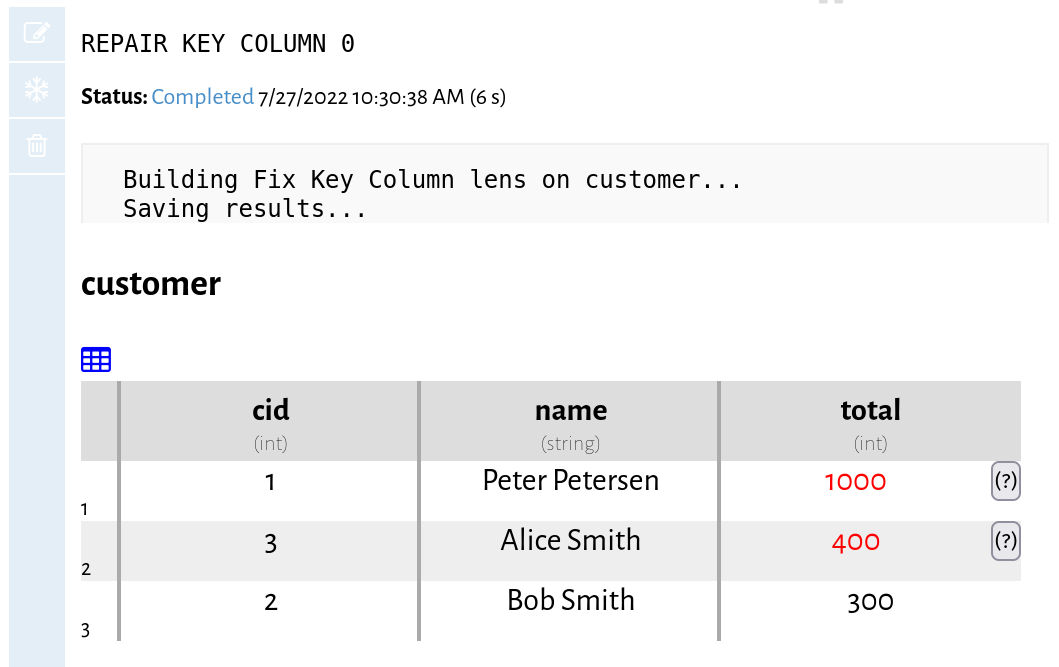
\includegraphics[width=8cm]{graphics/caveatted_data.png}
    % \begin{tabular}{c|c|c|c}
    %   \thead{cid} & \thead{name} & \thead{total} & \\       \hline
    %   1         & Peter          Petersen        & 1000 &   \\
    %   2         & Bob            Smith           & 300  & \rowcaveat  \\
    %   3         & Alice          Smith           & 400  & \rowcaveat  \\
    % \end{tabular}
    %%%%%%%%%%%%%%%%%%%%%%%%%%%%%%%%%%%%%%%%
  \caption{A UB-DB in Vizier encoding $D_1$ with possibly uncertain cells marked with caveats.}\label{fig:ub-db-encoding-d-2-with-p}
\end{wrapfigure}
%%%%%%%%%%%%%%%%%%%%%%%%%%%%%%%%%%%%%%%%
While such heuristics may be quite effective on average and are certainly superior to just randomly selecting a world, it is unavoidable that they fail for some cleaning scenarios. 
An alternative approach called consistent query answering~\cite{B11} takes a conservative stance, instead of selecting one repair, we reason about all possible repairs and only return query answers (the so-called \textit{certain answers}) that are in the query's results for every repair (i.e., are guaranteed to be in the result independent of which repair is correct). 
This approach has the advantage that only correct query answers are returned, but is computationally expensive, may exclude many very likely answers (if they are not 100\% certain), and is not closed (it is not possible to evaluate queries with certain answer semantics over the certain answers of a query).


%%%%%%%%%%%%%%%%%%%%%%%%%%%%%%%%%%%%%%%%%%%%%%%%%%%%%%%%%%%%%%%%%%%%%%%%%%%%%%%%
\subsection{Attribute- and Row-level Caveats and\\ Uncertainty-Annotated Databases}
\label{sec:attribute-row-level}
%
\begin{wrapfigure}[6]{r}[0pt]{8cm}
  \vspace*{-5mm}
  \centering
  \vspace*{-14mm}
  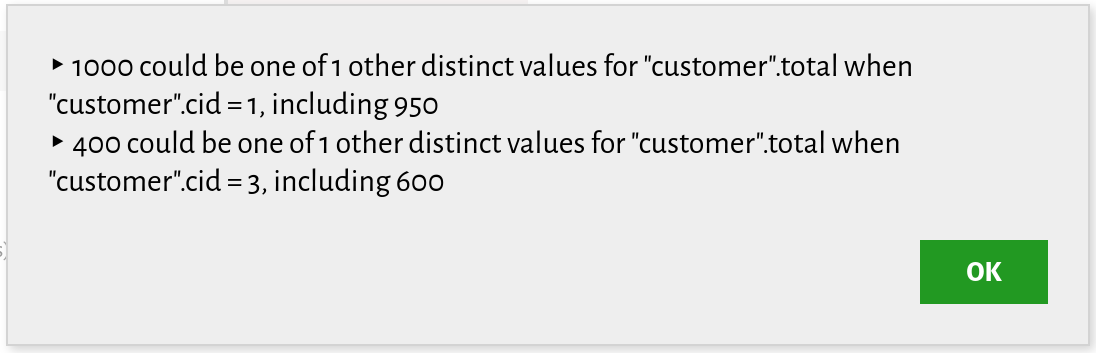
\includegraphics[width=8cm]{graphics/caveats.png}
  \caption{Caveats annotating the relation $D_1$}
\end{wrapfigure}
%


For Vizier, we developed an uncertain data model called
uncertainty-annotated databases~\cite{FH19} that annotates one
possible world (the so-called \textit{selected-guess world}) with an under-approximation  of certain answers (if we claim that a row is certain, then it is certain) that can be computed efficiently. This is encoded by annotating a subset of a dataset's rows with row-level caveats to mark them as not being certain.  The reason that we use an under-approximation is to be able to evaluate complex queries (full relational algebra including aggregation) efficiently (with PTIME data complexity and small overhead over deterministic query processing). Furthermore, attribute-level caveats are used to mark attribute values as uncertain (they may not be the same in every possible world) which is similar in nature to certain answers with nulls~\cite{L16a}.

% %%%%%%%%%%%%%%%%%%%%%%%%%%%%%%%%%%%%%%%%
% \begin{figure}[t]
%   \centering

% \begin{minipage}[b]{0.31\linewidth}
% \centering
%     \textbf{UA-DB with Selected Guess $D_1$}\\[3mm]
%     %%%%%%%%%%%%%%%%%%%%%%%%%%%%%%%%%%%%%%%
%     \begin{tabular}{c|c|c|c}
%       \thead{cid} & \thead{name} & \thead{total} & \\       \hline
%       1         & Peter          Petersen        & 1000 & \rowcaveat  \\
%       2         & Bob            Smith           & 300  & \rowcaveat  \\
%       3         & Alice          Smith           & 400  & \rowcaveat  \\
%     \end{tabular}
%     %%%%%%%%%%%%%%%%%%%%%%%%%%%%%%%%%%%%%%%%
%   \end{minipage}

%   \caption{UB-DB encoding $D_2$ with possibly uncertain rows marked with caveats (aster ix).}\label{fig:ub-db-encoding-d-2-with-p}
% \end{figure}
% %%%%%%%%%%%%%%%%%%%%%%%%%%%%%%%%%%%%%%%%

%%%%%%%%%%%%%%%%%%%%%%%%%%%%%%%%%%%%%%%%%%%%%%%%%%%%%%%%%%%%%%%%%%%%%%%%%%%%%%%%
% \subsection{Queries over Uncertainty-Annotated Databases}
% \label{sec:uncert-annot-datab}

% In~\cite{FH19} we introduced a query semantics for UA-DBs that

% %%%%%%%%%%%%%%%%%%%%%%%%%%%%%%%%%%%%%%%%%%%%%%%%%%%%%%%%%%%%%%%%%%%%%%%%%%%%%%%%
% \subsection{Implementation in Spark}
% \label{sec:implementation-spark}





%%% Local Variables:
%%% mode: latex
%%% TeX-master: "../2022_IEEE_DEB_Vizier"
%%% End:


%%%%%%%%%%%%%%%%%%%%%%%%%%%%%%%%%%%%%%%%%%%%%%%%%%%%%%%%%%%%%%%%%%%%%%%%%%%%%%%%
\section{Conclusions and Future Work}
\label{sec:conclusions}

In this paper, we have made the case for a multi-modal data science platform built on top of an incremental, data-centric workflow engine and have introduced the reader to Vizier, our system implementing this vision. 
Because each modality (notebooks, spreadsheets, the caveat view, etc\ldots) is a ``view'' interacting with the same underlying workflow and datasets, it is easy to extend the system to support new interaction paradigms in the future.  Building our system so that cells execute in isolation and only interact through dataflow makes it easy to add new cell types to the system, because we only have to worry about the interaction of the new cell type with  data artifacts. 
Thus, adding support for other interaction modalities (e.g., new programming languages) into the system is straight-forward: we implement a new cell type and an API to access Vizier artifacts from within the modality.

As demonstrated in recent preliminary work, having a scheduler that revises its schedule based on dependencies discovered at runtime and using static dataflow analysis, we can execute notebook cells in parallel and avoid re-executing cells that are guaranteed not to change during automatic refresh.
Significantly more opportunities for avoiding work exist, in particular by leveraging Vizier's standardized representation of artifacts.
For example, by representing updates to dataset artifacts as change sets, existing approaches for incremental view maintenance can reduce the runtime overhead of recomputing workflow steps, as well as the space costs of preserving multiple artifact versions. Another interesting direction for future work is to study incremental maintenance of workflow results when the definition of a workflow step changes. This is an novel variation of the traditional incremental view maintenance problem where we have to update the result based on a change to the query rather than based on a change to the data.

Similarly, standard representations of artifacts can be used to help users better understand the outputs of their workflows.
For example, numerous efforts have explored causal explanations in database query results (\cite{DBLP:conf/sigmod/KanagalLD11,DBLP:journals/pvldb/MeliouGMS11,DBLP:journals/pvldb/MeliouRS14,DBLP:journals/ftdb/GlavicMR21}, and explainability in machine learning has recently become an area of active research.
For such techniques to be truly valuable, they need to operate across artifact types. For example, what would it take to link a sudden change in predictions made by a model to the addition of a new category in source data five transformations removed from the model training step. With Vizier's uncertainty model and provenance tracking we lay the ground work to develop methods for generating explanations that span multiple steps in a workflow. 

Finally, we note that Vizier provides a ``ground-up'' approach to stitching different interaction modalities into a single workflow.
Tools implemented as views over Vizier's workflow model seamlessly interact with each other, with coarse-grained provenance, reactive cell execution, and repeatability/reproducibility.
However, these capabilities are limited to a single Vizier instance, and are of limited value to already existing tools.
An important open challenge is the design of a federated infrastructure for data analytics workflows, allowing multiple Vizier instances or unrelated tools to interoperate.


%%%%%%%%%%%%%%%%%%%%%%%%%%%%%%%%%%%%%%%%%%%%%%%%%%%%%%%%%%%%%%%%%%%%%%%%%%%%%%%%
% ACKNOWLEDGEMENTS
\mypara{Acknowledgements} This work was supported by NSF Awards ACI-1640864, IIS-1750460, IIS-1956149, and IIS-2125516. % and \ldots

%%%%%%%%%%%%%%%%%%%%%%%%%%%%%%%%%%%%%%%%%%%%%%%%%%%%%%%%%%%%%%%%%%%%%%%%%%%%%%%%
% BIBLIOGRAPHY
%\bibliographystyle{abbrv}
%\bibliography{2022_IEEE_DEB_Vizier.bib}

\documentclass[11pt]{article}

\usepackage{deauthor,times,graphicx}
\usepackage{color,colortbl}
% \usepackage[dvipsnames]{xcolor}
% \usepackage{hyperref}
\usepackage{amsmath}
\usepackage{amssymb}
\let\proof\relax
\let\endproof\relax
\usepackage{amsthm}
\usepackage{cleveref}
\usepackage{wrapfig}
\usepackage{url}
\usepackage{stmaryrd,amssymb}
\usepackage{listings}
\usepackage{algorithm}
% \usepackage[noend]{algorithmic}
\usepackage{fancybox}


%%%%%%%%%%%%%%%%%%%%%%%%%%%%%%%%%%%%%%%%
% Theorems, Definitions, Examples
%%%%%%%%%%%%%%%%%%%%%%%%%%%%%%%%%%%%%%%%
\newtheorem{theo}{Theorem}
\numberwithin{theo}{section}
\newtheorem{lem}[theo]{Lemma}
\newtheorem{propo}[theo]{Proposition}
\newtheorem{coll}[theo]{Corollary}
\newtheorem{exam}{Example}
\numberwithin{exam}{section}
\newtheorem{defi}{Definition}
\numberwithin{defi}{section}


%%%%%%%%%%%%%%%%%%%%%%%%%%%%%%%%%%%%%%%%%%%%%%%%%%%%%%%%%%%%%%%%%%%%%%%%%%%%%%%%
\usepackage{todonotes}
\newcommand{\BG}[1]{\todo[inline]{\textbf{Boris:} #1}}
\newcommand{\OK}[1]{\todo[inline]{\textbf{Oliver:} #1}}
\newcommand{\JF}[1]{\todo[inline]{\textbf{Juliana:} #1}}
\newcommand{\MB}[1]{\todo[inline]{\textbf{Mike:} #1}}

\newcommand{\jfedit}[1]{\textcolor{red} {#1}}


%%%%%%%%%%%%%%%%%%%%%%%%%%%%%%%%%%%%%%%%%%%%%%%%%%%%%%%%%%%%%%%%%%%%%%%%%%%%%%%%
% OUR SETUP
\newcommand{\mypara}[1]{\medskip\noindent\textbf{{#1}.}}

\ifdefined\thead
\else
  \newcommand{\thead}[1]{\textbf{#1}}
\fi
\newcommand{\rowcaveat}{\textbf{\textcolor{red}{$\ast$}}}
\newcommand{\pdb}{\mathcal{D}}

%%%%%%%%%%%%%%%%%%%%%%%%%%%%%%%%%%%%%%%%%%%%%%%%%%%%%%%%%%%%%%%%%%%%%%%%%%%%%%%%
% DOCUMENT
\begin{document}

%%%%%%%%%%%%%%%%%%%%%%%%%%%%%%%%%%%%%%%%%%%%%%%%%%%%%%%%%%%%%%%%%%%%%%%%%%%%%%%%
% LST DEFS

%%%%%%%%%%%%%%%%%%%%%%%%%%%%%%%%%%%%%%%%
% Colors
%%%%%%%%%%%%%%%%%%%%%%%%%%%%%%%%%%%%%%%%
\definecolor{lstpurple}{rgb}{0.5,0,0.5}
\definecolor{lstred}{rgb}{1,0,0}
\definecolor{lstreddark}{rgb}{0.7,0,0}
\definecolor{lstredl}{rgb}{0.64,0.08,0.08}
\definecolor{lstmildblue}{rgb}{0.66,0.72,0.78}
\definecolor{lstblue}{rgb}{0,0,1}
\definecolor{lstmildgreen}{rgb}{0.42,0.53,0.39}
\definecolor{lstgreen}{rgb}{0,0.5,0}
\definecolor{lstorangedark}{rgb}{0.6,0.3,0}
\definecolor{lstorange}{rgb}{0.75,0.52,0.005}
\definecolor{lstorangelight}{rgb}{0.89,0.81,0.67}
\definecolor{lstbeige}{rgb}{0.90,0.86,0.45}


% Declare bold typewriter font with Computer Modern
\DeclareFontShape{OT1}{cmtt}{bx}{n}{<5><6><7><8><9><10><10.95><12><14.4><17.28><20.74><24.88>cmttb10}{}

%%%%%%%%%% SQL + proveannce listing settings
\lstdefinestyle{psql}
{
tabsize=2,
basicstyle=\small\upshape\ttfamily,
language=SQL,
morekeywords={PROVENANCE,BASERELATION,INFLUENCE,COPY,ON,TRANSPROV,TRANSSQL,TRANSXML,CONTRIBUTION,COMPLETE,TRANSITIVE,NONTRANSITIVE,EXPLAIN,SQLTEXT,GRAPH,IS,ANNOT,THIS,XSLT,MAPPROV,cxpath,OF,TRANSACTION,SERIALIZABLE,COMMITTED,INSERT,INTO,WITH,SCN,UPDATED,PARTITION,BY,PRECEDING,FOLLOWING,CURRENT,ROW,ROWS,RANGE,GROUPING,SETS,CUBE,ROLL,UP},
extendedchars=false,
keywordstyle=\bfseries,
mathescape=true,
escapechar=@,
sensitive=true
}


%%%%%%%%%% SQL + proveannce listing settings - colorful version
\lstdefinestyle{psqlcolor}
{
tabsize=2,
basicstyle=\small\upshape\ttfamily,
language=SQL,
morekeywords={PROVENANCE,BASERELATION,INFLUENCE,COPY,ON,TRANSPROV,TRANSSQL,TRANSXML,CONTRIBUTION,COMPLETE,TRANSITIVE,NONTRANSITIVE,EXPLAIN,SQLTEXT,GRAPH,IS,ANNOT,THIS,XSLT,MAPPROV,OF,TRANSACTION,SERIALIZABLE,COMMITTED,INSERT,INTO,WITH,SCN,UPDATED},
extendedchars=false,
keywordstyle=\bfseries\color{lstpurple},
deletekeywords={count,min,max,avg,sum},
keywords=[2]{count,min,max,avg,sum,first,last,lead,lag,cxpath},
keywordstyle=[2]\color{lstblue},
stringstyle=\color{lstreddark},
commentstyle=\color{lstgreen},
mathescape=true,
escapechar=@,
sensitive=true
}


%%%%%%%%%% DATALOG style
\lstdefinestyle{datalog}
{
basicstyle=\footnotesize\upshape\ttfamily,
language=prolog
}




%%%%%%%%%% listings settings for pseudo code
\lstdefinestyle{pseudocode}
{
  tabsize=3,
  basicstyle=\small,
  language=c,
  morekeywords={if,else,foreach,case,return,in,or},
  extendedchars=true,
  mathescape=true,
  literate={:=}{{$\gets$}}1 {<=}{{$\leq$}}1 {!=}{{$\neq$}}1 {append}{{$\listconcat$}}1 {calP}{{$\cal P$}}{2},
  keywordstyle=\color{lstpurple},
  escapechar=&,
  numbers=left,
  numberstyle=\color{lstgreen}\small\bfseries,
  stepnumber=1,
  numbersep=5pt,
}

% \definecolor{pynotebookcellbg}{RGB}{247,247,247}
\definecolor{pynotebookcellbg}{gray}{0.95}

\lstdefinestyle{pynotebook}
{
  tabsize=3,
  basicstyle=\small\upshape\ttfamily,
  language=python,
  extendedchars=true,
  mathescape=true,
  morekeywords={show,read_csv,read_geojson,groupby,spatial_join,geocode,count},
  keywordstyle=\color{Blue},
  stringstyle=\itshape\color{Sepia},
  identifierstyle=\bfseries\color{OliveGreen},
  escapechar=&,
  numbers=left,
  numberstyle=\tiny\bfseries\ttfamily\color[gray]{0.7},
  stepnumber=1,
  numbersep=5pt,
  frame=single,
  frameround=tttt,
  backgroundcolor=\color{pynotebookcellbg}
}

\lstset{style=psqlcolor}

%%%%%%%%%%%%%%%%%%%%%%%%%%%%%%%%%%%%%%%%%%%%%%%%%%%%%%%%%%%%%%%%%%%%%%%%%%%%%%%%

\newcommand{\tinysection}[1]{
  \medskip \noindent \textbf{#1}.
}

%%%%%%%%%%%%%%%%%%%%%%%%%%%%%%%%%%%%%%%%%%%%%%%%%%%%%%%%%%%%%%%%%%%%%%%%%%%%%%%%
% TITLE AND AUTHORS
\title{The Right Tool for the Job: Data-Centric Workflows in Vizier}
%\title{It's a Notebook, It's a Spreadsheet, \ldots It's Vizier!}

\author{Oliver Kennedy,$^{\star}$~~Boris Glavic,$^{\diamond}$~~Juliana Freire,$^{\dagger}$~~and~~Michael Brachmann$\,^{\star}$\\
$^{\star}$~University at Buffalo, USA\\
$^{\diamond}$~Illinois Institute of Technology, USA\\
$^{\dagger}$~New York University, USA
}

\maketitle

\graphicspath{{submissions/workflow-vizier-glavic/}}

%%%%%%%%%%%%%%%%%%%%%%%%%%%%%%%%%%%%%%%%%%%%%%%%%%%%%%%%%%%%%%%%%%%%%%%%%%%%%%%%
% ABSTRACT
\begin{abstract}
  Data scientists use a wide variety of systems with a wide variety of
  user interfaces such as spreadsheets and notebooks for their data
  exploration, discovery, preprocessing, and analysis
  tasks. % For instance, spreadsheet interfaces are used for manual curation and simple types of analysis; notebook interfaces are used for data preprocessing, analysis, and visualization; and big data platforms, workflow systems, and database systems are used for more advanced querying and for deploying data analysis pipelines that were prototyped using notebooks.
  While this wide selection of tools offers data scientists the
  freedom to pick the right tool for each task, each of these tools
  has limitations (e.g., the lack of
  reproducibility % and automatic refresh of outdated results in
  of
  notebooks), % or the limited support of spreadsheets to specify batch data transformations),
  data needs to be translated between tool-specific formats, and
  common functionality such as versioning, provenance, and dealing
  with data errors often has to be implemented for each
  system. We argue that rather than alternating between task-specific
  tools, a superior approach is to build multiple user-interfaces on top
  of a single incremental workflow / dataflow platform with built-in
  support for versioning, provenance, error \& tracking, and data
  cleaning. We discuss Vizier, a notebook system that implements this
  approach, introduce the challenges that arose in building such a
  system, % , and compare the approach against state-of-the-art systems. Furthermore, we
  and highlight how our work on Vizier lead to novel research in
  uncertain data management and incremental execution of workflows.
\end{abstract}
%%%%%%%%%%%%%%%%%%%%%%%%%%%%%%%%%%%%%%%%%%%%%%%%%%%%%%%%%%%%%%%%%%%%%%%%%%%%%%%%


%%%%%%%%%%%%%%%%%%%%%%%%%%%%%%%%%%%%%%%%%%%%%%%%%%%%%%%%%%%%%%%%%%%%%%%%%%%%%%%%
\input{submissions/workflow-vizier-glavic/sections/introduction}
% \input{sections/requirements}
\input{submissions/workflow-vizier-glavic/sections/overview}
\input{submissions/workflow-vizier-glavic/sections/artifacts}
% \input{sections/microkernel_architecture}
\input{submissions/workflow-vizier-glavic/sections/vizier}
% \input{sections/microkernel_architecture}
\input{submissions/workflow-vizier-glavic/sections/symbolic_artifacts}
% \input{sections/notebook_view}
\input{submissions/workflow-vizier-glavic/sections/spreadsheets}
\input{submissions/workflow-vizier-glavic/sections/caveats}

%%%%%%%%%%%%%%%%%%%%%%%%%%%%%%%%%%%%%%%%%%%%%%%%%%%%%%%%%%%%%%%%%%%%%%%%%%%%%%%%
\section{Conclusions and Future Work}
\label{sec:conclusions}

In this paper, we have made the case for a multi-modal data science platform built on top of an incremental, data-centric workflow engine and have introduced the reader to Vizier, our system implementing this vision. 
Because each modality (notebooks, spreadsheets, the caveat view, etc\ldots) is a ``view'' interacting with the same underlying workflow and datasets, it is easy to extend the system to support new interaction paradigms in the future.  Building our system so that cells execute in isolation and only interact through dataflow makes it easy to add new cell types to the system, because we only have to worry about the interaction of the new cell type with  data artifacts. 
Thus, adding support for other interaction modalities (e.g., new programming languages) into the system is straight-forward: we implement a new cell type and an API to access Vizier artifacts from within the modality.

As demonstrated in recent preliminary work, having a scheduler that revises its schedule based on dependencies discovered at runtime and using static dataflow analysis, we can execute notebook cells in parallel and avoid re-executing cells that are guaranteed not to change during automatic refresh.
Significantly more opportunities for avoiding work exist, in particular by leveraging Vizier's standardized representation of artifacts.
For example, by representing updates to dataset artifacts as change sets, existing approaches for incremental view maintenance can reduce the runtime overhead of recomputing workflow steps, as well as the space costs of preserving multiple artifact versions. Another interesting direction for future work is to study incremental maintenance of workflow results when the definition of a workflow step changes. This is an novel variation of the traditional incremental view maintenance problem where we have to update the result based on a change to the query rather than based on a change to the data.

Similarly, standard representations of artifacts can be used to help users better understand the outputs of their workflows.
For example, numerous efforts have explored causal explanations in database query results (\cite{DBLP:conf/sigmod/KanagalLD11,DBLP:journals/pvldb/MeliouGMS11,DBLP:journals/pvldb/MeliouRS14,DBLP:journals/ftdb/GlavicMR21}, and explainability in machine learning has recently become an area of active research.
For such techniques to be truly valuable, they need to operate across artifact types. For example, what would it take to link a sudden change in predictions made by a model to the addition of a new category in source data five transformations removed from the model training step. With Vizier's uncertainty model and provenance tracking we lay the ground work to develop methods for generating explanations that span multiple steps in a workflow. 

Finally, we note that Vizier provides a ``ground-up'' approach to stitching different interaction modalities into a single workflow.
Tools implemented as views over Vizier's workflow model seamlessly interact with each other, with coarse-grained provenance, reactive cell execution, and repeatability/reproducibility.
However, these capabilities are limited to a single Vizier instance, and are of limited value to already existing tools.
An important open challenge is the design of a federated infrastructure for data analytics workflows, allowing multiple Vizier instances or unrelated tools to interoperate.


%%%%%%%%%%%%%%%%%%%%%%%%%%%%%%%%%%%%%%%%%%%%%%%%%%%%%%%%%%%%%%%%%%%%%%%%%%%%%%%%
% ACKNOWLEDGEMENTS
\mypara{Acknowledgements} This work was supported by NSF Awards ACI-1640864, IIS-1750460, IIS-1956149, and IIS-2125516. % and \ldots

%%%%%%%%%%%%%%%%%%%%%%%%%%%%%%%%%%%%%%%%%%%%%%%%%%%%%%%%%%%%%%%%%%%%%%%%%%%%%%%%
% BIBLIOGRAPHY
%\bibliographystyle{abbrv}
%\bibliography{2022_IEEE_DEB_Vizier.bib}

\input{submissions/workflow-vizier-glavic/2022_IEEE_DEB_Vizier.bbl}

\end{document}


\end{document}


\end{document}


\end{document}
